%%%%%%%%%%%%%%%%%%%%%% PRÉAMBULE


%%%%%%%%%%%%%% partie obligatoire du préambule
\documentclass[12pt,twoside]{book}
\usepackage{fontspec}
\usepackage{xunicode}
\usepackage{polyglossia}
\setmainlanguage{french}%indiquer la langue principale du document
\setotherlanguage{english} %indiquer les autres langues utilisée


%%%%%%%%%%%%%%%%%%%%%%%%%%%%%%%%% PACKAGES UTILISÉS

\usepackage{csquotes} % les guillemets français
\usepackage{lettrine} %faire une lettrine (pas obligatoire)

\usepackage[style=biblatex-enc/enc,sorting=nyt,maxbibnames=10]{biblatex}%charger le style de l'EnC (téléchargeable ici https://ctan.org/pkg/biblatex-enc)
\addbibresource{memoire-TNAH.bib} %le fichier bibliograhique.
%\defbibheading{}{\subsection*{}} Si l'on veut changer le titre de la/les bibliographie(s)


%%%Faire un ou plusieurs index

%\usepackage{imakeidx} %pour faire un ou plusieurs index
%\makeindex %commande pour générer l'index


%RAJOUTEZ ICI VOS PACKAGES

% Gestion des URL et des liens
\usepackage{url}            % Permet d'insérer et formater correctement les URL dans le texte

% Packages pour l'amélioration des tableaux
\usepackage{array}          % Offre plus d'options pour la création et la mise en forme des tableaux
\usepackage{booktabs}       % Crée des tableaux professionnels avec des lignes horizontales élégantes
\usepackage{tabularx}       % Génère des tableaux à largeur automatique avec colonnes flexibles
\usepackage{longtable}      % Gère les tableaux qui s'étendent sur plusieurs pages
\usepackage{ltxtable}       % Combine les fonctionnalités de longtable et tabularx

% Couleurs et code source
\usepackage{xcolor}         % Gestion avancée des couleurs (texte, tableaux, fond, etc.)
\usepackage{minted}         % Affichage de code source avec coloration avancée (utilise Pygments)

% Gestion des documents externes
\usepackage{pdfpages}       % Permet d'inclure des pages PDF externes directement dans le document

% Boucles et automatisation
\usepackage{pgffor}         % Fournit des commandes pour créer des boucles dans LaTeX (utile avec TikZ ou pour des tâches répétitives)

%%%%%%%%%%%%%%%%%%%%%%%%%%%%%%%%% CONFIGURATION DE MISE EN PAGE

%%%%%% Les compteurs (sections, subsections, etc)


%%%%%% Les compteurs (sections, subsections, etc)
\renewcommand{\thesection}{\Roman{section}.}%On ne fait apparaître que le numéro de la section
\renewcommand{\thesubsection}{\arabic{subsection}.}%subsection en chiffres arabes
\renewcommand{\thesubsubsection}{\alph{subsubsection}.}%subsubsection en lettres minuscules
%Si l'on veut faire apparaître les subsubsection dans le table des matières (à commenter sinon)
\setcounter{tocdepth}{3}
\setcounter{secnumdepth}{3}  % La subsubsection (profondeur=3 dans la table des matières) apparait numérotée dans la TdM



%%%%%  Configurer le document selon les normes de l'école

\usepackage[margin=2.5cm]{geometry} %marges
\usepackage{setspace} % espacement qui permet ensuite de définir un interligne
\onehalfspacing % interligne de 1.5
\setlength\parindent{1cm} % indentation des paragraphes à 1 cm


%%%%% Mise en forme des headers (haut de page)

\usepackage{fancyhdr} %package utilisé pour modifier les headers
\pagestyle{fancy} %utiliser ses propres choix de mise en page et non ceux par défaut du package

\setlength\headheight{16pt}%la hauteur des headers

%%la façon dont les sections apparaissent dans les en-tête:

\renewcommand{\sectionmark}[1]{\markright{\small\textit{\thesection~\  #1}}}%Faire apparaître dans les headers les sections en  petit et en italiques
%\renewcommand{\sectionmark}[1]{}%Commenter la lign précédetne et mettre celle-ci pour ne pas avoir le titre des sections dans le header

%% réglages propres à frontmatter

\appto\frontmatter{\pagestyle{fancy}%
	\renewcommand{\chaptermark}[1]{\markboth{\small\textit{#1}}{}}% ne pas faire apparaître de <<numéro>> de chapitre dans les chapitres non numérotés (front: l'introduction, els remerciement, etc)
}

%% réglages propres à mainmatter

\appto\mainmatter{
	\renewcommand{\chaptermark}[1]{\markboth{\small\chaptername~\thechapter~--\ \textit{#1}}{}}%faire apparaître dans les headers les sections en  petit et en italiques
}

%% réglages propres aux annexes

\appto\appendix{
	\renewcommand{\chaptermark}[1]{\markboth{\small~Annexe \thechapter~--\ \textit{#1}}{}}%faire apparaître dans les headers le nom des annexes
}


%indiquer des règles d'hyphénation pour des mots précis si besoin
%\begin{hyphenrules}{french}
%	\hyphenation{}
%\end{hyphenrules}


%%%%%%% Package hyperref

% A mettre après les autres appels de packages car redéfinit certaines commandes).

\usepackage[colorlinks=false, breaklinks=true, pdfusetitle, pdfsubject ={Mémoire HN}, pdfkeywords={les mots-clés}]{hyperref} %
\usepackage[numbered]{bookmark}%va avec hyperref; marche mieux pour les signets. l'option numbered: les signets dans le pdf sont numérotés

% Compléter pdfsubjet et pdfkeywords
%Explication des options de hyperref (modifiables)
% hyperindex=false
% colorlinks=false: pour que le cadre des liens n'apparaisse pas à l'impression
% breaklinks permet d'avoir des liens allant sur pusieurs lignes
%pdfusetitle: utiliser \author et \title pour produire le nom et le titre du pdf



%%%%%%%%%%%%%%%%%%%% Package glossaries

%Exception: il faut le charger APRÈS hyperref
\usepackage[toc=true]{glossaries}
\makeglossaries
%avec TexStudio: F9 pour compiler le glossaire (s'il y a aussi un index)

\loadglsentries{glossaire.tex}

%Structure d'une entrée de glossaire
%\newglossaryentry{}{%
	%	name={},%
	%	description={}
	%}



%%%%%%%%%%%%%%%%%% DÉFINITION DES COMMANDES ET ENVIRONNEMENTS %%%%%%%%%%%%%%%%%%

% ==== Bibliographie structurée par sections ====

% Définition d'un style de titre pour une sous-section de bibliographie
% - \refname est remplacé par le nom par défaut de la bibliographie
% - Titre imprimé sans numérotation
% - Ajout automatique de la sous-section dans la table des matières (toc)
\defbibheading{subbibintoc}[\refname]{%
  \subsection*{#1}% titre affiché, non numéroté
  \addcontentsline{toc}{subsection}{#1}} % ajout dans la table des matières

% Commande personnalisée pour afficher une partie de la bibliographie
% Paramètres :
%   #1 = mot-clé des références à afficher (défini dans le fichier .bib)
%   #2 = titre de la section de bibliographie
\newcommand{\myprintbiblio}[2]{%
  \printbibliography[heading=subbibintoc,keyword={#1},title={#2}]
}

% ==== Style pour le package minted ====

% Choix d'un style visuel prédéfini pour l'affichage du code
\usemintedstyle{tango}

% ==== Commande pour du code en ligne (inline) ====

% Commande générique pour insérer du code dans une ligne de texte
% Paramètres :
%   #1 = langage du code (ex: python, html, bash)
%   #2 = code à afficher
% Utilise minted avec options :
%   - breaklines : retour automatique à la ligne si le code est trop long
%   - breakanywhere : coupure possible à tout endroit
%   - breakautoindent : indentation automatique lors de la coupure
\newcommand{\codeinline}[2]{%
  \mintinline[breaklines, breakanywhere, breakautoindent=true]{#1}{#2}%
}

% ==== Environnement pour du code multi-ligne ====

% Création d'un environnement nommé "codeblock"
% Paramètre obligatoire : langage du code (ex: python, html)
\newenvironment{codeblock}[1]{%
  \VerbatimEnvironment
  \begin{minted}[
    fontsize=\small,
    breaklines,
    breakanywhere,			% gestion des coupures de lignes, n'importe où
    breakautoindent=true,	% Indentation pour les coupures de lignes
    linenos,                % Numérotation des lignes
    frame=single,           % Cadre simple autour du code
    framesep=3mm,           % Espacement entre code et cadre
    fillcolor=gray!5,       % Fond légèrement coloré
  ]{#1}}%
  {\end{minted}}

% ==== Commande pour afficher un fichier complet ====

% Permet d'inclure et afficher directement le contenu d'un fichier externe
% Paramètres :
%   #1 = langage du code (ex: python, html)
%   #2 = chemin du fichier à inclure
% Utilise les mêmes options visuelles que l'environnement codeblock
\newcommand{\codefile}[2]{%
  \inputminted[
    fontsize=\small,
    breaklines,
    breakanywhere,
    breakautoindent=true,
    linenos,
    frame=single,
    framesep=3mm,
    fillcolor=gray!5,
  ]{#1}{#2}%
}

%%%%%%%%%%%%%% INFORMATIONS POUR LA PAGE DE TITRE

\author{Amélie \textsc{Dogan} - M2 TNAH}
\title{Titre du mémoire}

%%%%%%%%%%%%%%%%%%%%%% DOCUMENT
\begin{document}
	\begin{titlepage}
		\begin{center}
			
			\bigskip
			
			\begin{large}				
				ÉCOLE NATIONALE DES CHARTES\\
				UNIVERSITÉ PARIS, SCIENCES \& LETTRES
			\end{large}
			\begin{center}\rule{2cm}{0.02cm}\end{center}
			
			\bigskip
			\bigskip
			\bigskip
			\begin{Large}
				\textbf{Amélie Dogan}\\
			\end{Large}
			%selon le cas
			\begin{normalsize} \textit{licenciée en histoire}
			\end{normalsize}
			
			\bigskip
			\bigskip
			\bigskip
			
			\begin{Huge}
				\textbf{Une \gls{edition-numerique} comme solution d'\gls{accessibilite} soutenable}\\
			\end{Huge}
			\bigskip
			\bigskip
			\begin{LARGE}
				\textbf{Étude autour de la base \textit{Philidor~4} du \gls{cmbv}}\\
			\end{LARGE}
			
			\bigskip
			\bigskip
			\bigskip
			\begin{large}
			\end{large}
			\vfill
			
			\begin{large}
				Mémoire 
				pour le diplôme de master \\
				\enquote{Technologies numériques appliquées à l'histoire} \\
				\bigskip
				2025
			\end{large}
			
		\end{center}
	\end{titlepage}
	
	\thispagestyle{empty}	
	\cleardoublepage
	
	\frontmatter
	
	\chapter{Résumé}
	
	\paragraph{En français} À l'ère numérique, les institutions patrimoniales font face à un défi majeur : comment rendre accessibles en ligne les corpus de données pour des publics diversifiés ? Ce mémoire explore cette tension à travers l'étude du \glslink{cmbv}{Centre de musique baroque de Versailles} et de sa base de données \textit{Philidor 4}. Ce travail examine l'évolution des outils numériques du \gls{cmbv} depuis trente ans et analyse les mutations qui ont accompagné le développement des bases de données patrimoniales. L'étude révèle comment la base de données \textit{Philidor 4} cristallise les enjeux contemporains de valorisation du patrimoine musical. Si son architecture répond aux exigences scientifiques, elle génère également des barrières ergonomiques qui limitent son appropriation. Face à ces constats, ce mémoire explore l'édition numérique statique comme solution complémentaire. À travers le développement d'un prototype \glslink{xml}{XML}/\glslink{xslt}{XSLT}, il démontre comment la transformation éditoriale des données peut produire des parcours thématiques plus accessibles et économiquement soutenables.
	
	\medskip
	
	\begin{english}
		\paragraph{In english} In the digital age, heritage institutions face a major challenge: how to make data collections accessible online to diverse audiences? This thesis explores this tension through a study of the \glslink{cmbv}{Centre de musique baroque de Versailles} and its \textit{Philidor 4} database. This work examines the evolution of the \gls{cmbv}'s digital tools over the past thirty years and analyzes the changes that have accompanied the development of heritage databases. The study reveals how the \textit{Philidor 4} database crystallizes the contemporary challenges of promoting musical heritage. While its architecture meets scientific requirements, it also creates ergonomic barriers that limit
		its appropriation. In light of these findings, this thesis explores static digital publishing as a complementary solution. Through the development of an \glslink{xml}{XML}/\glslink{xslt}{XSLT} prototype, it demonstrates how the editorial transformation of data can produce more accessible and economically sustainable thematic pathways.
	\end{english}
	
	\newpage
	
	\textbf{Mots-clés:} patrimoine musical, bases de données, accessibilité numérique, édition numérique statique, Centre de musique baroque de Versailles, Philidor, valorisation patrimoniale, médiation culturelle, musique baroque française, interopérabilité, ergonomie, architecture modulaire, XML, XSLT, institutions culturelles, numérisation patrimoniale, médiation numérique, éco-conception, sobriété numérique, transformation éditoriale, parcours thématiques, appropriation des données, musicologie numérique, humanités numériques.
	
	\textbf{Informations bibliographiques:} Amélie Dogan, \textit{Une \gls{edition-numerique} comme solution d'\gls{accessibilite} soutenable. Étude autour de la base \textit{Philidor~4} du \gls{cmbv}}, mémoire de master \enquote{Technologies numériques appliquées à l'histoire}, dir. Emmanuelle Bermès, École nationale des chartes, 2025.
	
	\newpage{\pagestyle{empty}\cleardoublepage}
	
	\chapter{Remerciements}
	
	\lettrine{C}e mémoire n'aurait pu voir le jour sans le concours et le soutien de nombreuses personnes que je souhaite remercier chaleureusement. Ma reconnaissance va d'abord à Mme Emmanuelle Bermès, ma directrice de mémoire, pour ses conseils éclairés, sa disponibilité et l'exigence scientifique qu'elle a su maintenir tout au long de ce travail. Ses relectures attentives et ses orientations méthodologiques ont été déterminantes dans l'aboutissement de cette recherche.
	
	Je tiens à exprimer ma profonde gratitude à l'équipe du \glslink{cmbv}{Centre de musique baroque de Versailles} qui m'a accueilli et accompagné avec une générosité remarquable. Mes remerciements s'adressent tout particulièrement à Julien Charbey, pour ses éclairages précieux sur l'histoire institutionnelle du \gls{cmbv}, à Laurent Guillo, pour m'avoir communiqué les archives des projets \textit{Philidor} et pour ses retours sur mon travail, et à Marco Lo Cascio, pour sa disponibilité et ses conseils. Leur confiance et leur ouverture ont rendu possible cette plongée dans l'univers complexe et passionnant des bases de données patrimoniales.
	
	Plus largement, je remercie l'ensemble du personnel du \gls{cmbv} pour leur accueil et leur contribution à ma compréhension des enjeux contemporains de la valorisation du patrimoine musical.
	
	Ma gratitude s'étend également à l'École nationale des chartes, à ses enseignants et à mes camarades de classe qui, par la richesse des échanges et des débats, a nourri ma réflexion et affiné ma méthode de travail.
	
	Je souhaite également remercier mes amis qui, par leurs encouragements constants et leur soutien moral, ont rendu ce parcours plus serein.
	
	Enfin, mes remerciements vont à ma famille, et notamment à ma maman dont les relectures bienveillantes et les questionnements ont contribué à clarifier ma pensée et à enrichir mon propos.
	
	Que tous ceux qui ont contribué, de près ou de loin, à l'accomplissement de ce travail trouvent ici l'expression de ma sincère reconnaissance.
	
	\newpage{\pagestyle{empty}\cleardoublepage}
	
	%%%%%%%%%%%% \bibliographie ici (normes de l'EnC)
	%%%%%%%%%%%% Bibliographie (normes de l'EnC)

\chapter{Bibliographie}

\section{Le \gls{cmbv} et la musicologie}
\myprintbiblio{CMBV}{Histoire du \gls{cmbv}}
\myprintbiblio{Source-primaire}{Archives des projets du \gls{cmbv}}
\myprintbiblio{Musicologie}{Musicologie et bibliothèque}

\section{Publication, édition et droit}
\myprintbiblio{Edition}{Questions d’éditorialisation}
\myprintbiblio{Droit}{Questions juridiques}

\section{Nouvelles technologies et patrimoine}
\myprintbiblio{Technologies}{Généralités sur les nouvelles technologies}
\myprintbiblio{Informatique-en-bibli}{Technologies appliquées au patrimoine}
\myprintbiblio{Low-Tech}{Technologies low-tech}
\myprintbiblio{Eco-conception}{Éco-conception}

\nocite{*} % Ajoute toutes les références non citées

	
	
	\chapter{Introduction}	
	
	\begin{quotation}
	\textit{\textquote{Ma messe est liturgique ... En mettant le Credo en musique, j'ai seulement voulu préserver le texte d'une manière particulière. On compose une marche pour aider les hommes à marcher ; ainsi, avec mon Credo, j'espère fournir une aide pour le texte.}}
\end{quotation}

C'est ainsi que s'exprimait Igor Stravinsky, un compositeur du XX\textsuperscript{e} siècle, au sujet d'une de ses messes. Cette réflexion du compositeur russe, bien qu'éloignée chronologiquement de la période baroque, cristallise une vérité fondamentale sur la fonction de la musique : celle-ci ne se contente pas d'exister en tant qu'art autonome, elle accompagne, soutient et révèle d'autres dimensions de l'expérience humaine. La musique devient ainsi un vecteur d'accès, une \textquote{aide} comme le formule Stravinsky, qui rend perceptible et accessible ce qui pourrait demeurer abstrait.

L'analogie que propose Stravinsky entre la composition musicale et la marche révèle une dimension pragmatique de l'art musical souvent occultée par les approches purement esthétiques. La mise en musique du texte sacré offre un support, un cadre qui guide la réception et la mémorisation. Cette fonction d'accompagnement, d'aide à la compréhension et à la transmission, traverse toute l'histoire de la musique occidentale. Elle se manifeste avec une acuité particulière dans la musique baroque française, où l'alliance du texte et de la mélodie, de la danse et du chant, de la cérémonie et de l'art, répond à des impératifs tant esthétiques que fonctionnels.

Cette conception fonctionnelle de la musique comme medium d'\gls{accessibilite} trouve un écho particulièrement pertinent dans les enjeux contemporains de la valorisation du patrimoine musical. À l'ère numérique, les institutions patrimoniales sont confrontées à un défi analogue : comment composer, non plus une marche ou un Credo, mais des outils numériques qui aident les chercheurs à chercher, les musiciens à interpréter, les enseignants à transmettre ? Comment préserver et transmettre l'immense corpus de la musique ancienne afin d'en faciliter l'accès et la compréhension ?

En effet, la révolution numérique a profondément transformé les modalités de conservation, d'étude et de diffusion du patrimoine musical. Les institutions culturelles disposent aujourd'hui de moyens techniques sans précédent pour numériser, cataloguer et mettre à disposition des corpus considérables. Cette démocratisation potentielle de l'accès aux sources musicales anciennes s'accompagne toutefois de nouveaux défis. L'accumulation exponentielle de données numériques pose des questions inédites en termes d'organisation, de structuration et surtout d'\gls{accessibilite} effective. La simple mise en ligne de documents numérisés ne suffit plus ; elle doit être accompagnée de dispositifs de \glslink{mediationculturelle}{médiation}, d'outils de recherche sophistiqués et d'interfaces adaptées aux différents publics. L'enjeu ne porte plus seulement sur la conservation des œuvres, mais sur leur capacité à demeurer vivantes, utilisables et signifiantes pour les communautés scientifiques, artistiques et éducatives contemporaines.

Cette problématique revêt une dimension particulièrement aigüe pour les musiques anciennes, dont la transmission repose sur des chaînes documentaires complexes. Entre les sources manuscrites originales, souvent lacunaires ou dispersées, les éditions critiques modernes et les interprétations contemporaines, se dessine un écosystème informationnel foisonnant mais fragmenté. Les bases de données patrimoniales tentent de cartographier ce territoire en reliant sources, œuvres, auteurs, interprètes et contextes historiques. Elles deviennent ainsi les nouveaux lieux de mémoire de la musique ancienne, mais leur efficacité dépend entièrement de leur capacité à être appropriées par leurs utilisateurs.

Le \gls{cmbv}, institution de référence pour la recherche, la diffusion et la valorisation du patrimoine musical français des XVII\textsuperscript{e} et XVIII\textsuperscript{e} siècles, s'inscrit pleinement dans cette logique d'accompagnement. Depuis sa création, il s'attache à construire des ponts entre la recherche académique, la pratique musicale vivante et la \gls{mediationculturelle}. Ses bases de données, fruit de décennies de travaux scientifiques, constituent un corpus exceptionnel recensant compositeurs, œuvres, sources, événements musicaux et interprètes de la période baroque française.

Toutefois, l'accumulation de ces données soulève aujourd'hui des questions cruciales d'\gls{accessibilite}. Comment garantir que ces ressources, issues de recherches approfondies, demeurent utilisables et pertinentes pour des publics aux besoins différenciés ? Comment concilier exhaustivité scientifique et facilité d'usage ? Comment les contraintes techniques et budgétaires contemporaines peuvent-elles orienter vers des solutions innovantes et durables ?

La base \textit{Philidor~4} du \gls{cmbv} cristallise ces enjeux. Conçue selon une architecture modulaire sophistiquée, elle offre un accès structuré à un corpus considérable tout en révélant certaines limites en termes d'ergonomie et de navigation. Face à ces défis, l'\gls{edition-numerique} statique émerge comme une solution complémentaire prometteuse, capable de transformer les données brutes en parcours éditorialisés, plus accessibles et contextualisés.

Ce mémoire se propose d'analyser cette tension entre accumulation patrimoniale et \gls{accessibilite} numérique, en étudiant comment une approche éditoriale peut constituer une réponse soutenable aux enjeux contemporains de valorisation du patrimoine musical numérique. La problématique centrale peut être formulée ainsi : dans quelle mesure l'\gls{edition-numerique} statique peut-elle offrir une solution complémentaire et soutenable aux limites d'\gls{accessibilite} des bases de données patrimoniales traditionnelles ?

Cette interrogation se décline selon plusieurs axes d'analyse. D'abord, il s'agira de comprendre les mutations qui traversent aujourd'hui les institutions patrimoniales face aux défis du numérique, en prenant l'exemple du \gls{cmbv} et de son évolution depuis trente ans. Puis, nous ferons un tour d'horizon des systèmes ayant été ou étant utilisés pour gérer, sauvegarder et diffuser les données du \gls{cmbv}. Ensuite, nous analyserons les potentiels et les limites de la base \textit{Philidor~4}, tant du point de vue technique qu'ergonomique, pour identifier les enjeux d'\gls{accessibilite} qu'elle soulève. Enfin, nous explorerons les possibilités offertes par l'\gls{edition-numerique} statique, en développant un prototype de site web thématique généré à partir des données de \textit{Philidor}.

La démarche adoptée articule analyse institutionnelle, étude technique et expérimentation pratique. Elle s'appuie sur une approche qualitative, combinant exploration des archives des projets numériques, analyse des outils existants et développement d'une solution prototype. Cette méthodologie permet d'ancrer la réflexion théorique dans une expérience concrète de manipulation des données et de création d'interfaces.

À travers l'exemple du \gls{cmbv} et de sa base \textit{Philidor~4}, nous explorerons ainsi les mutations institutionnelles, techniques et conceptuelles qui redéfinissent aujourd'hui les modalités d'accès aux corpus musicaux anciens, questionnant les formes contemporaines de cette \textquote{aide} que la technologie peut apporter à la transmission du patrimoine.
	
	\newpage{\pagestyle{empty}\cleardoublepage}
	
	%%%%%%%%%%%%%%%%%Le corps du mémoire
	\mainmatter
	%Trier par dossiers si besoin (front, main,annexes,), se crérer un docuemnt .tex par structure (section ou chapter selon la taille et la pertinence) Exemple de chemin à partir du dossier où se trouve le document maître: ./dossierA/fichier.tex
	
	
	
	\part[La patrimoine musical]{Le patrimoine musical numérique : enjeux institutionnels et défis techniques}
	
	La transformation numérique des institutions patrimoniales résulte d'un processus complexe, fait d'adaptations progressives, d'expérimentations techniques et de reconfigurations organisationnelles qui s'étalent sur plusieurs décennies. Pour comprendre les enjeux contemporains d'\gls{accessibilite} des bases de données patrimoniales, il convient d'abord de saisir les mutations profondes qui ont traversé ces institutions depuis l'avènement de l'informatique documentaire.
	
	Le \glslink{cmbv}{Centre de Musique Baroque de Versailles} offre un terrain d'observation privilégié de ces transformations. Institution hybride, à la fois centre de recherche, organisme de diffusion artistique et service de \gls{mediationculturelle}, le \gls{cmbv} a dû concilier des missions multiples tout en s'adaptant aux évolutions technologiques successives. Son parcours illustre les défis auxquels sont confrontées toutes les institutions patrimoniales : comment préserver et valoriser des corpus anciens avec les outils du présent ? Comment articuler exigences scientifiques, contraintes budgétaires et attentes des publics ?
	
	Cette première partie propose une analyse de ces mutations à travers deux prismes complémentaires. Le premier chapitre examine les enjeux institutionnels auxquels le \gls{cmbv} a dû faire face : redéfinition de ses missions à l'ère numérique, adaptation à de nouveaux publics, gestion des contraintes économiques et réglementaires. Le second chapitre retrace l'histoire technique des outils numériques utilisés par l'institution, depuis les premières bases de données jusqu'aux solutions contemporaines. Cette approche diachronique permet de comprendre comment les choix techniques d'hier conditionnent les possibilités d'aujourd'hui, et comment les institutions patrimoniales naviguent entre innovation et continuité, entre ambitions et contraintes.
	
	\chapter[Le \gls{cmbv}]{Le \gls{cmbv} : une institution face aux mutations numériques}

Créé en 1987 dans le contexte de redécouverte du patrimoine musical français, le \glslink{cmbv}{Centre de Musique Baroque de Versailles} a rapidement acquis une position de référence dans son domaine. Cependant, cette reconnaissance s'est construite dans un environnement en mutation constante : évolution des pratiques de recherche, diversification des publics, transformation des modes de diffusion culturelle. L'institution a dû sans cesse redéfinir son positionnement et ses méthodes pour demeurer pertinente.

Ce chapitre analyse la manière dont le \gls{cmbv} a négocié ces transformations. Il examine d'abord les missions fondamentales de l'institution et la typologie de ses publics, en montrant comment l'articulation entre recherche, pratique artistique et \glslink{mediationculturelle}{médiation} constitue à la fois la spécificité et la complexité du centre. Il étudie ensuite les défis contemporains de l'\gls{accessibilite} numérique, en montrant comment l'évolution des pratiques documentaires et les contraintes légales redessinent les contours de l'action patrimoniale. Il analyse enfin les stratégies développées par l'institution pour concilier ses ambitions scientifiques et culturelles avec les contraintes budgétaires qui pèsent sur le secteur patrimonial.

Cette approche institutionnelle permet de comprendre dans quel contexte organisationnel et stratégique s'inscrivent les développements techniques que nous analyserons par la suite. Elle révèle aussi les tensions structurelles qui traversent toute institution patrimoniale à l'ère numérique.

\section{Missions fondamentales et publics}

Pour comprendre les enjeux contemporains du \gls{cmbv}, il convient d'abord de retracer son histoire et de définir son positionnement institutionnel spécifique. Né de la rencontre entre une politique publique de valorisation patrimoniale et l'émergence du mouvement baroque, le centre s'est progressivement imposé comme un acteur incontournable de la scène musicale française. Cette section examine la genèse de l'institution, son statut juridique et ses missions officielles, avant d'analyser comment ces missions se traduisent concrètement dans l'articulation entre recherche académique, pratique musicale et \gls{mediationculturelle}. Elle s'attache enfin à caractériser les différents publics du centre --– chercheurs, musiciens, enseignants, grand public --– et leurs attentes souvent divergentes.

\subsection{Histoire et statut du \glslink{cmbv}{Centre de Musique Baroque de Versailles}}

\subsubsection{Genèse et contexte de création (1987-1989)}

Le \gls{cmbv} trouve ses origines dans un contexte particulièrement favorable à la redécouverte du patrimoine musical d'\gls{ancienregime}\footcite{buchernicolasSciencesPartageesPuisqu2022}. Les années 1980 sont marquées par l'essor du mouvement \textquote{Historiquement informé}. Ce mouvement prône le retour aux instruments d'époque et aux pratiques d'interprétation historiquement informées, s'opposant aux traditions romantiques du XIX\textsuperscript{e} siècle. En France, cette dynamique coïncide avec une prise de conscience politique de la richesse du patrimoine musical national, longtemps délaissé au profit du répertoire germanique.

Le \glslink{cmbv}{Centre de Musique Baroque de Versailles} a été officiellement créé en 1988 après une étude de faisabilité confiée par le Ministère de la Culture à Vincent Berthier de Lioncourt et Philippe Beaussant en 1987\footcite{CentreMusiqueBaroque}. Cette initiative s'inscrit dans une politique culturelle ambitieuse visant à \textquote{redonner au Château de Versailles sa musique et à la musique baroque française des XVII\textsuperscript{e} et XVIII\textsuperscript{e} siècles sa grandeur, sa justesse et son style originel}\footcite{CentreMusiqueBaroque}.

Cette mission fondatrice révèle une double ambition : patrimoniale, par la sauvegarde et la valorisation d'un répertoire oublié, et artistique, par la restitution des pratiques d'interprétation historiques. Le choix de Versailles n'est pas fortuit : symbole de la grandeur française sous l'Ancien Régime, le château incarne l'âge d'or de la musique de cour française, de Lully à Rameau.

\subsubsection{Évolution institutionnelle et développement des activités}

Les premières années du \gls{cmbv} sont marquées par une structuration progressive de ses activités autour de trois piliers fondamentaux : la recherche, la pratique musicale et la \glslink{mediationculturelle}{médiation}. Le tableau suivant reprend les grandes étapes et évolutions qui ont marqué l'histoire du \gls{cmbv}\footcite{CentreMusiqueBaroque} :

\begin{longtable}{p{2cm} p{13.5cm}}
	\caption{Évolution du \gls{cmbv} depuis sa création} \label{tab:evolution_cmbv} \\
	\toprule
	\textbf{Période} & \textbf{Étapes et évolutions} \\
	\midrule
	\endfirsthead
	
	\multicolumn{2}{c}%
	{{\bfseries \tablename\ \thetable{} -- suite de la page précédente}} \\
	\toprule
	\textbf{Période} & \textbf{Étapes et évolutions} \\
	\midrule
	\endhead
	
	\midrule \multicolumn{2}{r}{{Suite à la page suivante}} \\ \midrule
	\endfoot
	
	\bottomrule
	\endlastfoot
	
	1989 & Création de l'Atelier d'études sur la musique baroque française sous la direction de Jean Duron, axé sur la mise en partitions, la formation théorique des interprètes, le soutien scientifique et la diffusion des connaissances. Le projet pédagogique de la Maîtrise voit également le jour avec la mise en place du chœur d'hommes, Les Chantres. \\
	
	1990 & La Maîtrise s'enrichit d'un chœur d'enfants, les Pages. \\
	
	1991 & L'Atelier d'études est reconnu comme \textquote{jeune équipe du \gls{cnrs}} et prépare la mise en place de sa base de données \textit{Philidor}. \\
	
	1992 & Lancement des Éditions du \gls{cmbv} et création d'une bibliothèque spécialisée. L'Atelier d'études devient une \textquote{Unité de Recherche Associée au C.N.R.S.}. \\
	
	1993 & Le \gls{cmbv} s'ouvre à la scène internationale. \\
	
	1996 & Les différents départements du \gls{cmbv} s'installent à l'Hôtel des Menus-Plaisirs du Roy, leur emplacement actuel. \\
	
	1997 & Vincent Berthier de Lioncourt, son directeur et fondateur, quitte ses fonctions et est remplacé par Christian Oddos. \\
	
	1999 & Le \gls{cmbv} lance son premier site Internet. \\
	
	2000 & L'Atelier d'études est promu Unité Mixte de Recherche (UMR 2162) par le \gls{cnrs}. \\
	
	2008 & Le \gls{cmbv} s'engage dans le projet de recréer l'orchestre à cinq parties \textquote{à la française} des Vingt-quatre Violons du Roi. \\
	
	2017 & Les éditions du \gls{cmbv} achèvent la publication de l'intégrale des œuvres de Sébastien de Brossard, une première dans l'histoire de l'édition musicale française. \\
	
	2018 & Nicolas Bucher est nommé nouveau directeur général. \\
\end{longtable}

Cette chronologie révèle une \gls{institutionnalisation} progressive, marquée par la reconnaissance scientifique (rattachement au \gls{cnrs}), l'ancrage territorial (installation à l'Hôtel des Menus-Plaisirs) et l'ouverture internationale. L'évolution du statut de l'Atelier d'études, de \textquote{jeune équipe} à Unité Mixte de Recherche, témoigne de la maturité scientifique acquise par l'institution.

\subsubsection{Perspectives 2022-2024 et positionnement du \gls{cmbv}}

Sur la période 2022-2024, le \gls{cmbv} se donne pour objectif de s'affirmer comme un centre de ressources, de recherche, d'expérimentation, de création et de formation, en renforçant sa diffusion et en se connectant à la jeune génération\footcite{centredemusiquebaroquedeversaillesProjetEtablissement2022}. Cette ambition se traduit par des projets d'équipement ambitieux, notamment la volonté de créer un auditorium-studio d'enregistrement et des salles d'exposition et de projection à l'Hôtel des Menus-Plaisirs\footcite{centredemusiquebaroquedeversaillesProjetEtablissement2022}.

Le \gls{cmbv} se positionne désormais comme un \textquote{foyer de la musique française}, une maison pour les artistes, les chercheurs et le public, un lieu de convivialité et de combustion artistique\footcite{centredemusiquebaroquedeversaillesProjetEtablissement2022}. Cette vision témoigne d'une évolution vers un modèle plus ouvert et transversal, où la recherche académique dialogue étroitement avec la création contemporaine et la \gls{mediationculturelle}.

L'histoire du \gls{cmbv} est donc celle d'une institution qui a su constamment se réinventer face aux mutations de son environnement. L'évolution de ses statuts, le développement de ses différents pôles et l'établissement de ses locaux à l'Hôtel des Menus-Plaisirs du Roy sont autant de jalons qui ont consolidé sa place unique dans le paysage culturel français.

\subsection{Articulation entre recherche, pratique musicale et \glslink{mediationculturelle}{médiation}}

L'articulation entre la recherche académique, la pratique musicale et la \gls{mediationculturelle} est au cœur de la mission du \gls{cmbv}. Celle-ci s'est intensifiée avec le temps, notamment à travers une stratégie de transversalité.

\subsubsection{Recherche académique}

Le pôle Recherche s'efforce d'être dynamique et attractif. Ainsi, il a redéfini ses axes de recherche en 2022-2023 pour inclure la Fabrique, les Espaces, le Pouvoir et la Société, les Scènes et le Support à la Recherche\footcite{centredemusiquebaroquedeversaillesProjetEtablissement2022}\footcite{centredemusiquebaroquedeversaillesRapportActivite2023}. Il mène des projets d'envergure tels que Muséfrem\footnote{Musiciens d’Église en France à l’époque moderne}, AcadéC\footnote{Académies de Concert en France au XVIII\textsuperscript{e} siècle}, ThéPARis-France\footnote{théâtres en France sous l'Ancien Régime}, La cantate en France au XVIII\textsuperscript{e} siècle, et de nouveaux projets sur les Chansons d'oc et airs français dans les sources hébraïques et la musique des comédiens au XVII\textsuperscript{e} siècle. Un des grands enjeux de ces projets est d'identifier et d'étudier un patrimoine musical français mal connu et inédit, en dépassant l'opposition centre/provinces et en reconnaissant la spécificité des répertoires provinciaux\footcite{AcadeCAcademiesConcert}.

Le pôle accueille des chercheurs, dont des doctorants et des chercheurs externes au \glslink{cmbv}{Centre}, favorisant ainsi l'émergence de nouvelles recherches.\footcite{centredemusiquebaroquedeversaillesProjetEtablissement2022} De plus, le \gls{cmbv} est loin d'être une structure isolée, il est notamment rattaché au \gls{cnrs} via le Centre d'étude supérieur de la Renaissance (UMR7323, \gls{cnrs}/Université de Tours/Ministère de la Culture).\footcite{buchernicolasSciencesPartageesPuisqu2022}

\subsubsection{Pratique musicale et production artistique}

La Maîtrise du \gls{cmbv} est un pilier de la formation et de la production. Elle est composée des Pages et des Chantres. Les premiers sont des enfants de 7 à 14 ans\footcite{CentreMusiqueBaroquec}. Ils y reçoivent un enseignement vocal et choral. Les chantres sont quant à eux des adultes et bénéficient d'une formation très poussée en chant baroque. Les chantres et les pages participent ainsi à de nombreux concerts pédagogiques et à de nombreuses productions.

Le \gls{cmbv} soutient des recréations d'œuvres oubliées grâce aux recherches et aux éditions, en collaborant avec des ensembles et des artistes de renommée internationale\footcite{CentreMusiqueBaroque}. De plus, les éditions du \gls{cmbv} publient des partitions --- y compris des éditions monumentales et des partitions numériques augmentées via des partenariats comme Newzik --- et des ouvrages scientifiques, assurant la diffusion du patrimoine redécouvert par la recherche et rendu jouable\footcite{CentreMusiqueBaroque}. Les productions artistiques sont ainsi souvent liées à ces éditions\footcite{centredemusiquebaroquedeversaillesRapportActivite2023}.

L'équipe artistique est associée à l'étude et à la valorisation du répertoire, intégrant une visée pédagogique et collaborant avec des ensembles professionnels et des départements de musique ancienne des conservatoires.

\subsubsection{Médiation culturelle et action culturelle}

Le \gls{cmbv} vise une diffusion plus large de ses travaux et productions, en mettant l'utilisateur au centre de ses projets\footcite{centredemusiquebaroquedeversaillesProjetEtablissement2022}.

Le pôle Action culturelle, \glslink{mediationculturelle}{médiation} et publics se développe rapidement, visant à toucher des publics diversifiés. Des projets comme \textquote{Ville baroque}\footnote{à Maurepas et La Verrière} proposent des activités pluridisciplinaires incluant le chant, la danse, le théâtre et la musique électronique à des enfants et habitants, avec un objectif d'implantation pérenne\footcite{centredemusiquebaroquedeversaillesProjetEtablissement2022}.

Dans la même optique, on peut également citer les concerts participatifs à la Chapelle royale du château de Versailles qui sont organisés pour le public scolaire\footcite{centredemusiquebaroquedeversaillesRapportActivite2023}. De plus, le \gls{cmbv} structure son action vis-à-vis des enseignants de l'Éducation nationale en créant et diffusant des outils de ressources ainsi qu'en proposant des formations\footcite{centredemusiquebaroquedeversaillesProjetEtablissement2022}\footcite{centredemusiquebaroquedeversaillesRapportActivite2023}.

Des outils de \glslink{mediationculturelle}{médiation} innovants sont développés, notamment numériques, comme les \textquote{Expodcasts} et des playlists thématiques accessibles sur les plateformes de streaming\footcite{centredemusiquebaroquedeversaillesProjetEtablissement2022}.

Par ailleurs, le programme Lab'baroque soutient des ensembles émergents, intégrant concerts, \glslink{mediationculturelle}{médiation} et un accompagnement professionnel, tout en mesurant l'empreinte environnementale\footcite{centredemusiquebaroquedeversaillesRapportActivite2023}.

On note ainsi une synergie des pôles. La réussite du travail de transversalité se manifeste par des projets phares comme l'année de la Régence en 2023, qui a réuni tous les pôles du \gls{cmbv} (productions internationales, colloques de recherche, éditions de partitions et CD, expositions)\footcite{centredemusiquebaroquedeversaillesRapportActivite2023}. Le projet \textquote{Janus} avec l'\gls{ircam} en est un autre exemple, mêlant création contemporaine, formation, production artistique et action culturelle\footcite{centredemusiquebaroquedeversaillesRapportActivite2023}.

L'articulation réussie entre la recherche, la pratique et la \glslink{mediationculturelle}{médiation} constitue la véritable force du \gls{cmbv}. Le pôle Recherche identifie et étudie un patrimoine inédit, qui est ensuite rendu jouable grâce à la pratique musicale et aux éditions. Ce travail est finalement diffusé et rendu accessible au plus grand nombre par le pôle Médiation. Les projets phares, comme l'année de la Régence ou le projet \textquote{Janus} avec l'\gls{ircam}, illustrent parfaitement cette synergie qui permet à l'institution de rester pertinente et d'innover en permanence, en faisant dialoguer les siècles et les disciplines.

\subsection{Typologie des publics}

Le \gls{cmbv} s’adresse à une pluralité de publics, avec une attention particulière portée au renouvellement des générations. Cette diversité se reflète dans les profils accueillis, allant des chercheurs aux musiciens, en passant par les enseignants et le grand public\footcite{centredemusiquebaroquedeversaillesProjetEtablissement2022}.

\subsubsection{La communauté scientifique : chercheurs et partenaires institutionnels}

Le \glslink{cmbv}{Centre} collabore étroitement avec différents profils de chercheurs : permanents, associés ou ponctuellement accueillis, qu’ils soient affiliés au \gls{cmbv} ou à ses partenaires institutionnels tels que le \gls{cnrs}, le \gls{cesr}, l’\gls{iremus} ou la Fondation Royaumont\footcite{CentreMusiqueBaroque}. Ces chercheurs bénéficient d’un accès privilégié aux ressources documentaires et scientifiques du centre, notamment les bases de données spécialisées ainsi qu’aux fonds de la bibliothèque. Le \gls{cmbv} accorde également une place centrale aux jeunes chercheurs, spécifiquement les doctorants et post-doctorants, en leur offrant des opportunités d’accueil et d’accompagnement dans leur parcours professionnel et scientifique\footcite{centredemusiquebaroquedeversaillesProjetEtablissement2022}.

\subsubsection{Les musiciens : formation, accompagnement et collaboration artistique}

Comme nous l'avons évoqué en présentant brièvement la Maîtrise, le \gls{cmbv} s’investit fortement dans la formation et l’accompagnement des musiciens à différents stades de leur parcours. Il encadre ainsi les Pages. Ces derniers sont inscrits aux classes avec des horaires aménagés dans les cycles primaire et secondaire\footcite{CentreMusiqueBaroquec}. Il assure aussi la formation supérieure de chant baroque pour les Chantres et sanctionne leur parcours avec des examens exigeants. Le centre collabore étroitement avec plusieurs établissements d’enseignement supérieur comme les \gls{cnsmd} de Paris et de Lyon, le \gls{crr} de Versailles, le \gls{crr} de Paris, le \gls{crr} de Boulogne-Billancourt, le Pôle Supérieur de Paris – Boulogne-Billancourt, l'École supérieure des métiers du droit de Lille ou encore le Pôle Aliénor de Poitiers. Ces partenariats donnent naissance à des dispositifs variés : académies d’orchestre, masterclasses, stages d’immersion professionnelle ou encore programmes spécifiques comme \textit{Ballard} ou \textit{En Scène !}\footcite{centredemusiquebaroquedeversaillesProjetEtablissement2022}. Par ailleurs, de nombreux artistes professionnels --- solistes, chefs d’orchestre, ensembles, chorégraphes, danseurs, metteurs en scène --- participent aux productions et recréations artistiques du \gls{cmbv}, tout en ayant accès à ses ressources matérielles (partitions, instruments, locaux)\footcite{CentreMusiqueBaroque}. Enfin, le centre soutient la formation de jeunes chefs de chœur et de musiciens parmi lesquels on peut citer les \glspl{continuiste}\footcite{centredemusiquebaroquedeversaillesProjetEtablissement2022}.

\subsubsection{Le monde éducatif : enseignants et dispositifs pédagogiques}

Le \gls{cmbv} propose également des actions ciblées à destination des enseignants. Il accompagne les professeurs du premier et du second degré de l’Éducation nationale à travers des dispositifs de formation continue et la mise à disposition d’outils pédagogiques, notamment dans le cadre de projets comme \textquote{Ville baroque}\footcite{centredemusiquebaroquedeversaillesProjetEtablissement2022}. En parallèle, des professeurs de conservatoires et d’universités sont associés aux activités de recherche, en tant que membres des comités scientifiques ou intervenants dans les séminaires organisés par le centre\footcite{centredemusiquebaroquedeversaillesRapportActivite2023}.

Le jeune public, de l’école primaire au lycée, fait également l’objet d’actions de sensibilisation au patrimoine musical\footcite{centredemusiquebaroquedeversaillesProjetEtablissement2022}. On peut citer le programme \textquote{Bébé baroque} qui s'adresse aux plus petits\footcite{centredemusiquebaroquedeversaillesRapportActivite2023}.

\subsubsection{Le grand public : de la \glslink{mediationculturelle}{médiation} locale à la diffusion plus globale}

La programmation du \gls{cmbv} s’adresse aussi à un public élargi. Elle vise à toucher les mélomanes curieux de musique baroque ainsi que les visiteurs du Château de Versailles et de l’Hôtel des Menus-Plaisirs\footcite{centredemusiquebaroquedeversaillesProjetEtablissement2022}. Des actions culturelles et solidaires sont mises en œuvre à l’échelle locale, en lien avec les structures socio-culturelles, médico-sociales ou éducatives comme les centres sociaux, EHPAD, crèches, centres de loisirs et associations. Ces initiatives, portées par le pôle \gls{mediationculturelle}, prennent forme à travers des projets comme \textit{Générations Lully} ou encore \textit{Menus-Plaisirs d’été}. Par ailleurs, les \textit{Journées Découverte} et les \textit{Journées européennes du Patrimoine} ouvrent l'Hôtel des Menus-Plaisirs à un large public avec visites guidées, jeux de piste et ateliers\footcite{centredemusiquebaroquedeversaillesProjetEtablissement2022}. Enfin, le \gls{cmbv} étend sa portée à travers la diffusion de ses productions via des enregistrements discographiques, radiophoniques, audiovisuels (Mezzo, YouTube) et numériques (playlists)\footcite{centredemusiquebaroquedeversaillesRapportActivite2023}.

La pluralité des publics du \gls{cmbv} est le reflet de sa mission globale : être une institution inclusive et ouverte. En proposant des ressources et des actions ciblées pour les chercheurs, les musiciens en formation ou professionnels, les enseignants et le grand public, le centre s'assure que le patrimoine musical baroque ne reste pas réservé à une élite. Cette approche diversifiée, allant des partenariats universitaires aux programmes pour les tout-petits, positionne le \gls{cmbv} comme un acteur culturel et éducatif majeur.

En définitive, le \gls{cmbv} a su, depuis sa création, se structurer autour d'une synergie unique entre la recherche, la pratique musicale et la \glslink{mediationculturelle}{médiation}. Ses missions, qui se sont affinées avec le temps, le positionnent comme un acteur central dans la redécouverte et la diffusion du patrimoine musical baroque français. L'institution s'adresse à une pluralité de publics, des chercheurs aux mélomanes, en passant par les musiciens et les enseignants, ce qui témoigne de son approche et de son ambition à toucher le plus grand nombre. Cette assise solide est cependant mise à l'épreuve par les mutations contemporaines, en particulier celles liées au numérique, qui exigent de nouvelles stratégies d'adaptation pour pérenniser son modèle.

\section{Défis contemporains de l’\gls{accessibilite} numérique}

La transition numérique a profondément transformé les pratiques documentaires et les attentes des usagers des institutions culturelles. Cette section analyse les mutations qui traversent aujourd'hui le secteur patrimonial et leurs répercussions spécifiques sur l'activité du \gls{cmbv}. Elle examine d'abord l'évolution des pratiques de recherche, marquée par la généralisation des outils numériques et l'attente d'un accès immédiat à l'information. Elle explore ensuite la tension fondamentale entre exhaustivité scientifique et utilisabilité pratique, qui se manifeste particulièrement dans la conception des interfaces de recherche. Cette section aborde enfin les contraintes légales et éthiques qui encadrent désormais la mise en ligne des contenus patrimoniaux, du respect du droit d'auteur aux questions de propriété intellectuelle sur les données de recherche.

\subsection{Évolution des pratiques documentaires}

Le \gls{cmbv} est confronté aux mutations numériques comme toute institution. Ces mutations impactent profondément ses pratiques documentaires. La révolution numérique, caractérisée par la numérisation à grande échelle, l'interopérabilité des catalogues et les nouveaux modes d'accès, a redéfini la manière dont les collections musicales anciennes sont consultées, gérées et diffusées.

\subsubsection{Transformation des modes de consultation et de recherche}

La consultation et la recherche de sources musicales baroques ont connu une évolution majeure, passant d'un accès physique et restreint à une disponibilité numérique étendue. Avant l'ère numérique, la diffusion musicale reposait sur des éditions imprimées coûteuses et des manuscrits conservés dans des institutions spécifiques\footnote{\cite{dillonMusicManuscripts2011}}. Le répertoire français d'Ancien Régime est resté largement oublié après la Révolution jusqu'à son renouveau musicologique récent\footcite{CentreMusiqueBaroquea}.

L’essor des technologies a profondément transformé l’accès aux collections patrimoniales et musicales. Parmi les avancées les plus marquantes, on peut citer la mise en place de catalogues informatisés, la numérisation de masse, la production d’images en très haute résolution, l’exploitation du web de données ou encore le développement d’outils de reconnaissance automatique.

Ces innovations reposent sur des standards et protocoles communs qui assurent leur efficacité et leur interopérabilité. Par exemple, l’\gls{iiif} fournit un ensemble de spécifications techniques permettant de diffuser, d’échanger et de manipuler des images en haute résolution directement sur le web. Ce protocole permet par exemple la comparaison de plusieurs collections avec des options de zoom avancé qui permettent ainsi de casser les barrières géographiques\footcite{fresquetIIIFConnectivityMedieval}. Pour la modélisation et la description sémantique des données musicales, on s’appuie sur le \gls{rdf}, un modèle de données conçu pour représenter des ressources sur le web, ainsi que sur l’\gls{owl}, un langage basé sur \gls{rdf} qui permet de formaliser les connaissances sous la forme de concepts et de relations. Ces technologies s’inscrivent dans la dynamique plus large du \textit{\gls{web-semantique}}, dont l’objectif est de rendre les données non seulement accessibles, mais aussi compréhensibles et exploitables par des machines, favorisant ainsi la mise en relation automatique de contenus hétérogènes. Dans ce contexte, les interfaces de programmation d’application, en anglais \gls{api}, jouent un rôle central en offrant des interfaces normalisées pour interagir avec des services et des bases de données, facilitant la circulation et la réutilisation des informations entre différentes applications.

Dans le domaine de la reconnaissance automatique, des outils spécialisés ouvrent également de nouvelles perspectives. L’\gls{omr} permet de transformer une partition imprimée en un fichier informatique éditable et jouable, tandis que l’\gls{ocr} rend possible la transcription en texte numérique d’un document imprimé. Combinées avec des \gls{api} ouvertes, ces technologies peuvent être intégrées dans des chaînes de traitement plus complexes, par exemple en alimentant automatiquement des dépôts de données ou en enrichissant des environnements collaboratifs en ligne.

Ces différents développements, complémentaires les uns aux autres, constituent un socle technologique essentiel pour favoriser l’accès, l’enrichissement et la réutilisation des collections numériques.

Les implications pratiques de ces avancées sont notables. Elles permettent notamment des recherches et des analyses plus précises.

\subsubsection{Impact sur les métiers de la documentation musicale}

La mutation des pratiques documentaires a profondément transformé les métiers de la documentation musicale, exigeant l'acquisition de nouvelles compétences et l'émergence de nouveaux profils professionnels. Les compétences traditionnelles de catalogage sont désormais complétées par la modélisation \gls{rdf} et le web de données. L'indexation matière intègre l'utilisation d'\glspl{ontologie} et \glspl{taxonomie} musicales. La référence en salle s'est étendue à la \glslink{mediationculturelle}{médiation} en ligne. Enfin, la préservation physique des documents s'accompagne désormais de la préservation numérique et de la gestion de la pérennité des formats.

Cette évolution a donné naissance à de nouveaux profils à la croisée de l'informatique et des sciences humaines afin de répondre à ces nouvelles problématiques.

\subsubsection{Nouveaux usages}

D'autre part, plusieurs tendances d'usage émergent. À l'ère numérique, les usagers veulent avoir accès à tout et rapidement, de préférence sans bouger de chez soi ou n'importe où lorsque l'on est en déplacement. Les pratiques des chercheurs et des étudiants évoluent ; \textquote{pour eux, la recherche d’informations ne passe pas par les locaux de la bibliothèque, mais par un flux de documents et de données}\footcite{mesguichContexteEnjeux2017}. L'usager est conscient des mutations numériques et s'attend à ce que ces dernières lui facilitent ses recherches.

Parmi les innovations prisées, le \textquote{Search-to-score} permet l'intégration directe de la recherche à la partition numérique\footnote{Ex. : Newzik, nkoda} pour naviguer du catalogue à l'extrait sonore. Les annotations collaboratives offrent aux chercheurs et interprètes la possibilité de partager, en temps réel, variantes, doigtés ou traductions directement via l'interface \gls{iiif}. Par ailleurs, le \textquote{Mobile first} s'impose : 60~\% des consultations de partitions contemporaines se fait sur tablette, ce qui exige des formats réactifs et la possibilité d'annoter au stylet. Enfin, les plateformes de vidéo à la demande permettent à l'utilisateur d'écouter un enregistrement synchronisé avec la partition défilante.

Le \gls{cmbv} participe également à des initiatives comme le programme \gls{iccare}\footnote{Piloté par le \gls{cnrs}, le programme \gls{iccare} soutient la recherche pour accompagner les industries culturelles et créatives dans leur adaptation aux enjeux numériques, économiques et sociétaux.}. Ce dernier vise à fédérer les institutions culturelles autour de standards ouverts, et collabore avec des partenaires européens\footnote{Comme le \gls{cesr} Tours, le \gls{rism} Digital Center} pour le partage de \textit{\glspl{workflow}} de catalogage\footcite{ICCAREPartitionNumerique}. Le \gls{cmbv} contribue à cette dynamique en participant activement aux échanges et en accueillant dans ses murs les Journées d'accélération sur les partitions numériques du programme \gls{iccare}. Ces journées rassemblent des éditeurs, des bibliothécaires et des développeurs afin d'explorer les usages innovants de la partition numérique, en croisant les apports de l’intelligence artificielle, des technologies d’encodage et de reconnaissance musicale (\gls{ocr}/\gls{omr}) avec les besoins des chercheurs, musiciens et pédagogues\footcite{braudJourneesAccelerationICCARELAB2025}.

L'impact de la révolution numérique est manifeste sur les pratiques documentaires des institutions comme le \gls{cmbv}. La transition vers des formats et des protocoles standards comme \gls{iiif} et \gls{rdf}/\gls{owl} a ouvert la voie à une meilleure interopérabilité et à des recherches plus précises. Cette évolution nécessite toutefois le développement de nouvelles compétences, mêlant informatique et sciences humaines, pour gérer la numérisation, la préservation et la diffusion du patrimoine. En participant à des initiatives comme le programme \gls{iccare}, le \gls{cmbv} se positionne comme un acteur de la recherche dynamique, contribuant activement à l'avenir de la documentation musicale.

\subsection{Tensions entre exhaustivité et utilisabilité}

L'\gls{accessibilite} numérique du patrimoine musical baroque est constamment confrontée à une dialectique complexe entre l'impératif d'exhaustivité scientifique et l'exigence d'utilisabilité pour un public large. Effectivement, offrir une profondeur documentaire tout en garantissant une expérience utilisateur fluide et pertinente est un défi majeur pour les institutions patrimoniales.

\subsubsection{Attentes des différents utilisateurs}

L'ère numérique a redéfini les attentes des utilisateurs, qui recherchent un accès en ligne depuis chez eux au patrimoine musical. Le \gls{cmbv} s'adresse à une typologie de publics diversifiée, chacun ayant des attentes spécifiques. Les chercheurs universitaires exigent des métadonnées riches, des requêtes complexes et des exports dans différents formats de données ainsi que des identifiants \gls{rism}. Les interprètes professionnels recherchent des partitions prêtes à jouer fournies par les éditions du \gls{cmbv}. Les amateurs de musique baroque s'attendent quant à eux à du streaming et des playlists thématiques. Les enseignants demandent des ressources pédagogiques multimodales comme des conférences. Chaque public a donc ses propres attentes.

Les sources musicales baroques, par leur nature même, sont d'une richesse documentaire exceptionnelle, mais souvent complexe. Les manuscrits peuvent présenter des variantes, des corrections autographes, des indications de performance spécifiques à l'époque, et des systèmes de notation qui ne sont plus d'usage courant. Pour le chercheur ou le musicologue, cette exhaustivité est essentielle pour une compréhension approfondie de l'œuvre. Cependant, la transposition de cette richesse dans un environnement numérique peut rapidement nuire à la lisibilité pour l'utilisateur néophyte ou même pour l'interprète. Un fac-similé de manuscrit annoté avec toutes les divergences textuelles, si crucial pour un musicologue, peut être illisible pour un amateur cherchant simplement à écouter l'œuvre ou pour un musicien souhaitant une partition prête à jouer. Ainsi, aux éditions du \glslink{cmbv}{Centre}, beaucoup de questions entre en jeu au moment de lancer un projet.

Par ailleurs, une base de données présentant des œuvres musicales baroques pourra décrire plus ou moins finement l'œuvre en évoquant les pupitres, l'incipit textuel ou musical, les différents mouvements, le genre auquel appartient le texte, mais aussi celui auquel appartient la composition musicale. Toutes ces informations sont capitales pour les recherches, mais peuvent donner le vertige à un néophyte.

\subsubsection{Un exemple illustrant ces tensions : le projet Polifonia}

Cette tension se manifeste particulièrement dans les projets d'édition critique numérique. Si l'objectif est d'offrir l'intégralité des sources et des variantes, une interface trop chargée peut décourager l'utilisateur. Le projet Polifonia, financé par Horizon 2020, illustre cette problématique en cherchant à créer un espace numérique qui connecte les sources musicales à leur contexte historique tout en restant accessible au grand public\footcite{PolifoniaProjetRecherche2022}. L'enjeu majeur réside dans la capacité à proposer des interfaces différenciées selon les besoins et le niveau d'expertise des utilisateurs. Cela peut se traduire par des couches d'information superposables, des options de personnalisation de l'affichage, ou des parcours guidés\footcite{PolifoniaProjetRecherche2022}. L'objectif n'est pas de simplifier à l'excès, mais de rendre la complexité gérable et navigable. Les institutions doivent donc développer des compétences en design d'expérience utilisateur et en conception d'interfaces intuitives, tout en maintenant la rigueur scientifique dans la structuration des données sous-jacentes.

La conciliation de ces besoins parfois contradictoires est un exercice délicat. Le \glslink{cmbv}{Centre de Musique Baroque de Versailles} a développé des approches multi-niveaux intégrant formation, recherche et diffusion culturelle. Cela se traduit par la mise à disposition de bases de données sophistiquées pour les chercheurs, la publication d'éditions critiques pour les interprètes, et des actions de \glslink{mediationculturelle}{médiation} ou des outils numériques simplifiés pour le grand public et les pédagogues comme les conférences filmées. L'enjeu peut aussi être de créer des portes d'entrée multiples vers le même corpus de données, en adaptant le niveau de complexité et le mode de présentation sans jamais dénaturer l'information originelle.

Le défi de concilier exhaustivité et utilisabilité est au cœur de la stratégie numérique du \gls{cmbv}. L'institution reconnaît que les attentes des chercheurs ne sont pas celles du grand public ou des interprètes. La solution ne réside pas dans la simplification à outrance, mais dans la création de portes d'entrée multiples vers le même corpus de données. En développant des outils multi-niveaux et des interfaces intuitives, tout en préservant la rigueur scientifique de ses données sous-jacentes, le \gls{cmbv} montre qu'il est possible de rendre un patrimoine complexe navigable et pertinent pour tous, sans compromettre sa valeur scientifique.

\subsection{Contraintes légales et éthiques}

Le statut juridique du patrimoine musical baroque présente des spécificités complexes en matière de droits. Si les œuvres originales elles-mêmes relèvent du domaine public (généralement 70 ans après la mort de l'auteur, comme défini par le droit d'auteur\footcite{ChapitreIIIDuree}), leurs éditions modernes, les enregistrements et les arrangements contemporains demeurent protégés par des droits spécifiques en tant qu'œuvre seconde\footcite{barbryDroitsAuteurDroits1997}. Cette situation crée une superposition de régimes juridiques qui complique la diffusion numérique.

En effet, les œuvres originales sont dans le domaine public une fois le délai légal écoulé après la mort du compositeur. Cela permet, en théorie, leur libre exploitation. Par ailleurs, les éditions critiques contemporaines, même si elles portent sur des œuvres du domaine public, sont protégées par le droit d'auteur en tant qu'œuvres de l'esprit, en raison du travail éditorial\footcite{ChapitreIIOeuvres}. En effet, ce travail implique des recherches, des comparaisons entre les sources mais aussi des annotations qui y sont incorporés à l'œuvre originale. De plus, les enregistrements musicaux sont soumis aux droits voisins des interprètes et des producteurs, dont la durée de protection peut varier --- souvent 50 à 70 ans à partir de la fixation de l'enregistrement\footcite{martinoArtistesProducteursStreaming2019}. Enfin, les numérisations de documents physiques, qu'ils soient manuscrits ou imprimés, peuvent conférer des droits aux institutions patrimoniales qui ont réalisé la numérisation, protégeant ainsi l'investissement dans le processus\footcite{talbiInventionConceptPatrimoine2015}.

Cette complexité juridique oblige les institutions comme le \gls{cmbv} et la Bibliothèque nationale de France à des analyses minutieuses et souvent à des négociations complexes pour chaque projet de numérisation et de diffusion. La distinction entre une simple reproduction d'un document du domaine public et la création d'une nouvelle œuvre protégée, comme les éditions critiques et les enregistrements, est fondamentale et détermine les conditions d'accès.

À ces contraintes s’ajoute la question spécifique des travaux de recherche produits ou coordonnés par le \gls{cmbv}. Les projets menés par ses chercheurs, ou par des universitaires associés, aboutissent souvent à la constitution de bases de données spécialisées et de corpus numériques. Il peut s'agir de répertoires d’œuvres, d'inventaires de sources, de transcriptions encore d'éditions critiques. Ces ressources, bien qu’ayant pour objectif de favoriser la recherche et la diffusion du patrimoine, peuvent elles-mêmes être soumises à des restrictions liées aux droits d’auteur ou à la protection des bases de données\footcite{Directive96CE1996}. Ainsi, la réutilisation des données, même lorsque celles-ci décrivent des œuvres du domaine public, peut nécessiter une autorisation préalable si la structure, le contenu ou l’indexation résulte d’un travail original ou d’un investissement substantiel. Cette situation illustre la tension permanente entre les missions scientifiques et patrimoniales des institutions et les exigences juridiques qui encadrent la mise à disposition des ressources en ligne.

La gestion des droits est donc un enjeu de taille pour le \gls{cmbv}. La superposition des régimes juridiques, entre le domaine public des œuvres originales et les droits attachés aux créations dérivées, complique la diffusion numérique. Cette situation impose à l'institution d'opérer des analyses et des négociations complexes pour chaque projet. La protection des bases de données, qui peuvent être soumises à des restrictions malgré la nature publique du patrimoine qu'elles décrivent, ajoute une tension supplémentaire entre la mission scientifique de diffusion et les exigences légales. Le \gls{cmbv} doit donc naviguer avec prudence dans cet environnement juridique pour partager ses ressources tout en respectant ses obligations.

Les mutations numériques confrontent le \gls{cmbv} à des défis complexes. L'institution doit continuellement s'adapter à l'évolution des pratiques documentaires et aux nouveaux usages du public. La tension entre la rigueur scientifique, qui exige l'exhaustivité des données, et la nécessité de proposer des interfaces conviviales pour des publics variés demeure un enjeu central. Par ailleurs, le respect des contraintes légales et éthiques, notamment les droits d'auteur, complique la libre diffusion des ressources numériques. Le \gls{cmbv} relève ces défis en développant une expertise interne et en participant à des initiatives de recherche collaborative, tout en cherchant à démocratiser l'accès au patrimoine musical.

\section{Stratégies institutionnelles et contraintes budgétaires}

Les ambitions scientifiques et culturelles du \gls{cmbv} se heurtent aux réalités économiques contemporaines. Cette section examine de manière approfondie les contraintes budgétaires qui pèsent sur l'institution et leur impact sur les choix stratégiques, particulièrement en matière de développement numérique. Elle analyse d'abord l'évolution de la structure financière du centre depuis sa création et sa situation actuelle. Elle étudie ensuite les stratégies d'adaptation mises en œuvre par l'institution pour maintenir ses activités face à ces contraintes, privilégiant des approches pragmatiques et durables. Cette section présente enfin la stratégie numérique actuelle du \gls{cmbv}, qui articule maintien des outils existants, développement d'alternatives complémentaires et mutualisation avec d'autres institutions, tout en analysant les défis organisationnels liés aux ressources humaines spécialisées.

\subsection{Analyse des contraintes budgétaires}

Le \gls{cmbv} évolue dans un contexte économique particulièrement tendu, marqué par une fragilité budgétaire croissante qui sollicite fortement ses équipes et impacte directement le déploiement de ses activités. Cette situation s'inscrit dans une évolution historique des modèles de financement qui révèle les vulnérabilités structurelles de l'institution.

\subsubsection{Évolution des modèles de financement depuis la création}

Dès sa fondation, le \gls{cmbv} a expérimenté différents modèles de financement. Initialement soutenu par un partenariat public-privé, l'établissement a rapidement été confronté aux aléas du mécénat privé. La perte du soutien d'Alcatel Alsthom en 1996\footcite{CentreMusiqueBaroque} a marqué un tournant décisif, soulignant la vulnérabilité des financements dépendants d'acteurs uniques, particulièrement dans le secteur privé où les priorités stratégiques peuvent évoluer rapidement.

Cette expérience a conduit l'institution à repenser sa stratégie de financement. Le renforcement progressif de ses liens avec les institutions publiques s'est traduit par son association à l'Établissement Public du musée et du domaine national de Versailles\footcite{CentreMusiqueBaroque}, créant une première stabilisation institutionnelle. Plus récemment, le rattachement au \gls{cnrs}\footcite{CentreMusiqueBaroque} a constitué une étape majeure dans cette évolution. Ce rattachement présente un double avantage : d'une part, il consolide la légitimité scientifique de l'établissement en l'inscrivant pleinement dans l'écosystème de la recherche publique française ; d'autre part, il ouvre de nouvelles voies de financement spécifiquement dédiées à la recherche académique, notamment par l'accès aux programmes \glslink{anr}{ANR} et aux financements européens\footnote{Cette évolution s'inscrit dans la tendance générale de professionnalisation de la recherche en sciences humaines et sociales, où l'adossement institutionnel devient crucial pour l'accès aux financements compétitifs.}.

Malgré cette diversification progressive, le modèle économique du \gls{cmbv} reste complexe, articulant subventions ministérielles, soutiens des collectivités locales, financements de projets et ressources propres. Cette multiplicité des sources, si elle offre une certaine résilience, génère également une complexité administrative considérable et une incertitude récurrente sur les ressources disponibles à moyen terme.

\subsubsection{Situation financière actuelle et difficultés structurelles}

L'exercice 2023 illustre de manière particulièrement saisissante les tensions financières auxquelles fait face le \gls{cmbv}. Malgré des efforts conséquents déployés par la direction pour réduire les charges de fonctionnement, l'année a débuté avec un déficit prévisionnel de 250~000 euros\footcite{centredemusiquebaroquedeversaillesRapportActivite2023}. Cette situation critique s'inscrit dans un contexte plus large de fragilisation des équilibres financiers de l'établissement.

La perte de certains soutiens structurels a aggravé cette situation déjà tendue. L'arrêt de l'accord d'avances de trésorerie avec la Société Générale\footcite{centredemusiquebaroquedeversaillesRapportActivite2023} a notamment privé l'institution d'un instrument financier essentiel. Pour préserver son équilibre, le \gls{cmbv} a dû bénéficier de l'intervention exceptionnelle du Ministère de la Culture. Celui-ci a versé deux aides ponctuelles de 200~000 euros chacune\footcite{centredemusiquebaroquedeversaillesRapportActivite2023}, permettant de maintenir l'équilibre financier immédiat. Ces interventions, bien que salutaires, soulignent la précarité financière de l'établissement.

Les charges de fonctionnement connaissent par ailleurs une augmentation constante. Les dépenses liées aux ressources humaines, qui constituent le poste le plus important du budget, subissent les effets de l'inflation salariale. La maintenance des outils numériques représente un poste en croissance permanente, nécessitant des mises à jour régulières, des migrations technologiques coûteuses et le recours à des prestataires spécialisés. Par ailleurs, l'entretien des instruments historiques et des locaux patrimoniaux de l'Hôtel des Menus-Plaisirs génère également des coûts significatifs et imprévisibles\footcite{centredemusiquebaroquedeversaillesProjetEtablissement2022}.

\subsubsection{Impact sur les missions prioritaires et les investissements numériques}

Ces contraintes financières se répercutent directement sur les capacités d'action de l'établissement. Le poste communication illustre bien cette problématique : représentant moins de 3~\% du budget total du \gls{cmbv}\footcite{centredemusiquebaroquedeversaillesProjetEtablissement2022}, un montant jugé insuffisant pour assurer une visibilité à la hauteur de la qualité et de la diversité des travaux menés par le centre. Cela restreint mécaniquement la diffusion des productions scientifiques, pédagogiques et artistiques du \gls{cmbv}, limitant ainsi son rayonnement et, par effet de retour, ses capacités à attirer de nouveaux partenaires.

L'exposition à la précarité des financements par projet constitue un autre facteur de vulnérabilité. L'exemple du programme \textit{En Scène !}, qui n'a pu être reconduit en raison de l'absence de renouvellement des crédits spécifiques qui le soutenaient\footcite{centredemusiquebaroquedeversaillesRapportActivite2023}, illustre parfaitement cette problématique. Ce cas révèle les limites d'un modèle économique reposant sur des financements ponctuels, où la continuité des actions dépend de décisions externes souvent déconnectées des besoins de l'institution.

Dans le domaine numérique spécifiquement, la maintenance continue des systèmes d'information représente un investissement conséquent, tant en ressources financières qu'humaines. Les migrations technologiques et les développements spécialisés nécessitent fréquemment le recours à des prestataires externes comme Acatus, créant une dépendance technique et financière préoccupante. Cette situation engendre plusieurs risques majeurs : la discontinuité de service en cas de changement de prestataire, l'augmentation progressive des coûts de maintenance spécialisée, et une perte potentielle de contrôle sur l'évolution technique des systèmes.

Les investissements d'envergure, comme le projet de construction d'un auditorium-studio d'enregistrement associé à des espaces d'exposition et de projection, illustrent parfaitement les tensions entre ambition et réalité économique. Ce chantier, essentiel pour le rayonnement futur de l'institution, implique un plan de financement complexe mobilisant plusieurs sources\footnote{Conseil régional, Ministère de la Culture, mécénat}, dont l'aboutissement conditionne la réalisation effective du projet\footcite{centredemusiquebaroquedeversaillesProjetEtablissement2022}. L'incertitude sur la concrétisation de ces financements croisés illustre la complexité croissante des montages financiers nécessaires pour mener à bien des projets structurants.

\subsection{Stratégies d'adaptation institutionnelle}

Face à ces contraintes budgétaires majeures, le \gls{cmbv} a développé un ensemble cohérent de stratégies d'adaptation qui témoignent de sa capacité de résilience. Ces stratégies s'articulent autour de trois axes principaux : l'optimisation de l'organisation interne, la diversification des ressources et la valorisation des moyens existants.

\subsubsection{Renforcement de la transversalité interne}

L'année 2023 a été marquée par un effort structurel significatif de réorganisation interne, visant à optimiser l'efficacité opérationnelle malgré la contrainte des effectifs. Dans l'édito du rapport d'activités 2023, la direction du \gls{cmbv} souligne avec satisfaction que, malgré les difficultés financières persistantes, l'établissement est parvenu à maintenir une programmation dynamique et exigeante\footcite{centredemusiquebaroquedeversaillesRapportActivite2023}.

Cette performance s'explique en grande partie par un travail approfondi de réorganisation qui a permis de décloisonner les services et d'encourager une meilleure articulation entre les différents pôles de l'institution : Recherche, Éditions, Formation, Production et Action Culturelle\footcite{centredemusiquebaroquedeversaillesRapportActivite2023}. Cette logique de décloisonnement s'appuie sur la reconnaissance que les compétences développées dans chaque pôle peuvent être mutualisées et enrichies par les apports des autres secteurs.

La mise en œuvre concrète de cette transversalité s'est illustrée de manière exemplaire dans le programme consacré à la Régence. Ce projet ambitieux a mobilisé l'ensemble des compétences du centre, créant des synergies inédites entre les équipes et démontrant la richesse potentielle de cette approche collaborative\footcite{centredemusiquebaroquedeversaillesRapportActivite2023}. Les chercheurs ont ainsi pu bénéficier directement de l'expertise éditoriale pour optimiser la valorisation de leurs travaux, tandis que les équipes de formation ont intégré les dernières découvertes scientifiques dans leurs programmes pédagogiques.

Cette stratégie organisationnelle présente plusieurs avantages stratégiques. Elle permet d'abord de compenser partiellement la réduction des effectifs en optimisant l'utilisation des compétences disponibles. Elle favorise ensuite l'innovation par le croisement des expertises et la circulation des idées entre les différents métiers. Elle contribue enfin à renforcer la cohérence globale des actions du centre, évitant les redondances et maximisant l'impact des réalisations.

\subsubsection{Diversification des sources de revenus}

Dans une perspective d'autonomisation financière progressive, le \gls{cmbv} développe activement une stratégie de diversification de ses ressources qui vise à réduire sa dépendance aux subventions publiques traditionnelles.

Le développement du mécénat constitue l'un des axes prioritaires de cette diversification. L'institution multiplie donc les démarches auprès d'entreprises. Parallèlement, elle développe une approche plus systématique du mécénat de particuliers, notamment via le Cercle Rameau\footcite{centredemusiquebaroquedeversaillesProjetEtablissement2022}. Cette structure permet de fidéliser un réseau d'amateurs éclairés et de donateurs réguliers, créant une base de financement plus stable et prévisible.

La recherche de partenariats avec des fondations représente un autre levier stratégique majeur. Ces institutions, spécialisées dans le soutien à la culture et à la recherche, peuvent financer des projets spécifiques ou soutenir des dispositifs de bourses, en complément des subventions publiques traditionnelles\footcite{centredemusiquebaroquedeversaillesProjetEtablissement2022}. Cette approche nécessite une professionnalisation accrue des démarches de recherche de financement et une capacité renforcée à présenter les projets dans les formats attendus par ces partenaires potentiels.

L'inscription dans des réseaux européens et internationaux ouvre également de nouvelles perspectives de financement. Ces financements, bien que complexes à obtenir, peuvent représenter des montants significatifs et contribuer simultanément au rayonnement international de l'institution.

\subsubsection{Optimisation des ressources existantes}

L'optimisation des ressources constitue le troisième pilier de la stratégie d'adaptation du \gls{cmbv}. Cette approche vise à maximiser la valeur et l'usage des investissements déjà réalisés, tant en termes d'infrastructure que d'équipements ou de collections.

La valorisation des espaces, en particulier l'Hôtel des Menus-Plaisirs, représente un enjeu majeur dans cette logique d'optimisation. Ce lieu chargé d'histoire offre un potentiel considérable pour l'accueil d'événements, la location d'espaces ou le développement d'activités génératrices de revenus complémentaires\footcite{centredemusiquebaroquedeversaillesProjetEtablissement2022}. L'objectif est de transformer ce patrimoine architectural en véritable atout économique, sans compromettre sa fonction première de lieu de travail et de création.

L'enrichissement continu du parc instrumental constitue un autre aspect de cette stratégie d'optimisation. Chaque acquisition d'instrument historique ou de copie d'époque renforce simultanément les capacités pédagogiques, de recherche et de production artistique de l'institution\footcite{centredemusiquebaroquedeversaillesProjetEtablissement2022}. Cette approche intégrée permet de maximiser l'impact de chaque investissement en le faisant servir à plusieurs missions simultanément.

Dans le domaine numérique, l'optimisation passe par une rationalisation des outils et des processus. L'objectif est de tirer le maximum de valeur des systèmes existants avant d'envisager de nouvelles acquisitions, tout en préparant les évolutions technologiques nécessaires. Cette approche équilibrée permet de concilier continuité opérationnelle et innovation technologique dans un contexte de ressources contraintes.

\subsection{Stratégie numérique et défis techniques}

Le \gls{cmbv} développe depuis plus de trente ans une stratégie numérique ambitieuse, centrée sur la création, la gestion et la diffusion de ressources numériques scientifiques dédiées à la musique française des XVII\textsuperscript{e} et XVIII\textsuperscript{e} siècles\footcite{RessourcesNumeriquesCentre}. Cette stratégie, confrontée aux défis contemporains de l'\gls{accessibilite} numérique dans un contexte de contraintes financières, nécessite des adaptations constantes et une vision prospective pour assurer la pérennité des investissements numériques.

\subsubsection{Orientations stratégiques : migration et interopérabilité}

Face aux enjeux de pérennité technologique, le \gls{cmbv} a développé plusieurs orientations stratégiques majeures qui guident ses choix techniques et organisationnels. La première de ces orientations concerne la migration progressive vers des solutions recommandées et validées par la communauté scientifique et universitaire. Cette approche s'appuie sur la reconnaissance que la durabilité des outils numériques dépend largement de leur adoption par des communautés larges et actives, garantissant leur maintenance et leur évolution à long terme.

L'un des défis les plus critiques demeure la migration permanente des anciens systèmes vers des plateformes plus modernes et pérennes. Cette exigence impose aux équipes du \gls{cmbv} de maintenir une veille technologique permanente, particulièrement complexe dans un environnement où les innovations se succèdent rapidement. Cette veille vise à anticiper l'obsolescence des technologies actuellement utilisées, identifier les solutions de remplacement les plus appropriées et adapter les méthodologies de travail en conséquence\footnote{Cet aspect sera développé en profondeur lors de la présentation détaillée des outils du \gls{cmbv} dans le chapitre suivant.}.

L'utilisation systématique de formats standards constitue un autre pilier de cette stratégie. Ces formats, garantissant l'interopérabilité future des systèmes, permettent d'éviter les situations de dépendance technologique qui peuvent compromettre l'accès aux données à long terme. Le défi de l'interopérabilité revêt une dimension particulièrement critique pour garantir la compatibilité future des systèmes d'information du centre avec les plateformes externes. Dans cette optique, le \gls{cmbv} s'attache à adopter des standards ouverts et des protocoles normalisés reconnus internationalement. Cette approche facilite notamment le moissonnage et l'échange de données avec les plateformes nationales et européennes de référence, telles que Gallica et Europeana. L'utilisation des identifiants \gls{rism} s'inscrit pleinement dans cette logique d'interopérabilité, permettant une identification univoque et pérenne des ressources musicales.

L'objectif ultime de ces choix techniques est de garantir la lisibilité des formats sur le long terme, évitant ainsi la perte d'\gls{accessibilite} aux données numériques du centre. L'adoption de formats ouverts et normalisés présente l'avantage majeur que leurs spécifications sont publiquement disponibles et documentées\footnote{Cette exigence s'inscrit dans le cadre réglementaire français, notamment la Loi n°~2004-575 du 21 juin 2004 pour la confiance dans l'économie numérique, article 4.}, ce qui permet, en cas d'obsolescence d'un système, de maintenir ou de recréer les outils nécessaires à la lecture des documents.

L'architecture technique privilégiée par le \gls{cmbv} s'oriente vers des solutions modulaires et évolutives, permettant des adaptations progressives sans remise en cause complète des systèmes existants. Cette approche présente l'avantage de répartir les coûts de migration dans le temps et de minimiser les risques de rupture de service.

\subsubsection{Documentation technique et enjeux de traçabilité}

Le maintien d'une documentation technique exhaustive et actualisée constitue un enjeu majeur pour la pérennité des systèmes d'information du \gls{cmbv}. Cette documentation, indispensable à la compréhension, à l'évolution et à la maintenance des systèmes numériques, représente néanmoins un investissement considérable en temps et en ressources humaines spécialisées.

À ce jour, la documentation des outils en place demeure partiellement lacunaire, situation qui peut considérablement compliquer la compréhension de l'existant. Ces lacunes se révèlent particulièrement problématiques lors des phases critiques de maintenance corrective, de migration technologique ou de montée en compétence de nouveaux intervenants. L'absence de documentation détaillée peut transformer des opérations techniques de routine en projets complexes et coûteux.

Face à ce constat, le \gls{cmbv} s'efforce d'améliorer systématiquement plusieurs aspects cruciaux de sa documentation technique. La création et la mise à jour régulière des guides d'utilisation associés aux outils constituent une priorité immédiate. Ces documents doivent être suffisamment détaillés pour permettre une prise en main autonome tout en restant accessibles aux non-spécialistes.

La documentation détaillée des processus de migration et d'archivage revêt une importance stratégique particulière. Ces procédures, indispensables pour garantir la réversibilité et la cohérence des évolutions techniques, doivent être suffisamment précises pour permettre leur reproduction par d'autres équipes ou prestataires. Cette exigence est d'autant plus critique que les migrations technologiques sont souvent réalisées sous contrainte temporelle et budgétaire.

Cette documentation technique représente bien plus qu'un simple support à l'exploitation courante : elle constitue un véritable levier stratégique pour accompagner les transitions technologiques à venir. Une documentation de qualité peut considérablement réduire les coûts et les risques associés aux évolutions futures, tout en facilitant la transmission des savoir-faire techniques au sein de l'équipe.

\subsubsection{Impact du départ de Laurent Guillo et adaptations organisationnelles}

Le départ à la retraite de Laurent Guillo, responsable des données numériques au \gls{cmbv} de 2019 à 2024\footcite{GuilloLaurentCESR}, au début de l'année 2025, constitue un défi organisationnel majeur pour l'institution. L'absence de remplacement immédiat soulève des questions fondamentales sur la continuité de la stratégie numérique et la capacité de l'établissement à maintenir son niveau d'innovation technologique.

Laurent Guillo avait supervisé et coordonné des projets technologiques majeurs qui structurent aujourd'hui l'écosystème numérique du centre. Parmi ses réalisations les plus significatives, la restructuration complète des bases de données\footcite{RestructurationBasesDonnees} a permis de moderniser l'architecture informationnelle de l'institution. Le projet \glslink{anr}{ANR} AcadéC, utilisant la plateforme Omeka-S\footcite{BasesDonneesAcadeC}, illustre sa capacité à mobiliser des financements compétitifs pour des innovations technologiques ambitieuses. Sa coordination technique avec les prestataires externes pour les développements numériques spécialisés garantissait la cohérence et la qualité des réalisations.

L'expertise de Laurent Guillo couvrait un spectre particulièrement large de compétences techniques : l'ingénierie des données, incluant la modélisation conceptuelle et la gestion des flux d'information ; la gestion de projets numériques complexes, nécessitant une coordination entre multiple acteurs ; la maîtrise des standards d'interopérabilité et des protocoles d'échange de données patrimoniaux\footcite{GuilloLaurentCESR}. Cette polyvalence, rare sur le marché du travail spécialisé, explique en partie la difficulté à identifier un successeur direct.

L'absence de remplacement immédiat interroge directement sur la capacité du \gls{cmbv} à maintenir le rythme d'innovation numérique qui a caractérisé les dernières années. Les défis sont multiples : maintien de la gestion technique des bases de données existantes, suivi des projets technologiques en cours, anticipation des évolutions techniques nécessaires, coordination avec les prestataires externes. Cette situation met en lumière la fragilité des stratégies institutionnelles reposant sur des expertises individuelles, particulièrement dans des domaines techniques hautement spécialisés.

Les contraintes budgétaires actuelles de l'institution compliquent considérablement le recrutement d'un profil équivalent. Dans l'idéal, le centre souhaiterait recruter une personne avec un profil spécialisé en gestion de données numériques patrimoniales, combinant compétences techniques, connaissance du domaine culturel et capacité de gestion de projet. En attendant qu'un recrutement devienne financièrement possible, le \gls{cmbv} explore des solutions alternatives d'adaptation organisationnelle. L'investissement dans la formation des équipes existantes constitue la stratégie privilégiée à court terme. Cette approche vise à développer les compétences techniques des collaborateurs les plus motivés et aptes à appréhender ces nouvelles technologies. Néanmoins, cette montée en compétence interne nécessite du temps et ne peut compenser intégralement, à court terme, la perte d'expertise spécialisée.

En conclusion, malgré un contexte budgétaire particulièrement tendu, le \gls{cmbv} démontre une capacité de résilience et d'adaptation remarquable. L'institution parvient à maintenir une programmation ambitieuse en optimisant son organisation interne par le renforcement de la transversalité entre ses différents pôles. Elle s'engage simultanément dans une diversification active de ses sources de revenus, multipliant les initiatives de mécénat et développant des partenariats stratégiques innovants. L'optimisation systématique des ressources existantes et la valorisation de ses espaces patrimoniaux, comme l'Hôtel des Menus-Plaisirs, contribuent également à sa pérennité économique.

Ces efforts constants, formalisés dans le projet d'établissement 2022-2024, témoignent d'une vision prospective qui permet au \gls{cmbv} de se projeter vers l'avenir malgré les difficultés structurelles. La stratégie numérique, bien qu'affectée par le départ de Laurent Guillo, s'adapte par l'adoption de solutions durables et la recherche de partenariats institutionnels. Cette capacité d'adaptation constante illustre la détermination du \gls{cmbv} à préserver ses missions scientifiques et culturelles dans un environnement économique contraint.

\section*{Conclusion du chapitre}

Depuis sa création en 1987, le \glslink{cmbv}{Centre de Musique Baroque de Versailles} a construit un modèle institutionnel original articulant recherche académique, pratique musicale et \gls{mediationculturelle}. Cette synergie distinctive lui a permis de s'imposer comme un acteur important de la valorisation du patrimoine musical français des XVII\textsuperscript{e} et XVIII\textsuperscript{e} siècles, s'adressant à une typologie diversifiée de publics allant des chercheurs au grand public.

Cette réussite institutionnelle se heurte aujourd'hui à des défis structurels majeurs révélés par l'ère numérique. Les mutations technologiques transforment radicalement les pratiques documentaires, créant une tension permanente entre exhaustivité scientifique et utilisabilité pratique. Les contraintes légales, notamment en matière de droits d'auteur, compliquent la libre diffusion des ressources numériques, tandis que les attentes d'\gls{accessibilite} immédiate des usagers redéfinissent les modalités de consultation du patrimoine. Ces défis techniques s'inscrivent dans un contexte économique particulièrement tendu, tandis que le départ de Laurent Guillo début 2025, sans remplacement immédiat, symbolise ces tensions entre innovation technologique et réalités budgétaires.

Face à ces difficultés, le \gls{cmbv} développe des stratégies d'adaptation remarquables : renforcement de la transversalité interne, diversification des sources de financement, optimisation des ressources existantes. Sa participation à des initiatives comme le programme \gls{iccare} témoigne d'une vision prospective privilégiant l'interopérabilité et la mutualisation des expertises.

Cette analyse institutionnelle révèle les tensions structurelles qui traversent toute institution patrimoniale à l'ère numérique, entre mission de service public et contraintes économiques, entre exhaustivité scientifique et \gls{accessibilite} grand public. Elle dessine les contours d'un nouveau modèle institutionnel plus collaboratif et adaptable, dans lequel s'inscrivent les développements techniques que nous analyserons par la suite.
	
	\chapter[Les outils numériques du CMBV]{Les outils numériques du CMBV : historique et écosystème} \label{chap2}

L'histoire des outils numériques du \gls{cmbv} commence au début des années 1990, à une époque où l'informatique documentaire en était encore à ses balbutiements. Le projet \textit{Philidor} naît d'une intuition simple : rassembler dans un même outil l'ensemble des informations relatives au patrimoine musical baroque français. Mais cette ambition initiale va se heurter aux réalités techniques, aux évolutions technologiques et aux besoins croissants des utilisateurs.

Ce chapitre retrace cette histoire mouvementée, faite d'adaptations successives et de migrations plus ou moins complexes. Il montre comment chaque étape technique correspond à des choix stratégiques et révèle des conceptions différentes de ce que doit être un outil patrimonial. De la base JLB-DOC des années 1990 aux solutions contemporaines sous Omeka-S, en passant par les migrations vers \textit{eZ Publish} puis vers des architectures plus spécialisées, cette chronologie technique éclaire les enjeux contemporains.

L'analyse ne se limite pas à une succession d'outils isolés. Elle examine l'écosystème global qui s'est progressivement constitué au \gls{cmbv} : diversification des solutions, spécialisation des usages, interconnexion des données. Cette approche systémique révèle la complexité croissante de l'environnement numérique institutionnel et les défis de cohérence qu'elle engendre.

\section{Les bases de données sous JLB}

Les premiers développements numériques du \gls{cmbv} s'inscrivent dans le paysage technologique des années 1990, dominé par des solutions documentaires propriétaires et des interfaces peu ergonomiques. Cette section retrace la genèse du projet \textit{Philidor}, depuis sa création, simple inventaire informatisé des fonds du centre, jusqu'aux premières tentatives de mise en ligne avec JLB-DOC (\textit{Philidor I}) puis la migration vers JLB-NET (\textit{Philidor II}). Elle analyse les choix techniques de l'époque, contraints par les limitations des technologies disponibles, et montre comment ces premiers développements posent déjà les questions fondamentales qui traverseront toute l'histoire ultérieure de l'outil : structuration des données, ergonomie des interfaces, articulation entre différents types d'informations.

\subsection{Création de la base \textit{Philidor}}

La base de données \textit{Philidor} a été créée en 1990 par Jean Duron, qui restera son responsable scientifique jusqu'en 2007. Cette première version, que l'on peut qualifier de \textit{Philidor} ou \textit{Philidor 0}, constitue le fondement de tous les développements ultérieurs et mérite une analyse détaillée de ses objectifs, de sa structure et de ses modalités de fonctionnement.

\subsubsection{Objectifs fondateurs de la base \textit{Philidor}}

L'objectif principal était de pallier à l'éparpillement des connaissances sur les œuvres musicales. La base a été conçue comme un outil centralisateur permettant de rassembler sur une même notice l'ensemble des informations concernant une œuvre, un musicien ou un événement donné\footcite[Présentation de la base de données PHILIDOR en Février 2004]{michelbenoitDocumentationTechniqueBibliographique1997}. Cette vision unificatrice répondait à un besoin urgent de la communauté scientifique : disposer d'un référentiel commun pour la recherche sur la musique baroque française.

Initialement, \textit{Philidor} était conçu comme une \textquote{aide à l'écriture}, c'est-à-dire comme un outil pour les chercheurs, encadrés par le personnel du \gls{cmbv}, pour réaliser leurs catalogues et bibliographies, ou tout autre projet nécessitant une base de données modulable. Dans un premier temps, la diffusion en ligne n'était pas l'objectif ; les données n'étaient consultables que sur rendez-vous au \glslink{cmbv}{Centre}\footcite[Présentation de la base de données PHILIDOR en Octobre 2010]{michelbenoitDocumentationTechniqueBibliographique1997}. Cette approche \textquote{fermée} correspondait aux pratiques de l'époque, où les bases de données étaient principalement conçues comme des outils internes de travail.

Le système fonctionnait avec le logiciel documentaire JLB-DOC, et les premières années furent consacrées à la saisie massive d'informations à partir de sources originales et de références bibliographiques\footcite[Présentation de la base de données PHILIDOR en Octobre 2010]{michelbenoitDocumentationTechniqueBibliographique1997}. Cette phase de constitution du corpus a nécessité un travail considérable de dépouillement et de normalisation des données.

\subsubsection{Structure et organisation : les différents fichiers composant la base}

En 1997, une réorganisation importante intervint : la base fut scindée en quatre ensembles indépendants, correspondant à des types de données bien distincts. Cette structuration modulaire témoigne d'une approche pragmatique, adaptée aux différents usages et publics visés.

\paragraph{Le fichier \textit{ŒUVRES}} regroupait les notices décrivant des œuvres musicales, théoriques, chorégraphiques ou poétiques du répertoire français des XVII\textsuperscript{e} et XVIII\textsuperscript{e} siècles. Il permettait des recherches par auteur, titre, \gls{incipitmusical} ou textuel, genre, effectif ou dédicataire et a intégré diverses bases de données indépendantes\footcite[Conseil scientifique d'octobre 1997]{michelbenoitDocumentationTechniqueBibliographique1997}. Ce fichier constituait le cœur scientifique de la base, rassemblant l'information musicologique de référence.

\paragraph{Le fichier \textit{BIBLIO}} rassemblait des notices bibliographiques d'ouvrages, de thèses, d'articles et de contributions, publiés à partir de 1800, mais portant sur la musique baroque française. Il permettait des recherches détaillées par mots-clés, lieux, œuvres ou noms de personnes\footcite[Conseil scientifique d'octobre 1997]{michelbenoitDocumentationTechniqueBibliographique1997}. En 1999, il contenait 10 000 notices\footcite[Conseil scientifique de février 1999]{michelbenoitDocumentationTechniqueBibliographique1997}, témoignant de l'ampleur du travail bibliographique accompli.

\paragraph{Le fichier \textit{ARCHIVES}} recensait les documents originaux conservés dans des fonds d'archives comme des actes, des notices de dictionnaires ou des correspondances, en lien avec des personnalités de la vie musicale, administrative ou artistique de l'époque\footcite[Conseil scientifique d'octobre 1997]{michelbenoitDocumentationTechniqueBibliographique1997}. Ce fichier révèle la dimension patrimoniale du projet, qui ne se limitait pas aux œuvres mais embrassait l'ensemble du contexte historique.

\paragraph{Le fichier \textit{ANNUAIRE}} contenait des notices internes sur des spécialistes, des institutions et des lieux, destinées à un usage purement interne au \gls{cmbv}. Il n'était consultable que par le personnel du \glslink{cmbv}{Centre} et servait aussi à l'édition d'étiquettes ou d'un annuaire papier\footcite[Conseil scientifique d'octobre 1997]{michelbenoitDocumentationTechniqueBibliographique1997}. Cette dimension \textquote{carnet d'adresses} illustre la vocation fédératrice du \gls{cmbv} au sein de la communauté scientifique.

\subsubsection{Pratiques de saisie et premiers tests d'interrogation}

Les travaux entrepris à cette période incluaient la normalisation des grilles de saisie pour tous les types de documents, la construction d'un \gls{thesaurus} hiérarchisé permettant une indexation fine et cohérente, ainsi que l'intégration de bases jusque-là indépendantes. Des sessions de formation étaient organisées pour harmoniser les pratiques de saisie entre les différents collaborateurs\footcite[Conseil scientifique d'octobre 1997]{michelbenoitDocumentationTechniqueBibliographique1997}. Cette préoccupation de normalisation témoigne d'une approche professionnelle, soucieuse de la qualité et de la cohérence des données.

En 1997, un test d'interrogation de la base fut réalisé afin d'en évaluer les performances et la pertinence pour la recherche musicologique\footcite[Conseil scientifique d'octobre 1997]{michelbenoitDocumentationTechniqueBibliographique1997}. Si la richesse et la précision des données furent reconnues, il apparut que l'interface d'interrogation était complexe pour un utilisateur non formé, et que la consultation par un public élargi nécessiterait des adaptations. Ce constat préfigure les enjeux d'ergonomie et d'\gls{accessibilite} qui marqueront toute l'évolution ultérieure de l'outil.

\subsection{Une première mise en ligne sous JLB-DOC : \textit{Philidor I}}

La transition vers la mise en ligne marque un tournant conceptuel majeur dans l'histoire de \textit{Philidor}. D'outil interne de travail, la base devient progressivement un service à la disposition du public afin de diffuser les connaissances, avec tous les défis techniques et éditoriaux que cela implique.

\subsubsection{Prémices et stratégie de déploiement}

Sur la fin des années 90, la mise en ligne était envisagée, mais jugée prématurée, notamment pour certaines parties sensibles comme les données d'archives ou les fichiers internes\footcite[Conseil scientifique d'octobre 1997]{michelbenoitDocumentationTechniqueBibliographique1997}. Cette prudence reflète les préoccupations de l'époque concernant la diffusion de données scientifiques non validées ou sensibles.

En 1999, le centre envisage clairement la publication sur Internet des bases \textsc{Biblio} et \textsc{Bibliothèque}, ces dernières semblant pouvoir être publiées avec un investissement assez faible. Contrairement à la base \textsc{Biblio}, la base \textsc{Bibliothèque} est indépendante de \textit{Philidor}. Elle permet la gestion du catalogue de la bibliothèque du \gls{cmbv} et recensait l'intégralité des collections. Décrivant toutes deux des ressources, ces bases ont une structure classique et un volume manipulable. De plus, cela pourrait donner au \glslink{cmbv}{Centre} une expérience en la matière applicable ensuite à la publication de la base \textsc{Œuvres}, plus complexe à mettre en œuvre à cause de la richesse de ses points d'accès et de ses \glspl{thesaurus}\footcite[Conseil scientifique de février 1999]{michelbenoitDocumentationTechniqueBibliographique1997}. Cette approche progressive témoigne d'une stratégie réfléchie, privilégiant l'expérimentation sur des corpus moins complexes avant d'aborder les défis majeurs.

Afin d'amorcer une mise en ligne, dès 2001, la société Logiscom commence la finalisation du module d'interface et entame un important travail de relecture, d'indexation et de normalisation des fiches par l'équipe de gestion\footcite[Conseil scientifique, bilan de l'année 2001]{michelbenoitDocumentationTechniqueBibliographique1997}.

\subsubsection{Lancement et réception de \textit{Philidor I}}

La première mise en ligne publique de la base \textit{Philidor}, dite \textit{Philidor I}, eut lieu en 2003\footcite[Présentation de la base de données PHILIDOR en Octobre 2010]{michelbenoitDocumentationTechniqueBibliographique1997}, marquant un tournant dans la diffusion en ligne des ressources documentaires du \gls{cmbv}, au point d'être qualifiée de \textquote{fer de lance de l'ère Internet} pour les bases documentaires\footcite[Rapport sur le projet Philidor de Jérémie Crublet, juin 2006]{michelbenoitDocumentationTechniqueBibliographique1997}.

\begin{figure}[h]
	\caption{Accueil de \textit{Philidor I}} \label{philidor_i}
	\centering
	\includegraphics[width=\textwidth]{images/philidor1.png}
\end{figure}

La diffusion en ligne débuta avec le catalogue du petit motet imprimé, accompagné d'un texte de présentation et d'une introduction rédigés par Nathalie Berton, ainsi qu'un échantillon d'une vingtaine de fiches issues d'autres chantiers\footcite[Conseil scientifique, bilan de l'année 2001]{michelbenoitDocumentationTechniqueBibliographique1997}. Cette approche expérimentale permettait de tester les réactions des utilisateurs sur un corpus limité mais représentatif.

\subsubsection{Développement progressif des corpus et fonctionnalités}

L'intégration progressive des corpus prévoyait ensuite la poésie latine, des catalogues d'auteurs parmi lesquels on peut citer ceux de Sébastien Brossard, Jean Mignon, Claude-Mathieu Pellegrin et Henry Du Mont, ainsi que des recueils comme le manuscrit Deslauriers\footnote{F-Pn/ Rés Vma ms 571} et le recueil de motets et chansons de Tours\footnote{F-TO/ ms 168}.\footcite[Conseil scientifique, bilan de l'année 2001]{michelbenoitDocumentationTechniqueBibliographique1997}

L'interface est décrite comme \textquote{compliquée et sobre}, ainsi elle nécessitait une certaine familiarité avec l'outil\footcite[Rapport sur le projet Philidor de Jérémie Crublet, juin 2006]{michelbenoitDocumentationTechniqueBibliographique1997}. Cette complexité, héritée de l'usage interne initial, constituera un frein récurrent à l'appropriation par un public élargi.

\begin{figure}[h]
	\caption{Recherche dans l'index de \textit{Philidor I}} \label{philidor_i_index}
	\centering
	\includegraphics[width=\textwidth]{images/philidor1_index.png}
\end{figure}

D'autre part, l'enrichissement multimédia des fiches d'œuvres pouvaient se faire grâce à des images reproduisant la première page de la source principale. Cela facilitait la vérification visuelle des informations et le contrôle des \glspl{incipitmusical}\footcite[Conseil scientifique, bilan de l'année 2001]{michelbenoitDocumentationTechniqueBibliographique1997}. Ce processus de numérisation, retouche et intégration, débuté pour le petit motet imprimé, devait s'étendre aux œuvres de Brossard, Mignon, Pellegrin et Du Mont. Cette approche multimédia était innovante pour l'époque et préfigurait les développements ultérieurs.

Enfin, les documents dérivés et les formats de diffusion permettaient une amélioration de l'expérience utilisateur. La base proposait également des documents dérivés — bibliographies, tables d'incipits, dépouillements — disponibles au format Word, \gls{pdf} ou \gls{html}\footcite[Conseil scientifique, bilan de l'année 2001]{michelbenoitDocumentationTechniqueBibliographique1997}. Les fichiers PDF, destinés à protéger certains contenus, autorisaient l'impression mais limitaient la récupération informatique ; les fichiers \gls{html} étaient utilisés pour les documents libres, permettant leur consultation et leur réutilisation intégrale. Cette diversité des formats témoigne d'une réflexion aboutie sur les différents besoins des utilisateurs.

\subsubsection{Politique éditoriale et gestion des droits}

Enfin, la base diffusa également des travaux personnels de chercheurs, tels que l'inventaire de l'œuvre de Gossec, une table des œuvres de Marc-Antoine Charpentier et le catalogue de l'œuvre de Nicolas Clérambault\footcite[Conseil scientifique, bilan de l'année 2001]{michelbenoitDocumentationTechniqueBibliographique1997}.

Dès cette première phase, la base fut conçue pour accueillir et diffuser des travaux encore protégés par le droit d'auteur. Des contrats-types de promesse de cession de droits étaient établis, garantissant la confidentialité et la protection des données des chercheurs avant toute cession définitive. Ces dispositions avaient pour but d'encourager la contribution de travaux inédits sans craindre une exploitation prématurée ou non contrôlée\footcite[Conseil scientifique, bilan de l'année 2001]{michelbenoitDocumentationTechniqueBibliographique1997}. Cette préoccupation juridique révèle une approche professionnelle et raisonnée de la diffusion scientifique numérique.

\subsection{La migration sous JLB-NET : \textit{Philidor II}}

En 2006, la base entra dans sa deuxième phase, \textit{Philidor II}, avec l'adoption du logiciel JLB-NET, version adaptée de JLB-DOC pour une consultation en ligne\footcite[Rapport sur le projet Philidor de Jérémie Crublet, juin 2006]{michelbenoitDocumentationTechniqueBibliographique1997}. Cette migration témoigne de la volonté d'adapter l'outil aux exigences croissantes du web, tout en conservant la richesse fonctionnelle de la version précédente.

\subsubsection{Élargissement du périmètre et nouvelle vision éditoriale}

Cette refonte s'accompagna d'une nouvelle interface (cf. figure \ref{philidor_ii}) et d'un élargissement considérable du contenu. Le portail intégra désormais non seulement les bases documentaires, mais aussi des publications éditoriales comme les \textit{Cahiers Philidor}, les bulletins du \glslink{cmbv}{Centre} et le \textit{Bulletin Charpentier}, permettant aux chercheurs associés au \gls{cmbv} de publier directement leurs travaux en ligne\footcite[Présentation de la base de données PHILIDOR en Octobre 2010]{michelbenoitDocumentationTechniqueBibliographique1997}.

\begin{figure}[h]
	\caption{Accueil de \textit{Philidor II}} \label{philidor_ii}
	\centering
	\includegraphics[width=\textwidth]{images/philidor2.png}
\end{figure}

L'objectif était de transformer \textit{Philidor} en un véritable portail de ressources dédié à la musique française des XVII\textsuperscript{e} et XVIII\textsuperscript{e} siècles, accessible aussi bien aux spécialistes qu'au grand public. Cette vision élargie marquait une évolution conceptuelle majeure : de base de données documentaire, \textit{Philidor} devenait une plateforme éditoriale complète.

\subsubsection{Limites techniques et ergonomiques identifiées}

Toutefois, malgré ces avancées, plusieurs limites apparurent rapidement. L'ergonomie, héritée d'un usage interne, s'avérait inadaptée à l'univers Internet : la navigation restait peu fluide, les liens entre notices étaient rares et le moteur de recherche manquait de puissance par rapport aux besoins exprimés\footcite[Présentation de la base de données PHILIDOR en Octobre 2010]{michelbenoitDocumentationTechniqueBibliographique1997}.

La plateforme ne facilitait pas le travail collaboratif et ne permettait pas la mise en commun dynamique des données existantes. De plus, la prise en main du logiciel JLB-NET était complexe pour les utilisateurs non formés, et les critiques des lecteurs sur l'ergonomie confirmaient que l'interface pouvait décourager la recherche prolongée\footcite[Présentation de la base de données PHILIDOR en Octobre 2010]{michelbenoitDocumentationTechniqueBibliographique1997}.

\subsubsection{Contraintes liées à la solution propriétaire}

Enfin, la dépendance à un logiciel propriétaire limitait les perspectives d'évolution\footcite[Rapport sur le projet Philidor de Jérémie Crublet, juin 2006]{michelbenoitDocumentationTechniqueBibliographique1997}. La création d'un nouveau portail de saisie reposant sur cette technologie n'était pas jugée souhaitable, car elle risquait de figer l'outil dans des contraintes techniques coûteuses à long terme. 

La nécessité de se mettre à niveau avec les standards et fonctionnalités du web 2.0 devint évidente afin de maintenir la pertinence de \textit{Philidor} face à l'abondance croissante d'informations disponibles en ligne\footcite[Présentation de la base de données PHILIDOR en Octobre 2010]{michelbenoitDocumentationTechniqueBibliographique1997}. Ce constat préparait la migration suivante vers des solutions plus ouvertes et flexibles.

\section[Diversification des outils]{Diversification des outils : panorama des solutions utilisées}

Face aux limites de la solution JLB et à l'évolution des besoins, le \gls{cmbv} s'engage, à partir de 2009, dans une politique de diversification de ses outils numériques. Cette stratégie répond à une double logique : d'une part, l'inadéquation croissante d'une solution unique face à la diversité des usages ; d'autre part, l'émergence de nouvelles technologies plus spécialisées et performantes dans leurs domaines respectifs.

Cette section examine cette période de transition, marquée par la migration de \textit{Philidor} vers \textit{eZ Publish} (\textit{Philidor III}) et l'émergence d'outils spécialisés pour différents usages. Elle analyse le développement des bases sous Omeka-S, solution open source qui permet une approche plus flexible de la gestion des collections numériques, et présente l'adoption du logiciel PMB pour la gestion de la bibliothèque. Cette diversification révèle une stratégie pragmatique d'adaptation aux besoins spécifiques de chaque type de contenu, mais soulève aussi des questions de cohérence et d'interopérabilité entre les différents systèmes.

\subsection{Migration vers \textit{eZ Publish} : \textit{Philidor III}}

\textit{Philidor III} marque une nouvelle étape dans l'histoire des bases de données du \gls{cmbv}, en adoptant une approche tournée vers une diffusion claire, continue et élargie des données sur Internet\footcite[Présentation de la base de données PHILIDOR en Octobre 2010]{michelbenoitDocumentationTechniqueBibliographique1997}. Sa mise en production démarre en 2009\footcite[Rapport sur le projet Philidor de Jérémie Crublet, juin 2006]{michelbenoitDocumentationTechniqueBibliographique1997}, marquant une rupture conceptuelle avec les approches précédentes.

\subsubsection{S'adapter aux nouveaux usages d'Internet}

Le passage de \textit{Philidor II} à \textit{Philidor III} a été motivé par les limites du logiciel JLB et par l’évolution rapide des usages d’Internet\footcite[La base de données Philidor - Bilan et enjeux de la nouvelle version, Jérémie Crublet et Michel Benoît, novembre 2010]{michelbenoitDocumentationTechniqueBibliographique1997}. Bien que performant pour créer des index et des \gls{thesaurus}, JLB s’avérait peu adapté à la diffusion en ligne : ergonomie lourde, navigation peu intuitive, référencement difficile et contraintes techniques freinant le travail collaboratif des chercheurs. Sa prise en main complexe et ses limites dans le partage de données rendaient son utilisation de plus en plus problématique\footcite{michelbenoitDocumentationTechniqueBibliographique1997}.  

Dans le même temps, les pratiques liées au Web 2.0 se généralisaient : en 2007, 95\,\% des recherches passaient par ce biais, alors que \textit{Philidor II} ne tirait pas parti de ces évolutions. Les internautes avaient besoin de recherches plein texte rapides et de données mieux reliées, tandis que les administrateurs devaient composer avec un système devenu obsolète et peu efficace pour gérer et diffuser l’information\footcite{michelbenoitDocumentationTechniqueBibliographique1997}.  

Face à ce constat, les objectifs de \textit{Philidor III} étaient d’accroître la visibilité de la base, d’adopter une architecture plus flexible et évolutive, d’intégrer de nouveaux types de documents (images, sons, etc.), et de mieux valoriser l’identité des contributeurs\footcite{michelbenoitDocumentationTechniqueBibliographique1997}. Il s’agissait aussi d’enrichir régulièrement le contenu, de renforcer les collaborations avec des institutions comme la \gls{bnf} et de donner à la base une dimension véritablement généraliste\footcite{michelbenoitDocumentationTechniqueBibliographique1997}.  

Cette évolution témoigne de l'adaptation du \gls{cmbv} aux pratiques numériques émergentes et à la demande croissante d'accès immédiat à l'information scientifique.

\subsubsection{Architecture technique, standards adoptés et strcture des données}

Sur le plan technique et financier, la solution a été l’abandon de JLB au profit de l'outil de gestion de contenu — en anglais, \gls{cms} — \textit{eZ Publish}. Un \gls{cms} permet de publier en ligne sans avoir à toucher le code \gls{html}\footnote{Langage informatique de base du web}. Ce dernier est saisi via un éditeur dans l'interface d'administration. Le \gls{cms} \textit{eZ Publish} intègre des fonctionnalités documentaires et est enrichi par un moteur de recherche libre \textit{Lucene}\footcite{michelbenoitDocumentationTechniqueBibliographique1997}. 

Cette nouvelle architecture basée sur des logiciels libres a permis de réduire considérablement les coûts, tout en offrant une meilleure intégration avec les usages du Web 2.0\footcite{michelbenoitDocumentationTechniqueBibliographique1997}. Elle a également simplifié la gestion des données et allégé le travail des contributeurs.

\textit{Philidor III} adopte également des standards documentaires largement reconnus tels que \textit{\gls{alto}}, \textit{\gls{ocr}}, \textit{Dublin Core} et \textit{\gls{tei}}\footcite[Présentation de la base de données PHILIDOR en Octobre 2010]{michelbenoitDocumentationTechniqueBibliographique1997}. Cette conformité aux standards internationaux marque une évolution vers une approche plus professionnelle et interopérable, facilitant les échanges avec d'autres institutions patrimoniales.

La structuration des données repose sur une approche \textquote{unitaire} : bien que celles-ci soient réparties en sous-ensembles (\textsc{Œuvres}, \textsc{Événements}, \textsc{Bibliographie}, \textsc{Biographies}), le système permet à chaque projet d'alimenter simultanément tous ces sous-ensembles. Les liens entre notices constituent un élément central, qu'ils soient actifs (créés à partir de la notice consultée) ou passifs (liens entrants depuis d'autres notices)\footcite[Rapport sur le projet Philidor de Jérémie Crublet, juin 2006]{michelbenoitDocumentationTechniqueBibliographique1997}.

Cette architecture relationnelle répond aux exigences de la recherche musicologique, où les informations s'organisent en réseaux complexes de relations entre œuvres, compositeurs, interprètes, lieux et événements. Concernant le contenu de la base, on peut citer les statistiques suivantes\footnote{Statistiques fin 2010 pour \textit{Philidor II}, en transition vers \textit{Philidor III}} :

\begin{itemize}
	\item 8 603 notices d'œuvres et recueils,
	\item 15 532 notices bibliographiques,
	\item 16 084 personnes indexées,
	\item 2 384 événements décrits,
	\item 25 corpus diffusés.
\end{itemize}

Ces chiffres témoignent de l'ampleur du travail accompli. Deux interfaces donnent accès à ces données, l'une consacrée à la base bibliographique et l'autre aux différents projets pouvant héberger tout type de notices.

\subsubsection{Interface utilisateur et stratégie de diffusion}

L'interface publique a été repensée pour simplifier la consultation : un \textit{champ de recherche unique} permet désormais d'interroger l'ensemble de la base, sans que l'utilisateur ait à sélectionner une sous-base au préalable\footcite[Rapport sur le projet Philidor de Jérémie Crublet, juin 2006]{michelbenoitDocumentationTechniqueBibliographique1997}. Cette simplification répond aux critiques d'ergonomie formulées concernant les versions précédentes. Le moteur de recherche autorise désormais la recherche plein texte ainsi qu'une recherche avancée par différents index, avec des liens dynamiques facilitant la navigation interne et externe\footcite[Présentation de la base de données PHILIDOR en Octobre 2010]{michelbenoitDocumentationTechniqueBibliographique1997}.

De plus, les adresses des notices et documents bénéficient d'\gls{url} pérennes grâce à l'adoption des identifiants \gls{ark}\footcite[Rapport sur le projet Philidor de Jérémie Crublet, juin 2006]{michelbenoitDocumentationTechniqueBibliographique1997}, garantissant leur stabilité et leur visibilité. Cette préoccupation témoigne d'une véritable considération pour la pérennité des références.

Par ailleurs, la diffusion peut désormais se faire de manière continue, au fur et à mesure de la relecture des notices et en accord avec les chercheurs, sans attendre la finalisation complète d'un projet\footcite[Présentation de la base de données PHILIDOR en Octobre 2010]{michelbenoitDocumentationTechniqueBibliographique1997}. Cette approche permet une valorisation plus rapide des travaux de recherche et une meilleure réactivité aux besoins des utilisateurs.

\subsubsection{Travail collaboratif et gestion des droits}

Contrairement aux versions précédentes, le dispositif favorise également le travail collaboratif. Les chercheurs peuvent suivre l'avancement des travaux des autres contributeurs et partager des index communs afin d'éviter les doublons et de mieux définir les axes de recherche\footcite[Rapport sur le projet Philidor de Jérémie Crublet, juin 2006]{michelbenoitDocumentationTechniqueBibliographique1997}. Cette dimension collaborative témoigne de l'évolution des pratiques scientifiques vers plus de transparence et de mutualisation.

La gestion des droits d'auteur est améliorée grâce à des informations précises sur les auteurs, les dates de diffusion et de modification, et le copyright ; des contrats-types de cession de droits ont été instaurés\footcite[Présentation de la base de données PHILIDOR en Octobre 2010]{michelbenoitDocumentationTechniqueBibliographique1997}. Le système permet aussi de travailler sur des données confidentielles tout en maintenant la rigueur scientifique grâce à une relecture préalable à la mise en ligne. 

Chaque contributeur conserve la maîtrise de la diffusion de ses notices, dispose d'un tableau de bord pour suivre ses modifications, accéder à ses brouillons et revenir à des versions antérieures\footcite[Présentation de la base de données PHILIDOR en Octobre 2010]{michelbenoitDocumentationTechniqueBibliographique1997}. Cette granularité dans la gestion des droits et des versions constitue une avancée significative par rapport aux systèmes précédents.

Ce sont donc 53 contributeurs en France et à l'étranger qui collaborent sur les différents projets. La diversité des contributeurs illustre le succès de la stratégie collaborative adoptée par le \gls{cmbv}.

En résumé, \textit{Philidor III} a marqué une étape stratégique et technique pour moderniser la base, la rendre plus accessible et collaborative, et mieux répondre aux exigences de la recherche contemporaine. Si \textit{Philidor II} ressemblait encore à une bibliothèque avec un catalogue papier, \textit{Philidor III} s’apparente désormais à une bibliothèque numérique interactive, proche d’un moteur de recherche, où l’information est plus riche, plus variée et plus facilement exploitable.

\subsection{Les bases sous Omeka-S}

Plusieurs bases de données du \gls{cmbv} sont construites et diffusées à l'aide de la plateforme Omeka-S. Cet outil, spécifiquement adapté à la gestion et à la valorisation des données patrimoniales, a permis d'unifier la présentation et la diffusion de corpus très divers, tout en garantissant leur structuration selon les standards du web de données.

\subsubsection{Une plateforme pour centraliser et valoriser les ressources}

Omeka-S joue un rôle de dépôt scientifique et éditorial au sein du \gls{cmbv}. L'interface de consultation, conçue pour favoriser l'exploration des métadonnées, s'appuie sur les standards du \gls{web-semantique} et offre des fonctionnalités avancées de recherche et de filtrage. En l'état actuel, l'instance d'Omeka-S du \gls{cmbv} n'exploite pas toutes les possibilités offertes par le \gls{web-semantique}. Cependant, il s'agit d'un objectif certain pour l'avenir du \glslink{cmbv}{Centre de Musique Baroque de Versailles}.

La base Fossard est la première base mise en ligne avec cet outil en décembre 2022. Elle a pour objectif initial de centraliser l'ensemble des ressources numériques produites ou collectées par le \gls{cmbv} dans le cadre de ses activités scientifiques. Elle permet de rassembler et de mettre en valeur des archives numériques, des périodiques numérisés, des introductions d'éditions critiques, des bases de données thématiques (compositeurs, institutions, imprimeurs), ainsi que des ressources iconographiques et audiovisuelles\footcite{FossardAnnuaireMusica2}. Les livres et articles numériques étaient déjà publiés en ligne depuis 2017. Depuis le lancement de la base sous Omeka-S, cette dernière est également alimentée en continu avec les \textit{Cahiers Philidor}, les archives scientifiques, et les préfaces des éditions critiques.

D'autres projets utilisent ou utiliseront prochainement cette infrastructure. La base AcadéC, en cours de réalisation, est associée au projet de recherche \textit{Les Académies de Concert en France (1710-1770)} et vise à recenser et rendre accessible toute la documentation sur les académies de musique actives entre 1710 et 1770. La collecte des données a débuté en février 2022 et la mise en ligne publique est prévue pour 2025\footcite{AcadeCAcademiesConcert}.

La base de données du projet \textit{Costumes de scène européens du XVIII\textsuperscript{e} siècle}\footnote{Page d'accueil de la base de données du projet \textit{Costumes de scène européens du XVIII\textsuperscript{e} siècle}, \url{https://omeka.cmbv.fr/s/costumes/page/accueil}}, finalisée par Petra, est ouverte au public et pourra être enrichie avec des costumes issus d'autres productions, en interconnexion avec la base de données du projet \textit{Du livret à la scène : l'Académie royale de musique de ses origines à Rameau}\footnote{Page d'accueil de la base de données du projet \textit{Du livret à la scène : l'Académie royale de musique de ses origines à Rameau}, \url{https://omeka.cmbv.fr/s/arm/page/accueil}}.

Enfin, la base de données du projet \textit{Les recueils Tours-168 et Deslauriers}\footnote{Page d'accueil de la base de données du projet \textit{Les recueils Tours-168 et Deslauriers}, \url{https://omeka.cmbv.fr/s/les-recueils-Tours-168-et-Deslauriers/page/accueil}}, récemment achevée, accompagne l'\gls{edition-numerique} du manuscrit musical n°168 de la Bibliothèque municipale de Tours, projet dirigé par Jean Duron. Elle a déjà intégré, en 2023, la mise à jour des premières pièces des manuscrits Deslauriers.

\subsubsection{Structure modulaire et interopérabilité}

Omeka-S est pensé pour la valorisation publique des données patrimoniales\footcite{BaseFossard}. Depuis une même installation, il est possible d'héberger plusieurs sites distincts, ce qui permet au \gls{cmbv} de mutualiser ses ressources et de faire évoluer son offre au gré des projets. Cette architecture modulaire répond parfaitement aux besoins d'une institution qui gère simultanément de multiples projets de recherche avec des temporalités et des publics différents.

Cette architecture modulaire repose sur les standards du \gls{web-semantique} et utilise les vocabulaires \gls{rdf}, avec une publication en \gls{jsonld}\footcite{OmekaProject}. Cela garantit une interopérabilité optimale avec d'autres bases et systèmes, et facilite l'intégration à des portails de diffusion plus larges. Cette approche technique permet au \gls{cmbv} de s'inscrire dans l'écosystème international des données liées (Linked Data).

Les modèles de ressources personnalisables\footcite{ResourceTemplatesOmeka} permettent, quant à eux, de structurer et d'homogénéiser la saisie et l'exploitation des métadonnées en fonction des besoins scientifiques ou éditoriaux propres à chaque projet. Cette flexibilité constitue un atout majeur pour une institution qui traite des corpus très hétérogènes, des partitions manuscrites aux enregistrements audiovisuels.

Par ailleurs, un riche écosystème de modules permet d'importer des données depuis des fichiers  au format \gls{csv}, Zotero ou d'autres bases\footcite{OmekaItemImporter}, ainsi que de proposer des visualisations interactives (cartographies, graphes, chronologies)\footcite{OmekaDataVisualization} facilitant la compréhension et l'exploration de corpus complexes. Ces outils de visualisation s'avèrent particulièrement utiles pour révéler des patterns dans les données musicologiques, comme l'évolution géographique des pratiques musicales ou les réseaux de relations entre compositeurs.

Omeka-S prend également en charge la gestion simultanée de documents texte, d'images, de partitions, d'enregistrements sonores, de vidéos et d'autorités (personnes, lieux, œuvres), ce qui correspond parfaitement à la diversité des collections du \gls{cmbv}.

\subsubsection{Pérennité, ouverture et évolutivité}

Logiciel open source, Omeka-S bénéficie du soutien d'une vaste communauté internationale d'utilisateurs et de développeurs. Sa pérennité est ainsi assurée par un suivi technique régulier et une capacité d'évolution rapide. Cette dimension communautaire constitue un gage de stabilité et d'innovation continue, particulièrement important pour des projets scientifiques à long terme.

L'API REST\footcite{RESTAPIOmeka} permet d'envisager des extensions fonctionnelles, des synchronisations automatiques ou des flux de travail collaboratifs, ainsi que l'ouverture future des données dans une logique FAIR\footnote{Facile à trouver, Accessible, Interopérable, Réutilisable}. Cette ouverture technique facilite l'intégration avec d'autres systèmes d'information et prépare l'évolution vers des pratiques de recherche plus collaboratives et transparentes.

Pour le \gls{cmbv}, l'adoption d'Omeka-S signifie la possibilité de mutualiser, structurer, valoriser et faire évoluer la diffusion des données scientifiques et patrimoniales, tout en assurant leur interopérabilité avec d'autres institutions culturelles ou de recherche. Cette stratégie s'inscrit dans une logique d'écosystème, où chaque outil spécialisé contribue à un ensemble cohérent et interopérable.

\subsection{Le catalogue de la bibliothèque sous le logiciel PMB}

PMB est une abréviation qui signifie PhpMyBibli. Il s'agit d'un \gls{sigb} développé en continu par l'entreprise française PMB Services depuis 2003. Il se distingue par sa capacité à répondre aux besoins spécifiques des bibliothèques de toutes tailles et typologies, notamment les bibliothèques spécialisées comme le \glslink{cmbv}{Centre de Musique Baroque de Versailles}.

\subsubsection{Les collections du \gls{cmbv} : diversité et spécialisation}

Avant de présenter plus en détails ce qu'est le logiciel, il convient d'avoir une vision d'ensemble des ressources de la bibliothèque du \gls{cmbv}. Cette dernière est une bibliothèque spécialisée de 25~000 documents incluant livres, partitions et documents audio-vidéo sur la musique française des XVII\textsuperscript{e} et XVIII\textsuperscript{e} siècles. Ces documents sont répartis entre 20~000 documents physiques et près de 4~000~Go d'objets numériques.

\paragraph{Le fonds documentaire} est composé des 6 000 volumes de livres et des 75 titres de périodiques qui offrent un panorama complet des études musicologiques et interdisciplinaires, allant des biographies de compositeurs aux travaux sur l’histoire, la danse, le théâtre ou encore la liturgie.\footcite{CentreMusiqueBaroqueb}. Cette diversité thématique reflète l'approche pluridisciplinaire adoptée par le \gls{cmbv} dans ses recherches sur la période baroque. À cela s'ajoute le fonds libraire de Marcelle Benoît, une musicologue et historienne de la musique spécialisée sur la musique française des XVII\textsuperscript{e} et XVIII\textsuperscript{e} siècles.

\paragraph{Les collections musicales} sont particulièrement riches, permettant une large sélection de morceaux pour le travail des Chantres. La bibliothèque comptent approximativement 12 000 volumes contenant des partitions, dont 1 500 volumes d'éditions monumentales\footcite{CentreMusiqueBaroqueb}. À ces partitions, s'ajoutent les plus de 600 titres présents en exemplaires multiples dans le fonds de la Maîtrise\footcite{CentreMusiqueBaroqueb}, témoignant de l'activité pédagogique et artistique du Centre.

\paragraph{Les fonds d'archives} conservés à la bibliothèque préservent la mémoire historique du \gls{cmbv}. On peut tout particulièrement citer le fonds d'archives de Jean Lionnet\footnote{Ce fonds concerne la musique romaine des XVII\textsuperscript{e}-XVIII\textsuperscript{e} siècles}, qui fut chercheur au \gls{cmbv} durant plusieurs années.

\paragraph{Les ressources audiovisuelles} comptent plus de 2 000 CD et quelques DVD qui permettent d'écouter ou regarder les captations audio ou vidéo des événements produits par le \gls{cmbv}. Ces ressources audiovisuelles constituent un témoignage précieux de l'activité artistique du \glslink{cmbv}{Centre} et de l'évolution des pratiques d'interprétation historiquement informée.

\subsubsection{Un logiciel open source : choix stratégique et avantages}

PMB est un \gls{sigb} libre et open source sous licence CeCILL. Il existe trois modes de commercialisation pour ce type de logiciel : les logiciels open source, les logiciels en abonnement et les logiciels avec cession de droit d'utilisation\footcite{maisonneuveLogicielsPourBibliotheques2021}. Parmi ces solutions, en 2023, les bibliothèques de lecture publique choisissent dans 28~\% des cas l'open source, contre 21~\% pour les bibliothèques spécialisées et 12~\% pour les bibliothèques universitaires\footcite{asselinLogicielsPourBibliotheques2024}.

Cette nature open source permet une transparence du code source, facilitant l'évolution du logiciel et son interopérabilité\footcite{jullienLogicielLibreGerer2022}. Pour une institution comme le \gls{cmbv}, cette approche offre une maîtrise technique et une indépendance par rapport aux éditeurs propriétaires, tout en bénéficiant d'une communauté active de développement.

PMB Services est le principal éditeur de PMB. Il développe la plupart des améliorations avant de les reverser dans le libre, garantissant que le logiciel reste à jour avec les évolutions du métier\footcite{PlaquettePMBServices}. C'est vers lui que le \gls{cmbv} s'est tourné pour déployer son instance de PMB. Cette solution permet au \gls{cmbv} d'avoir un accompagnement personnalisé quelle que soit l'aisance en informatique de ses équipes\footcite{PlaquettePMBServices}.

Les solutions open source sont considérées pour certains comme plus efficaces en raison de l'ouverture du code qui facilite la prise en compte des retours utilisateurs et des corrections de bugs\footcite{jullienLogicielLibreGerer2022}. De plus, elles ont un coût total de possession plus faible grâce à l'absence de frais de licence et à un meilleur respect des standards pour l'interopérabilité\footcite{jullienLogicielLibreGerer2022}.

\subsubsection{Architecture et fonctionnalités principales}

PMB s'articule autour de deux modules principaux : le module de gestion destiné aux professionnels et le module portail (OPAC) pour les usagers. Le module de gestion propose des fonctions spécialisées pour les bibliothécaires : circulation (prêt/retour), catalogage, gestion des autorités, éditions, diffusion sélective de l'information, acquisitions, \gls{cms} et administration.

\paragraph{La conformité aux normes internationales} est un aspect important du logiciel. Ce dernier respecte les normes \glslink{bibliotheconomie}{bibliothéconomiques} internationales : format \gls{unimarc} pour le catalogage, protocole Z39.50 pour l'import de notices bibliographiques, format d'échange ISO 2709 et \gls{xml}\footcite{marcolocascioMigrationBaseDonnees2024}. Cette conformité garantit l'interopérabilité avec les grands catalogues nationaux et internationaux.

\paragraph{Le modèle \glslink{frbr}{FRBR} et la structuration des données} offre un cadre d'autant plus normé pour la saisie et l'exploitation des données. En effet, le PMB intègre le modèle \gls{frbr}\footcite{PlaquettePMB}, que l'on peut traduire par spécifications fonctionnelles des notices bibliographiques, permettant une description fine des \textquote{entités}\footnote{On entend ici les œuvres, expressions, manifestations, items, personnes, lieux, événements} présents dans le catalogue. La \textquote{\gls{frbr}isation} permet de structurer les données autour des entités plutôt que des documents physiques, rendant le catalogue plus logique et plus facilement utilisable par les utilisateurs\footcite{bermesVersCatalogueOriente2016}. Dans cette optique, le \gls{cmbv} s'inscrit dans une réflexion globale de \gls{frbr}isation de ses autorités et de modernisation de son interface publique (OPAC). Cela permettra de regrouper toutes les éditions d'une même œuvre et de lier les données avec d'autres ressources sur le web\footcite{marcolocascioMigrationBaseDonnees2024a}. Par ailleurs, PMB permet de créer des vues en graphe des entités liées, facilitant l'exploration et la compréhension des éléments catalogués, et dispose d'un module de catalogage \gls{frbr} en graphe pour les cas complexes\footcite{servicesApplyFRBRModel}.

\paragraph{Les spécificités musicales} sont prises en charge grâce à une gestion spécifique des partitions musicales et du matériel d'orchestre. Pour ce faire, PMB a développé un module de gestion des nomenclatures. Cela permet une description précise de chaque instrument et de son rôle dans une formation musicale, y compris les instruments non standards et les ateliers de percussion. Ces fonctionnalités sont cruciales pour la programmation des saisons musicales (permettant des recherches fines par combinaison d'instruments ou durée) et pour la programmation des musiciens par les orchestres. Des numérisations de chaque partition peuvent être ajoutées en item numérique\footcite{servicesGerezVosPartitions}. Cette spécialisation musicale fait de PMB un choix particulièrement pertinent pour une institution comme le \gls{cmbv}, dont les collections et les besoins sont spécifiquement orientés vers la musique ancienne.

\section{La base bibliographique quitte \textit{Philidor}…}

L'évolution récente des outils du \gls{cmbv} est marquée par une décision stratégique majeure : la séparation de la base bibliographique du corpus \textit{Philidor}. Cette décision, qui peut paraître paradoxale au regard de l'ambition unificatrice initiale du projet, témoigne en réalité d'une maturité nouvelle dans la compréhension des enjeux numériques institutionnels.

Cette section analyse les raisons de cette décision et ses implications pour l'écosystème numérique de l'institution. Elle examine d'abord les différentes solutions envisagées, puis, détaille les étapes concrètes de la migration vers PMB, en analysant les défis techniques rencontrés, notamment la fusion des listes de vocabulaire contrôlé développées séparément au fil des années. Cette séparation illustre l'évolution vers un écosystème d'outils spécialisés, mais questionne aussi l'unité conceptuelle qui présidait à la création de \textit{Philidor}.

\subsection{Les solutions envisagées pour la base bibliographique}

Une étude a été conduite afin d'évaluer les options possibles pour la migration de la base bibliographique \textsc{Biblio}\footcite{laurentguilloEtudeEvolutionBase2023}, dont l'infrastructure technique devenait obsolète. Cette obsolescence s'inscrit dans un contexte plus large de vieillissement de la plateforme \textit{eZ Publish} et de nécessaire modernisation de l'ensemble des outils numériques du \gls{cmbv}.

Trois scénarios principaux ont été analysés, chacun présentant des implications distinctes en termes de coût, de complexité et de pérennité.

\subsubsection{Scénario 1 : L'abandon pur et simple}

La première option consistait à mettre fin au projet \textsc{Biblio}, ce qui impliquait la suppression de l'\gls{url} d'accès et la purge des données dans \textit{eZ Publish} afin de libérer de l'espace serveur\footcite{laurentguilloEtudeEvolutionBase2023}. Une variante prévoyait l'archivage préalable des données au format \gls{xml}, avec un coût initial faible par rapport aux autres scénarios, mais rendant la consultation difficile et non destinée au public\footcite{laurentguilloEtudeEvolutionBase2023}.

Cette solution aurait également généré une légère économie en ressources humaines, mais au prix d'une perte significative de visibilité et d'\gls{accessibilite} des données bibliographiques accumulées depuis des années. L'abandon représentait certes l'option la moins coûteuse à court terme, mais impliquait une rupture dans la mission de service public de diffusion des connaissances assurée par le \gls{cmbv}.

\subsubsection{Scénario 2 : La migration vers Zotero}

Le second scénario proposait de transférer les données vers Zotero\footcite{laurentguilloEtudeEvolutionBase2023}, un outil largement utilisé dans le monde académique pour la gestion de références bibliographiques. Cette solution présentait l'avantage de s'appuyer sur un outil éprouvé et familier de la communauté scientifique.

La base, hébergée sur les serveurs de Zotero\footnote{Chez Amazon Web Services}, aurait été alimentée à distance par un administrateur du \gls{cmbv} et accessible publiquement via une \gls{url} dédiée. Ce système offrait des fonctions de recherche simples et avancées, bien que la recherche par champs \textquote{sujet} restât partiellement limitée. 

Le coût de mise en place se situait dans une gamme moyenne, accompagné d'un abonnement annuel et d'un investissement en temps non négligeable pour la reprise facultative des données\footcite{laurentguilloEtudeEvolutionBase2023}. Cette option présentait l'intérêt de la simplicité technique, mais au prix d'une dépendance à un service externe et d'une moindre intégration avec l'écosystème numérique du \gls{cmbv}.

\subsubsection{Scénario 3 : La migration vers PMB}

Le troisième scénario envisageait la création d'une base distincte sous PMB\footcite{laurentguilloEtudeEvolutionBase2023}, le logiciel de gestion de bibliothèque déjà utilisé par le \gls{cmbv}, en mode \gls{saas}. Cette base simplifiée, dépourvue de gestion des autorités et de suivi des documents physiques, aurait permis de transférer aisément des notices entre \textsc{Biblio} et le catalogue principal de la bibliothèque, réduisant ainsi le travail de saisie\footcite{laurentguilloEtudeEvolutionBase2023}.

Comme nous avons pu le voir, PMB est un logiciel libre et largement répandu. De plus, il est maintenu par une entreprise française, ce qui renforce son attractivité. Cette option implique un investissement initial plus élevé que les autres scénarios, mais offre en contrepartie une intégration technique optimale et une maîtrise complète des données\footcite{laurentguilloEtudeEvolutionBase2023}.

\subsubsection{La solution retenue : rationalisation et intégration}

À l'issue de l'étude, la migration de \textsc{Biblio} vers PMB a été validée. Ce choix répond principalement à une volonté de rationalisation des outils et d'amélioration de l'\gls{accessibilite}. L'intégration de la base bibliographique dans le catalogue de la bibliothèque permet de disposer d'un seul environnement de gestion, facilitant la consultation pour les usagers et offrant la possibilité de vérifier immédiatement la disponibilité physique des références.

Le recours à un logiciel déjà en place évite de rechercher de nouveaux prestataires et limite le nombre d'interlocuteurs techniques, tout en garantissant la continuité du service. Cette logique de mutualisation s'inscrit dans une approche pragmatique de la gestion des systèmes d'information, privilégiant la cohérence d'ensemble aux solutions ponctuelles.

Comme nous avons pu le voir, PMB est structuré selon le modèle \gls{frbr}, assurant ainsi la conformité aux standards internationaux et ouvre la voie à des interconnexions avec d'autres catalogues majeurs tels que ceux de la Bibliothèque nationale de France ou du \gls{sudoc}. Sa flexibilité et son caractère évolutif permettent d'adapter l'interface publique aux besoins spécifiques du \gls{cmbv}, et de gérer différents types de notices, qu'elles correspondent à des documents physiques ou à de simples références bibliographiques.

\subsection{Étapes de la migration de la base bibliographique vers PMB}

La migration de la base de données bibliographique \textsc{Biblio} du \gls{cmbv} vers le système \textsc{PMB}, déjà en usage pour le catalogue de la bibliothèque, s'inscrit dans la volonté de remplacer l'ancien système \textit{eZ Publish} devenu obsolète et de centraliser la gestion des ressources bibliographiques dans une plateforme unique, performante et accessible au public. 

Le projet est structuré en quatre phases successives, chacune répondant à des défis techniques et organisationnels spécifiques. Cette approche méthodologique témoigne de la complexité des migrations de données patrimoniales et de la nécessité d'une planification rigoureuse.

\subsubsection{Phase 1 : Exportation des données et traitement automatisé}

Cette étape consiste à extraire l'ensemble des données depuis \textit{eZ Publish}. L'opération est confiée à la société ACATUS, qui produit un fichier \gls{xml} structuré, chaque type d'information (titre, auteur, date, résumé, etc.) étant encapsulé dans une balise dédiée\footcite{marcolocascioMigrationBaseDonnees2024}.

\subsubsection{Phase 2 : Importation des données et segmentation}

L'importation est assurée par PMB Services, qui élabore un script à partir du tableau de correspondance établi lors de l'exportation\footcite{marcolocascioMigrationBaseDonnees2024a}. Les données sont insérées dans les champs adéquats de la base PMB, en respectant les normes bibliographiques en vigueur.

Une innovation notable réside dans le traitement des champs de texte libre par un modèle d'intelligence artificielle entraîné pour réorganiser automatiquement les contenus selon les champs normalisés attendus par PMB. Cette structuration automatisée facilite la correspondance avec le tableau utilisé pour l'importation et témoigne de l'intégration de technologies émergentes dans les processus de migration patrimoniale. Le modèle en question est notamment entrainé sur le corpus de données du \gls{cmbv}. En effet, lors d'une réunion avec PMB Services, ces derniers ont fait part de leur enthousiasme pour tester leur modèle sur les données du \gls{cmbv}.

Trois ensembles distincts sont donc constitués : notices non vérifiées, notices vérifiées, et notices saisies manuellement après 2011. Cette segmentation facilite les opérations de contrôle et de validation ultérieures, en permettant un traitement différencié selon le niveau de fiabilité des données. Cette approche graduée reflète l'histoire complexe de la base, où différentes générations de données coexistent avec des niveaux de qualité variables.

\subsubsection{Phase 3 : Vérification, nettoyage et harmonisation}

Cette phase englobe la relecture et la validation des notices, le nettoyage des données, la suppression des doublons et, pour certaines catégories, la saisie manuelle au format \gls{unimarc}. Des tests d'affichage et de publication sont réalisés afin de vérifier la conformité et la lisibilité des notices.

Un travail est également mené sur l'interface publique pour envisager sa refonte, en tenant compte des spécificités des publics du \gls{cmbv} et des pratiques de recherche en musicologie. Cette réflexion sur l'interface illustre l'évolution des préoccupations : au-delà de la simple migration technique, il s'agit de repenser l'expérience utilisateur dans son ensemble.

Les glossaires et \glspl{thesaurus} existants sont fusionnés en un \gls{thesaurus} général conforme au standard \gls{skos}\footnote{voir sous-section \ref{fusion-theso} pour plus de détails sur cette problématique complexe}. Les fichiers \gls{pdf} actuellement hébergés sur \textit{eZ Publish} et accessibles au public sont transférés dans PMB, garantissant la continuité d'accès aux documents associés aux notices bibliographiques.

Cette dernière étape ne pouvait pas être automatisé par le prestataire. Pour répondre à cette difficulté technique, nous avons développé un script Python dédié permettant d’automatiser l’extraction et le téléchargement des fichiers \gls{pdf} encore hébergés sur l’ancienne plateforme (cf. annexe \ref{philidor_scrapper}). Ce programme navigue sur le catalogue en ligne, identifie pour chaque notice les documents associés, puis les renomme en normalisant le nom de fichier et les sauvegarde localement afin d’assurer leur réintégration ultérieure dans PMB. Le script intègre également des mécanismes de contrôle --- gestion des doublons, journalisation des opérations, sauvegardes intermédiaires --- afin de rendre le processus le plus fiable possible et de limiter les risques d’erreurs. Cet outil, conçu spécifiquement pour le \gls{cmbv} a permis de soulager les équipes techniques d’un travail manuel particulièrement chronophage.

\subsubsection{Phase 4 : Lancement et communication}

La dernière étape marque la désactivation définitive d'\textit{eZ Publish} et la mise en service officielle de la nouvelle base sous PMB\footcite{marcolocascioMigrationBaseDonnees2024a}. Cette transition technique s'accompagne d'une campagne d'information destinée à familiariser le public avec le nouvel outil et ses fonctionnalités.

Cette phase de communication révèle l'importance accordée à l'accompagnement des utilisateurs dans les transitions technologiques. Pour une institution patrimoniale, la continuité de service et l'acceptation par les publics constituent des enjeux aussi importants que la performance technique.

À plus long terme, cette migration s'inscrit dans une perspective d'harmonisation et de normalisation du catalogue PMB, avec l'intégration de standards internationaux comme la \gls{frbr}isation. L'architecture visée permettra de proposer deux modes de recherche : l'un pour les documents physiques de la bibliothèque, et l'autre pour un corpus bibliographique élargi intégrant toutes les références scientifiques disponibles.

\subsection{Le cas de la fusion des listes de vocabulaire contrôlé} \label{fusion-theso}

L'une des opérations les plus conséquentes lors de la migration fut la fusion des différentes listes de vocabulaire contrôlé développées au fil des années dans le catalogue de la bibliothèque et dans la base bibliographique. Cette problématique illustre parfaitement les défis posés par l'évolution des systèmes documentaires et la nécessité d'harmoniser des pratiques développées de manière autonome.

\subsubsection{Genèse de la fragmentation terminologique}

Au cours des décennies d'existence de \textit{Philidor} et de ses différentes évolutions, plusieurs \glspl{thesaurus} et listes de vocabulaire contrôlé se sont constitués de manière relativement indépendante. La base bibliographique \textsc{Biblio} avait développé ses propres termes d'indexation, adaptés aux spécificités de la littérature secondaire sur la musique baroque. En parallèle, le catalogue PMB de la bibliothèque avait établi son propre système de classification, davantage orienté vers la gestion des fonds matériels.  

Cette coexistence de deux systèmes terminologiques a progressivement entraîné une fragmentation conceptuelle entre les deux \glspl{thesaurus} : des termes similaires étaient exprimés différemment, certains concepts n’existaient que dans un des vocabulaires. Dans le cas d'une fusion, des doublons plus ou moins explicites pourraient compliquer la recherche documentaire. Cette situation reflète une tension récurrente dans les institutions documentaires, entre des besoins locaux, très pragmatiques, et l’exigence d’une interopérabilité plus large. 

\subsubsection{Pourquoi choisir SKOS ?}

\begin{quotation}
	\textquote{Dans certains cas, le choix d’un modèle de données est assez simple parce qu’il existe une adéquation complète entre l’objectif et une \glspl{ontologie} existante : par exemple, l’utilisation de \gls{skos} s’impose naturellement pour publier un \gls{thesaurus}.}\footcite{bermesCasPublierDonnees2013}
\end{quotation}

Le \gls{skos} est une recommandation du \gls{w3c}, conçue pour représenter sous forme de données structurées divers systèmes d’organisation des connaissances (\gls{thesaurus}, \glspl{taxonomie}, vocabulaires contrôlés, classifications). Basé sur les standards du Web sémantique (\gls{rdf}, \gls{owl}), il facilite la publication, l’échange et la réutilisation des vocabulaires via le Web.\footcite{SKOSSimpleKnowledge}

\gls{skos} fournit un modèle de données commun permettant d’identifier des concepts par des \gls{uri}, de leur attribuer des libellés préférentiels et alternatifs, et de décrire leurs relations hiérarchiques (\texttt{skos:broader} / \texttt{skos:narrower}) ainsi que des relations associatives ou de correspondance (ex. \texttt{skos:related}, \texttt{skos:exactMatch})\footcite{bermesCasPublierDonnees2013}. Il offre une voie de migration \textquote{légère} et peu coûteuse pour porter les vocabulaires existants vers un format Web sémantique. Grâce aux libellés alternatifs, il supporte les synonymes et facilite l’enrichissement des requêtes, tandis que ses relations hiérarchiques permettent d’explorer le vocabulaire par descentes ou montées structurelles.

\subsubsection{Préparation et normalisation des données}

La première étape de la fusion a consisté à préparer les données pour leur traitement automatique. Nous avons exporté les \glspl{thesaurus} issus du catalogue PMB au format \gls{skos}. Puis, nous les avons transformés en \gls{csv} grâce à une feuille \gls{xslt}\footnote{L’export \gls{skos} de PMB est relativement sommaire et nécessite un traitement intermédiaire (ici, une feuille \textsc{\gls{xslt}}) pour obtenir une structure exploitable.}. De son côté, la base bibliographique sur \textit{eZ Publish} a fourni son propre export. Ces différentes listes ont ensuite été fusionnées dans un fichier unique, compatible \gls{skos}.

Un important travail de nettoyage a suivi, mobilisant des outils tels qu’OpenRefine\footnote{OpenRefine est un logiciel libre couramment utilisé pour l’analyse et la correction de données tabulaires. Il permet notamment de détecter des doublons approximatifs grâce à des \glslink{algorithmie}{algorithmes} de similarité.} pour identifier et supprimer les doublons, d’abord via des filtres automatiques, puis par vérification manuelle. Cette étape fut complétée par un enrichissement sémantique, à l’aide de nombreux dictionnaires spécialisés\footnote{Escudier, Léon et Marie (1872). \textit{Dictionnaire de musique théorique et historique} (5\textsuperscript{e} éd.). E. Dentu ; Furetière, Antoine (1690, 1701). \textit{Dictionnaire universel} ; Bouissou, Sylvie (1996). \textit{Vocabulaire de la musique baroque}. Minerve ; Benoit, Marcelle (dir.) (1992). \textit{Dictionnaire de la musique en France aux XVII\textsuperscript{e} et XVIII\textsuperscript{e} siècles}. Fayard ; Rousseau, Jean-Jacques (1768). \textit{Dictionnaire de la musique}. Duchesne ; Académie française, \textit{Dictionnaire} (4\textsuperscript{e} et 9\textsuperscript{e} éd.) ; Le Robert ; Larousse ; Wright, Rowland (1941). \textit{Dictionnaire des instruments de musique}. Battley Brothers ; etc.}, qui ont permis d’ajouter des définitions et de préciser l’usage de certains termes par des notes d’application (\texttt{skos:scopeNote}).

\subsubsection{De la donnée brute à la hiérarchie SKOS}

Une fois les listes préparées et normalisées, un pipeline de traitement a été mis en place afin de construire automatiquement une hiérarchie exploitable (cf. annexe \ref{pipeline-hierarchisation-theso}). Celui-ci reposait sur une architecture modulaire, organisée en plusieurs phases successives :

\paragraph{Phase 1 - Traitement et préparation des données :}
Les données brutes sont transformées et normalisées, afin de créer des index lexicaux facilitant la détection ultérieure des relations hiérarchiques.

\paragraph{Phase 2 - Détection par motifs lexicaux :}  
Des règles linguistiques simples, comme l’inclusion de mots ou des constructions de type \textquote{X de Y}, permettent d’identifier des candidats à des relations de type \texttt{skos:broader}.

\paragraph{Phase 3 - Analyse de similarité lexicale :}  
Des métriques de proximité lexicale (sous-chaînes, coefficient de Jaccard, distances d’édition) servent à repérer des regroupements terminologiques et des familles morphologiques.

\paragraph{Phase 4 - Découverte sémantique contextuelle :}  
Une approche de traitement automatique du langage naturel, en anglais \gls{nlp}, enrichit la détection par des \textit{embeddings} sémantiques et une analyse de graphe, permettant de mettre en évidence de nouvelles relations hiérarchiques.

\paragraph{Phase 5 - Construction de la hiérarchie :}  
Les relations détectées sont agrégées et validées, avec gestion des poly-hiérarchies et réduction des redondances, pour obtenir un graphe cohérent permettant ensuite une validation manuelle via le terminal des parents candidats, c'est-à-dire des parents proposé par le script pour un groupe donné.

\paragraph{Phase 6 - Optimisation structurelle :}  
Un module final affine la hiérarchie en supprimant les cycles, réduisant les relations transitives superflues et limitant la complexité des poly-hiérarchies.

\paragraph{Phase 7 - Génération des fichiers de sortie :}  
Enfin, le \gls{thesaurus} hiérarchisé est exporté au format \gls{skos}, accompagné de statistiques de validation et de qualité.

\subsubsection{Un enjeu méthodologique et conceptuel}

La fusion des vocabulaires contrôlés ne se réduit pas à un exercice technique. Elle engage des choix épistémologiques sur la définition des concepts, leur granularité et leur organisation. Les doublons ne sont pas toujours triviaux à trancher : la question de savoir si deux termes renvoient au même concept ou à deux réalités distinctes relève souvent d’une expertise humaine.  

Le recours à une pipeline \glslink{algorithmie}{algorithmique} permet d’automatiser une grande partie du processus. Elle fait gagner du temps, mais ne dispense pas d’une validation experte. Cette validation garantit non seulement la cohérence terminologique, mais aussi la pertinence scientifique des regroupements opérés. L’harmonisation réalisée constitue ainsi un préalable indispensable à l’exploitation scientifique des données et à leur interopérabilité dans des environnements documentaires plus larges.


\section*{Conclusion du chapitre}

L'histoire des outils numériques du \gls{cmbv} révèle une trajectoire exemplaire de la transformation numérique des institutions patrimoniales. De la base de données locale des années 1990 à l'écosystème complexe d'aujourd'hui, chaque étape témoigne d'une adaptation constante aux évolutions technologiques et aux besoins croissants des utilisateurs.

Cette évolution s'organise autour de trois grandes périodes. La première, dominée par les solutions JLB, correspond à l'émergence de l'informatique documentaire et à la constitution des premiers corpus numériques. Elle se caractérise par une approche unifiée, incarnée par la vision initiale de \textit{Philidor} comme outil centralisateur de toutes les connaissances sur la musique baroque française.

La deuxième période, marquée par l'adoption d'\textit{eZ Publish} pour \textit{Philidor III}, illustre l'adaptation aux exigences du web et l'ouverture vers un public élargi. Cette phase révèle une professionnalisation des pratiques numériques et une meilleure compréhension des enjeux de diffusion en ligne.

La troisième période, encore en cours, se caractérise par la diversification des outils et la spécialisation des usages. L'adoption d'Omeka-S pour certains projets, le déploiement de PMB pour la bibliothèque et la séparation de la base bibliographique témoignent d'une approche plus pragmatique, privilégiant l'efficacité fonctionnelle à l'unité systémique.

Cette évolution soulève des questions fondamentales sur l'équilibre entre spécialisation et cohérence, entre innovation et pérennité, entre ouverture et contrôle. Les défis techniques rencontrés, notamment lors de la fusion des vocabulaires contrôlés, illustrent la complexité croissante des écosystèmes numériques patrimoniaux et la nécessité d'une approche systémique de leur gestion.

L'analyse de cette trajectoire éclaire les enjeux contemporains du numérique patrimonial et prépare la réflexion sur les perspectives d'évolution à venir, qui feront l'objet des chapitres suivants.
	
	\part[De la base de données à l'\gls{edition-numerique}]{De la base de données à l'\gls{edition-numerique} : analyse et réinvention du corpus \textit{Philidor~4}} \label{part2}
	
	Si la première partie a permis de comprendre le contexte institutionnel et historique dans lequel s'inscrivent les outils numériques du \gls{cmbv}, cette seconde partie se concentre sur l'analyse approfondie de la solution actuelle et sur l'exploration de voies alternatives. \textit{Philidor~4}, mise en ligne en 2019, représente l'aboutissement de trente années d'évolution technique. Mais cet aboutissement révèle aussi les limites structurelles des approches traditionnelles de valorisation des données patrimoniales.
	
	Cette partie adopte une approche à la fois analytique et prospective. Elle examine d'abord la base \textit{Philidor~4} dans ses dimensions techniques, ergonomiques et fonctionnelles, en identifiant ses forces et ses faiblesses. Cette analyse critique ne vise pas à dénoncer les insuffisances d'un outil, mais à comprendre les contraintes systémiques qui pèsent sur toute interface de base de données patrimoniale. Elle révèle notamment la tension fondamentale entre richesse informationnelle et facilité d'accès, entre exhaustivité et navigation intuitive.
	
	Fort de cette analyse, le second chapitre explore une voie alternative : l'\gls{edition-numerique} statique. Cette approche ne prétend pas remplacer les bases de données existantes, mais offrir une modalité complémentaire de valorisation, plus éditoriale et contextualisée. À travers le développement d'un prototype de site web généré automatiquement à partir des données de \textit{Philidor~4}, cette partie démontre les potentialités d'une approche qui transforme les données en récits, les corpus en parcours de découverte.
	
	Cette démarche expérimentale permet d'interroger concrètement les modalités contemporaines de \glslink{mediationculturelle}{médiation} patrimoniale. Elle questionne les formes d'éditorialisation adaptées aux données structurées, explore les possibilités techniques des architectures statiques, et analyse les enjeux de soutenabilité qui traversent aujourd'hui le secteur patrimonial.
	
	\chapter[Philidor~4]{\textit{Philidor~4} : Conception, architecture et analyse}

\textit{Philidor~4} ne s'est pas construite ex nihilo. Elle hérite de trente années d'accumulation de données, de choix techniques antérieurs et de pratiques documentaires qui se sont sédimentées au fil du temps. Comprendre cette base dans sa configuration actuelle nécessite donc de retracer sa genèse, d'analyser ses choix architecturaux et d'évaluer ses performances du point de vue de l'utilisateur final.

Ce chapitre propose une analyse à trois niveaux de la base \textit{Philidor~4}. Il retrace d'abord la genèse du projet, en montrant comment la migration depuis \textit{Philidor III} a été l'occasion de repenser fondamentalement l'architecture des données. Il examine les acteurs impliqués dans cette refonte et les défis qu'ils ont dû relever : consolidation de données hétérogènes, restructuration des relations entre entités, modernisation des interfaces.

Il analyse ensuite l'architecture modulaire retenue, organisée autour de quatre entités principales (\textsc{Source}, \textsc{Œuvre}, \textsc{Événement}, \textsc{Personne}). Cette structure, ambitieuse sur le plan conceptuel, révèle à l'usage certaines complexités qui impactent l'expérience utilisateur. L'analyse quantitative de la répartition des données entre les différentes sous-bases éclaire les usages effectifs de l'outil et révèle certains déséquilibres.

Enfin, le chapitre évalue les fonctionnalités offertes par l'interface actuelle : moteur de recherche, système de navigation, qualité de l'affichage des notices. Cette analyse ergonomique, nourrie par l'observation des pratiques d'utilisateurs réels, identifie les points forts de l'outil mais aussi ses limites en termes d'\gls{accessibilite} et d'intuitivité. Elle pose les bases de la réflexion sur les alternatives éditoriales développées dans le chapitre suivant.

\section{Une entreprise collective : genèse et conception du projet \textit{Philidor~4}}

La refonte de \textit{Philidor} vers sa quatrième version s'inscrit dans un contexte de remise en question globale des outils numériques du \gls{cmbv} au milieu des années 2010. Cette section retrace la genèse de ce projet ambitieux, depuis l'identification des limites de \textit{Philidor III} jusqu'à la définition du cahier des charges de la nouvelle version. Elle présente les différents acteurs impliqués dans cette conception --- équipes techniques, chercheurs, responsables institutionnels --- et analyse comment leurs expertises complémentaires ont façonné les orientations du projet. L'examen des étapes de conception et de migration révèle les défis considérables posés par la consolidation de données accumulées sur trois décennies, ainsi que les arbitrages nécessaires entre continuité et innovation.

\subsection{Contexte et motivations du projet}

\subsubsection{Obsolescence technique et urgence patrimoniale}

Le projet de création de la base de données \textit{Philidor~4} s'inscrit dans une volonté de sauvegarde et de valorisation d'un patrimoine documentaire accumulé pendant près d'un quart de siècle au sein du \gls{cmbv}\footcite{BaseDonneesPHILIDOR42024}. Comme nous l'avons vu précédemment, entre 1995 et 2020, des dizaines de milliers de notices ont été produites dans le cadre de projets de recherche, d'activités éditoriales ou d'enquêtes scientifiques. Ces données étaient jusqu'alors dispersées dans une multitude de supports techniques devenus obsolètes.

Environ 170 bases distinctes avaient été créées sous les systèmes JLB-DOC puis JLB-NET. Ce système avait progressivement montré ses limites. On note notamment une désuétude technologique due au fait que la licence du \gls{cmbv} n'est plus maintenue\footcite{laurentguilloRapportMigrationAnciennes2022}. Cette obsolescence créait une situation d'urgence : le risque de perte définitive de données scientifiques précieuses s'accroissait avec chaque mise à jour des systèmes d'exploitation.

\subsubsection{Inadéquation aux exigences contemporaines}

De plus, ce système ne permet pas de répondre aux exigences actuelles en matière d'\gls{interoperabilite} et de structuration des données. Les normes du \gls{web-semantique}, les protocoles d'échange standardisés et les formats de métadonnées modernes étaient inaccessibles depuis l'architecture JLB, créant un isolement croissant de la ressource dans l'écosystème numérique patrimonial\footcite{laurentguilloRapportMigrationAnciennes2022}. Les nouvelles versions de JLB aurait pu permettre de répondre à ses exigences. Or, une migration vers la version la plus récente de ce système aurait été trop complexe et très coûteuse.

En parallèle, \textit{eZ Publish}, sur lequel reposaient certains développements plus récents, était lui aussi en cours de démantèlement, en raison de l'arrêt de son support et des difficultés techniques rencontrées dans sa maintenance\footcite{laurentguilloRapportMigrationAnciennes2022}. Ces deux systèmes n'étaient plus en mesure de garantir une \gls{accessibilite} pérenne aux données ni de permettre leur exploitation scientifique dans des conditions satisfaisantes.

\subsubsection{Fragmentation des ressources}

À ces bases s'ajoutaient quelques fichiers Excel utilisés pour des projets ponctuels\footcite{laurentguilloRapportMigrationAnciennes2022}. Cette multitude de supports techniques rendait la consultation des données extrêmement complexe, voire inaccessible dans certains cas, en particulier pour les chercheurs extérieurs ou les nouveaux collaborateurs. La fragmentation créait également des risques de redondance et d'incohérence : une même œuvre ou source pouvait être décrite différemment selon les projets, sans mécanisme de contrôle ou de consolidation.

Ainsi, la genèse du projet repose sur une nécessité de consolidation et d'unification, mais aussi sur une ambition de modernisation qui dépasse la simple migration technique.

\subsubsection{Objectifs stratégiques du projet}

Le projet \textit{Philidor~4} visait donc deux objectifs principaux. D'une part, récupérer et préserver ce patrimoine informationnel menacé par l'obsolescence des outils techniques, afin d'éviter la perte irréversible d'années de travail. Cette dimension patrimoniale constituait l'urgence première : sauver l'existant avant qu'il ne devienne définitivement inaccessible.

D'autre part, offrir un environnement de consultation cohérent, structuré et performant, permet des recherches transversales à partir de critères multiples\footcite{laurentguilloRapportMigrationAnciennes2022}. Cette ambition dépassait la simple conservation : il s'agissait de transformer un ensemble de ressources isolées en un véritable outil de découverte scientifique.

La fusion des bases était conçue comme un levier pour faire émerger de nouveaux liens entre données autrefois isolées : rapprochements d'incipits, recoupements biographiques ou événements historiques croisés. Cette vision prospective supposait que l'unification technique permettrait l'émergence de nouvelles pratiques de recherche, exploitant la richesse des croisements possibles entre différents types de notices.

\subsection{Acteurs impliqués dans le projet}

\subsubsection{Direction scientifique et conception}

Ce projet de grande ampleur a mobilisé plusieurs acteurs aux compétences complémentaires. Le travail de conception et de migration a été initié par Laurent Guillo, alors responsable des données numériques au \gls{cmbv}\footcite{BaseDonneesPHILIDOR42024}. Chercheur associé au Centre d'Études Supérieures de la Renaissance (\gls{cesr} — \gls{cnrs}/Université de Tours), spécialiste de la bibliographie matérielle et de l'histoire de l'édition musicale\footcite{GuilloLaurentCESR}, il a mis à profit sa double expertise scientifique et documentaire pour concevoir l'architecture générale de la base.

Son parcours, marqué par une connaissance approfondie des sources imprimées et manuscrites de la musique ancienne, a permis d'aborder la migration avec un regard critique sur les structures existantes et sur les exigences d'un outil de recherche pérenne. Cette expertise disciplinaire a permis l'arbitrage entre les différentes logiques de catalogage héritées des projets antérieurs et la définition d'un modèle de données cohérent.

\subsubsection{Développement technique et implémentation}

Il a été appuyé techniquement par Philippe Ravier, informaticien au sein du \gls{cmbv}, qui a assuré le développement des outils de traitement et la structuration des données\footcite{BaseDonneesPHILIDOR42024}. Cette collaboration entre expertise métier et compétence technique garantissait une approche équilibrée, évitant les écueils d'une conception purement informatique ou exclusivement disciplinaire.

Ensemble, ils ont rédigé le rapport de migration, document clé qui trace les principes, les choix techniques et les arbitrages scientifiques à la base de \textit{Philidor~4}\footcite{laurentguilloRapportMigrationAnciennes2022}. Ce document constitue une véritable mémoire du projet, détaillant les solutions retenues face aux difficultés rencontrées et justifiant les compromis nécessaires.

\subsubsection{Prestation externe et expertise spécialisée}

La société ACATUS Informatique a été chargée de la migration technique\footcite{BaseDonneesPHILIDOR42024}. En effet, ACATUS est une société de services numériques, spécialisée dans le développement d'applications, la gestion de bases de données, la cartographie numérique et l'accompagnement de projets dans les domaines des humanités numériques, du patrimoine et de l'environnement\footcite{ACATUSInformatiqueActeur}. Cette spécialisation dans le secteur culturel constituait un atout décisif pour comprendre les enjeux spécifiques de la migration.

Son équipe a travaillé en étroite collaboration avec le \gls{cmbv} afin de garantir la cohérence structurelle et la compatibilité des outils. Le pilotage du projet au sein d'ACATUS a été assuré par Benjamin Cornu en tant que chef de projet\footcite{BaseDonneesPHILIDOR42024}. Cette expertise sectorielle permettait d'éviter les malentendus entre logiques technique et scientifique, fréquents dans ce type de projets interdisciplinaires.

\subsubsection{Coordination et synthèse}

Ensemble, ces différents acteurs ont œuvré à la centralisation et à la rationalisation d'un corpus de données éparpillées, avec l'objectif de construire une base stable, interrogeable et évolutive, capable de soutenir à long terme les activités de recherche, de documentation et de valorisation menées par le \gls{cmbv}. Cette diversité d'expertises constituait à la fois une richesse et un défi : comment faire converger des logiques professionnelles différentes vers un projet commun ?

\subsection{Méthodologie et étapes de migration}

La migration des bases de données anciennes du \gls{cmbv} vers un système unifié s'est déroulée selon une série d'étapes méthodiquement planifiées, entre 2020 et 2024. Cette approche progressive permettait de minimiser les risques de perte de données tout en maintenant une traçabilité complète des opérations.

\subsubsection{Phase préparatoire : archivage et documentation}

Avant toute migration, 94 bases scientifiques identifiées dans JLB (excluant les bases de test, vides ou désuètes) ont été sauvegardées sous double forme \gls{xml} (\textquote{échange JLB-NET} et \textquote{compatible JLB-DOC}) pour garantir la récupération future de toutes les données\footcite{laurentguilloRapportMigrationAnciennes2022}. Cette redondance des formats de sauvegarde constituait une assurance contre les éventuelles incompatibilités ou corruptions.

Chaque archive incluait la structure de la base JLB, des exports en \gls{rtf} ou \gls{pdf}, des documents éclairant la nature de la base, des images ou \gls{pdf} illustratifs, et un bordereau d'archivage\footcite{laurentguilloRapportMigrationAnciennes2022}. Cette documentation exhaustive permettait de reconstituer le contexte scientifique de chaque base, information cruciale pour la migration ultérieure.

Ces archives ont été cataloguées sous la série "ASN-" des archives scientifiques numériques du \gls{cmbv}\footcite{laurentguilloRapportMigrationAnciennes2022}. Cette intégration dans le système d'archivage institutionnel garantit leur conservation à long terme et leur \gls{accessibilite} pour de futurs projets.

\subsubsection{Phase de sélection et préparation}

Un second tri a conduit à sélectionner 70 bases élémentaires ou composites dont le contenu scientifique devait être prioritairement conservé\footcite{laurentguilloRapportMigrationAnciennes2022}. Cette sélection s'appuyait sur des critères de pertinence scientifique, de qualité des données et de complémentarité avec les corpus existants.

Il a été décidé de migrer le contenu de ces 70 bases JLB vers quatre sous-bases MySQL indépendantes dans \textit{Philidor~4} : \textsc{Personne} (PROSOPO), \textsc{Événement} (CHRONO), \textsc{Source} (SOURCES) et \textsc{Œuvre} (ŒUVRES ou FRAGMENTS)\footcite{laurentguilloRapportMigrationAnciennes2022}\footcite{BaseDonneesPHILIDOR42024}. Cette structuration en quatre entités constituait l'innovation majeure du projet, permettant de rationaliser la diversité des anciens catalogues selon une logique conceptuelle unifiée.

Un référentiel de champs commun a été progressivement constitué pour toutes ces sous-bases\footcite{laurentguilloRapportMigrationAnciennes2022}. Cette harmonisation supposait de résoudre les divergences de vocabulaire et de structure entre les différents projets historiques, tout en préservant la richesse descriptive spécifique à chaque domaine.

Pour chaque base JLB, un ou deux intrants (fichiers \gls{xml}) ont été créés, leur qualité a été vérifiée et améliorée manuellement. Ces intrants ont fait l'objet de spécifications de migration avant d'être chargés dans MySQL. La dernière version de chaque intrant a également été archivée\footcite{laurentguilloRapportMigrationAnciennes2022}. Cette double validation — automatique puis manuelle — permettait de détecter et corriger les anomalies avant l'intégration définitive.

\subsubsection{Traitement des sources complémentaires}

Les bases \textit{eZ Publish} déjà migrées depuis JLB vers MySQL ont été ignorées, leurs données ayant été reprises directement de JLB\footcite{laurentguilloRapportMigrationAnciennes2022}. Cette économie d'effort évitait les duplications inutiles tout en maintenant la cohérence des sources.

Cependant, quelques bases \textit{eZ Publish} qui n'existaient que là, comme CHRONO\_BROSSARD, CHRONO\_RAMEAU, et AUDIENCES (renommée ALMANACH), ont été extraites en \gls{xml}, reformatées, nettoyées et chargées dans \textit{Philidor~4}\footcite{laurentguilloRapportMigrationAnciennes2022}. Ces corpus spécialisés apportaient des compléments thématiques précieux qui justifiaient l'effort de récupération.

Deux fichiers Excel (OPERA\_1721\_1791 et REGENCE\_1714\_1724) ont également été reformatés en \gls{xml} et chargés dans la sous-base CHRONO de \textit{Philidor~4}\footcite{laurentguilloRapportMigrationAnciennes2022}. Ces données chronologiques, bien que produites dans des formats rudimentaires, contenaient des informations uniques qu'il était important de préserver et d'intégrer dans l'ensemble.

\subsubsection{Phase finale : consolidation et unification}

Les quatre bases intermédiaires (\textsc{Personne}, \textsc{Événement}, \textsc{Source}, \textsc{Œuvre/Fragment}) ont été rechargées dans une base MySQL unique nommée \textit{Philidor~4}. Cette consolidation finale permettait de bénéficier à la fois de la cohérence structurelle et des possibilités de recherche transversale.

Les noms des projets ont été renommés et simplifiés pour regrouper les données de manière plus logique\footcite{laurentguilloRapportMigrationAnciennes2022}. Cette rationalisation de la nomenclature facilitait la navigation pour les utilisateurs tout en préservant la traçabilité vers les projets originaux.

Le projet de création de \textit{Philidor~4} représente ainsi une étape structurante dans l'histoire numérique du \gls{cmbv}. Elle témoigne d'une prise de conscience institutionnelle de l'importance de traiter les données patrimoniales comme des actifs à préserver et à faire dialoguer, au-delà des cadres techniques qui les ont portées initialement. Cette migration constitue également un modèle méthodologique pour d'autres institutions confrontées aux mêmes défis de préservation et de modernisation de leurs ressources numériques.

\section{Architecture modulaire : quatre sous-bases autonomes}

Le choix d'une architecture modulaire constitue l'innovation majeure de \textit{Philidor~4}. Cette section analyse la logique de structuration retenue, qui distingue quatre entités principales (\textsc{Source}, \textsc{Œuvre}, \textsc{Événement}, \textsc{Personne}) interconnectées par un système de relations complexes. Elle examine les avantages théoriques de cette approche --- flexibilité, évolutivité, cohérence conceptuelle --- mais aussi ses implications pratiques pour les utilisateurs et les gestionnaires de données. L'analyse de la consolidation technique sous MySQL révèle les défis posés par l'unification de bases de données auparavant distinctes. La répartition quantitative des données entre les sous-bases éclaire enfin les usages effectifs de l'outil et révèle certains déséquilibres entre les différents types d'informations.

\subsection{Conception et fondements de l'architecture modulaire}

\subsubsection{Logique ontologique et héritage méthodologique}

La structuration de \textit{Philidor~4} en quatre sous-bases conceptuelles --- \textsc{Source}, \textsc{Œuvre}, \textsc{Événement} et \textsc{Personne} --- répond à une volonté de rationaliser un patrimoine informationnel complexe, hérité de décennies de travail, tout en optimisant l'accès, la pérennité et l'exploitabilité des données. Cette quadripartition reflète les catégories fondamentales de la recherche musicologique : les objets matériels (\textsc{Sources}), les créations artistiques (\textsc{Œuvre}), les faits historiques (\textsc{Événement}) et les acteurs (\textsc{Personne}).

Bien que toutes les notices soient physiquement intégrées dans une unique base (\textit{Philidor~4}), cette division logique constitue un élément central de l'architecture, autant par souci de continuité historique que par nécessité technique et scientifique. Elle permet de maintenir une cohérence conceptuelle tout en facilitant l'évolution future du système.

Cette approche s'inscrit dans la continuité de schémas méthodologiques développés au fil des générations technologiques successives. Le système \textit{Philidor} s'est développé à travers plusieurs environnements (JLB-DOC, JLB-NET, \textit{eZ Publish}), chacun accumulant son propre corpus. Les migrations successives ne prenaient pas toujours en compte l'ensemble des bases existantes tandis que chaque nouveau projet s'insérait sur le système alors en place.

Dès 1997, une organisation en quatre fichiers (\textit{Œuvres}, \textit{Bibliographie}, \textit{Archives} et \textit{Annuaire}) était déjà en usage, et \textit{Philidor~III} avait formalisé les concepts d'\textquote{unité d'objet}, \textquote{unité de personne}, \textquote{unité de temps} et \textquote{unité de lieu}\footcite[Rapport sur le projet Philidor de Jérémie Crublet, juin 2006]{michelbenoitDocumentationTechniqueBibliographique1997}. La structuration retenue dans \textit{Philidor~4} prolonge et affine cette logique, témoignant d'une maturation progressive de la réflexion documentaire au sein de l'institution. Cette continuité conceptuelle facilitait l'appropriation du nouveau système par les utilisateurs habitués aux versions antérieures.

\subsubsection{Avantages fonctionnels de la modularité}

Bien que les notices soient regroupées dans une base unique, chacune est caractérisée par des codes spécifiques (nature, type, etc.) qui permettent un filtrage précis\footcite{laurentguilloRapportMigrationAnciennes2022}. Cette conception préserve les possibilités de recherche ciblée par type d'objet --- par exemple, consulter uniquement les \textsc{Personnes} ou les \textsc{Œuvres} --- tout en rendant possible des rapprochements entre catégories qui, dans les systèmes précédents, auraient nécessité des recherches distinctes\footcite{laurentguilloRapportMigrationAnciennes2022}.

Les utilisateurs bénéficient ainsi d'un accès souple, combinant spécialisation et transversalité. Cette flexibilité répond aux différentes stratégies de recherche : approche focalisée sur un type d'objet spécifique, ou exploration interdisciplinaire croisant plusieurs catégories. La modularité technique sert donc une ambition épistémologique : faciliter l'émergence de nouvelles questions de recherche par le croisement de données auparavant isolées.

Les quatre natures d'objets retenues correspondent aux fondements mêmes de la recherche musicologique conduite par le \gls{cmbv}. Cette distinction catégorielle garantit la continuité des méthodes de travail, tout en offrant un cadre stable pour le développement de nouvelles fonctionnalités de recherche, d'analyse et de diffusion. En somme, la division conceptuelle de \textit{Philidor~4} traduit un équilibre entre héritage et innovation : elle assure la cohérence d'un ensemble documentaire riche et hétérogène, tout en ouvrant la voie à des exploitations scientifiques et techniques élargies.

\subsection{Implémentation technique et défis de consolidation}

\subsubsection{Choix technologique et architecture MySQL}

Dans une logique de modernisation et de rationalisation de son infrastructure numérique, le \gls{cmbv} a entrepris de migrer les anciennes bases de données vers un système unifié reposant sur MySQL. Ce choix a d'abord été motivé par le fait que ce système de gestion de bases de données est libre et largement utilisé\footcite{laurentguilloRapportMigrationAnciennes2022}. Cette popularité garantissait la disponibilité de compétences techniques et la pérennité de la solution à long terme.

MySQL offre également l'avantage d'une compatibilité éprouvée avec les environnements web, facilitant le développement d'interfaces de consultation et d'administration. Sa robustesse et ses performances, validées par de nombreux projets dans le secteur culturel, en font un choix technique rassurant pour un projet de cette ampleur. De plus, MySQL, déjà utilisé au sein du \gls{cmbv} notamment dans les installations Omeka-S, offrait un environnement familier, interopérable et capable de s'inscrire dans une infrastructure normalisée\footcite{laurentguilloRapportMigrationAnciennes2022}.

L'intégration dans l'écosystème technique existant constituait un enjeu crucial : éviter la création d'un nouvel îlot technologique qui aurait reproduit les problèmes de dispersion qu'il s'agissait de résoudre. La compatibilité avec les autres outils en usage au \gls{cmbv} garantissait les possibilités d'évolution future et d'interconnexion avec d'autres ressources.

La base ainsi constituée regroupe l'ensemble des données migrées dans une structure unique, organisée autour des quatre sous-bases principales. Ces ensembles sont chacun interrogeables à l'aide d'un référentiel de champs commun, avec des codes qualifiants permettant de filtrer et de croiser les recherches. Cette harmonisation des vocabulaires de description constituait l'un des défis majeurs de la migration.

Cette structuration a permis de rendre les données plus intelligibles, de corriger des anomalies techniques\footnote{Notamment liées aux jeux de caractères, aux apostrophes ou aux ligatures}, et de simplifier des artifices de mise en page qui compliquaient jusqu'alors la lecture ou l'exploitation scientifique\footcite{laurentguilloRapportMigrationAnciennes2022}. La normalisation des caractères constituait un enjeu technique majeur : les systèmes antérieurs utilisaient des encodages divers, créant des problèmes d'affichage et de recherche. La migration vers UTF-8 garantit désormais une compatibilité universelle et une recherche textuelle fiable, conditions indispensables pour un outil scientifique moderne.

\subsubsection{Gestion des héritages complexes}

Les anciennes pratiques de saisie, issues de projets multiples, avaient généré une forte redondance des notices : une même œuvre ou source pouvait être décrite plusieurs fois dans des contextes différents\footcite{laurentguilloRapportMigrationAnciennes2022}. Cette redondance reflétait la logique de projet qui avait prévalu historiquement, chaque équipe créant ses propres références sans coordination avec les autres initiatives.

Bien que la migration n'ait pas permis d'éliminer entièrement la redondance héritée de l'ancien système, elle a offert une base de travail beaucoup plus cohérente. La structuration en quatre sous-bases ne supprime pas d'emblée cette redondance, mais elle en facilite l'identification et la gestion future, en classant les informations selon leur nature\footcite{laurentguilloRapportMigrationAnciennes2022}. Cependant, en attendant cette identification et gestion future, la persistance de ces redondances peut créer du bruit dans les recherches, générant des résultats multiples pour un même objet.

Les anciens noms de projets, souvent complexes et spécifiques, ont été renommés et regroupés\footcite{laurentguilloRapportMigrationAnciennes2022}, facilitant la lisibilité des jeux de données et la constitution de corpus thématiques plus homogènes. Cette rationalisation de la nomenclature s'accompagnait d'un travail d'harmonisation des vocabulaires de description, nécessaire pour permettre des recherches cohérentes à travers les différents corpus. Les variations terminologiques entre projets étaient nombreuses : un même concept pouvait être désigné par des termes différents selon les équipes et les époques.

La relation \textquote{n,n} entre œuvres et sources était complexe et s'est présentée comme une difficulté majeure. Une source peut contenir plusieurs œuvres, et une œuvre peut être transmise par plusieurs sources, créant un réseau de relations qu'il fallait modéliser et préserver. Les liens complexes qui relient ces objets --- par exemple, entre une \textsc{Source} et l'\textsc{Œuvre} qu'elle transmet, ou entre un \textsc{Événement} et les \textsc{Personnes} qui y participent --- peuvent ainsi être organisés plus efficacement. Cette rationalisation progressive des relations constitue l'un des enjeux à long terme du projet.

Par ailleurs, les liens entre une œuvre et ses fragments, c'est-à-dire des éléments dépouillés, n'étaient pas toujours cohérents et pointaient parfois vers une source au lieu d'une œuvre. Ces liens ont été reconstruits dans la mesure du possible\footcite{laurentguilloRapportMigrationAnciennes2022}.

\subsubsection{Impact et perspectives d'évolution}

Ces ajustements techniques illustrent la tension permanente entre préservation de l'information historique et exigences de normalisation informatique.

En définitive, cette consolidation sous MySQL a marqué une étape décisive dans l'évolution des outils numériques du \gls{cmbv}. Elle a non seulement permis de sauvegarder un patrimoine documentaire précieux, mais aussi d'améliorer considérablement les possibilités de recherche et d'analyse croisée, en ouvrant la voie à des usages scientifiques renouvelés et à une meilleure \gls{interoperabilite} avec les autres systèmes en place.

La base unifiée facilite désormais la maintenance technique, réduit les coûts d'hébergement et de sauvegarde, et simplifie les procédures de mise à jour. Cette rationalisation technique libère des ressources pour le développement de nouvelles fonctionnalités et l'amélioration de l'expérience utilisateur, objectifs qui étaient difficiles à atteindre dans l'ancien contexte de dispersion technologique.

Cette architecture modulaire constitue le socle sur lequel peuvent s'appuyer de futurs développements, qu'ils soient techniques (nouvelles fonctionnalités) ou scientifiques (nouveaux corpus). La flexibilité conceptuelle et technique désormais acquise permet d'envisager des évolutions majeures sans remise en cause fondamentale de la structure, garantissant ainsi la pérennité de l'investissement documentaire et technique réalisé.

\subsection{Répartition quantitative et analyse des contenus}

La base de données \textit{Philidor~4} constitue un patrimoine documentaire considérable du \gls{cmbv}. Cette section présente les principales caractéristiques quantitatives de cette ressource, établies en avril 2022. Ces données révèlent l'ampleur du travail de consolidation réalisé et permettent d'évaluer l'équilibre entre les différents types de contenus.

\subsubsection{Vue d'ensemble : volume et \gls{accessibilite}}

La base \textit{Philidor~4} rassemble un total de \textbf{82~623 notices}\footcite{laurentguilloRapportMigrationAnciennes2022}, dont la répartition en termes d'\gls{accessibilite} révèle une politique d'ouverture privilégiant la diffusion publique des données :

\begin{itemize}
	\item \textbf{90,5~\%} du contenu (soit la majorité des notices) est accessible au public,
	\item \textbf{9,5~\%} du contenu est placé dans une base \textquote{réservée}, nécessitant un accès restreint par mot de passe attribué par le \gls{cmbv}.
\end{itemize}

Cette répartition témoigne d'une volonté institutionnelle de valorisation scientifique, la restriction d'accès ne concernant qu'une minorité de contenus, probablement liés à des projets en cours ou à des questions de droits d'auteur. La prédominance de l'accès libre favorise la visibilité de la ressource et son appropriation par la communauté scientifique.

\subsubsection{Architecture et distribution par entités}

Le tableau~\ref{tab:repartition_sousbases} présente la répartition quantitative des sous-ensembles et révèle des déséquilibres significatifs entre les différentes catégories\footcite{BaseDonneesPHILIDOR42024}.

\begin{table}[htbp]
	\centering
	\caption{Répartition des notices par sous-base dans \textit{Philidor~4}}
	\label{tab:repartition_sousbases}
	\begin{tabular}{lrr}
		\toprule
		\textbf{Sous-base} & \textbf{Nombre de notices} & \textbf{Pourcentage} \\
		\midrule
		Œuvres (FRAGMENTS) & 55~175 & 66,8~\% \\
		Événement (CHRONO) & 10~951 & 13,3~\% \\
		Sources (SOURCES) & 14~247 & 17,2~\% \\
		Personne (PROSOPO) & 2~250 & 2,7~\% \\
		\midrule
		\textbf{Total} & \textbf{82~623} & \textbf{100~\%} \\
		\bottomrule
	\end{tabular}
\end{table}

Cette répartition révèle une concentration marquée sur les œuvres et fragments (plus de la moitié du corpus total), suivie par les événements chronologiques. Cette distribution reflète les orientations historiques du \gls{cmbv}, privilégiant le catalogage des créations musicales et la reconstitution de la vie musicale par l'approche événementielle.

\subsubsection{Analyse de la sous-base Personne (PROSOPO)}

Cette sous-base, la plus modeste avec 2~250 notices, se concentre principalement sur les données issues du projet \enquote{LIONROME V6}, consacré à la description des musiciens romains de la période 1570-1750. Cette spécialisation géographique et chronologique illustre le caractère encore partiel de la couverture \glslink{prosopographie}{prosopographique} de \textit{Philidor~4}.

Le faible volume de cette sous-base contraste avec l'importance des personnes dans la recherche musicologique : compositeurs, interprètes, commanditaires, copistes constituent des acteurs centraux de la vie musicale. Cette sous-représentation s'explique par l'historique des projets du \gls{cmbv}, davantage orientés vers la description des œuvres que vers la prosopographie systématique.

L'objectif idéal d'étendre cette couverture à toutes les personnes référencées dans les autres sous-bases en tant qu'autorité souligne l'ambition de constituer un référentiel \glslink{prosopographie}{prosopographique} exhaustif. Cette évolution transformerait qualitativement la base en permettant des recherches biographiques et relationnelles approfondies.

\subsubsection{Analyse de la sous-base Événement (CHRONO)}

Avec 10~951 notices, cette sous-base constitue le troisième ensemble le plus volumineux\footcite{BaseDonneesPHILIDOR42024}. Elle agrège les données de nombreux projets chronologiques spécialisés. Cette approche événementielle reflète une conception de l'histoire musicale privilégiant la reconstitution de la vie musicale dans sa dimension temporelle et contextuelle.

La prédominance des événements liés à la cour de France (2~883 notices cumulées, soit environ un quart de la sous-base) révèle une focalisation sur l'institution musicale centrale de l'Ancien Régime. Cette concentration géographique et sociale reflète la richesse documentaire des archives royales. On peut également rappeler la vocation première du \gls{cmbv} : \textquote{redonner au Château de Versailles sa musique et à la musique baroque française des XVII\textsuperscript{e} et XVIII\textsuperscript{e} siècles sa grandeur, sa justesse et son style originel}\footcite{CentreMusiqueBaroque}. Avec cet éclairage, cette prédominance devient d'autant plus logique puisque ces études participent par là aux orientations scientifiques du \gls{cmbv}. Les autres corpus (opéras, académies provinciales, chronologies individuelles) apportent des compléments thématiques et géographiques qui nuancent cette centralité parisienne.

La diversité des sources de cette sous-base (presse périodique, archives institutionnelles, reconstitutions chronologiques) témoigne de la variété des approches méthodologiques dans la reconstitution de la vie musicale historique.

\subsubsection{Analyse de la sous-base Sources (SOURCES)}

Cette sous-base rassemble 14~247 notices décrivant diverses sources imprimées et manuscrites. Elle est donc la deuxième la plus importante. Elle comprend notamment les sources de l'air de cour (AIRCOUR), les éditions Ballard (BALLARD), les recueils d'airs sérieux et à boire (RASBSOUR), ainsi que les références du \gls{rism}.

Cette diversité typologique révèle l'ambition de couvrir l'ensemble de la chaîne de transmission musicale, depuis les manuscrits d'auteur jusqu'aux éditions commerciales, en passant par les copies et adaptations. La présence de données \gls{rism} souligne l'inscription de \textit{Philidor~4} dans les réseaux internationaux de catalogage des sources musicales.

\subsubsection{Analyse de la sous-base Œuvres}

Constituant l'ensemble le plus volumineux avec 55~175 notices (66,8~\% du total), cette sous-base regroupe une diversité de catalogues qui reflète la richesse et la complexité du patrimoine musical français. Cette prédominance quantitative témoigne de l'orientation privilégiée du \gls{cmbv} vers la description et l'analyse des créations musicales. La sous-base intègre plusieurs types de contenus complémentaires.

Les catalogues individuels constituent l'épine dorsale de cette sous-base, avec notamment Marc-Antoine Charpentier (2~368 notices), Nicolas Bernier, Lully, Rameau. Ces corpus monographiques permettent des études stylistiques approfondies et facilitent l'identification des œuvres dans les sources historiques. Par ailleurs, les regroupements par genres (cantates, parodies spirituelles, airs de cour) offrent une perspective transversale sur l'évolution des formes musicales. Cette approche typologique complète l'approche monographique en révélant les circulations et influences entre compositeurs. De plus, l'intégration de catalogues déjà publiés (Hitchcock, Agen) témoigne d'une volonté d'exhaustivité et de consolidation de la littérature scientifique existante. Cette récupération de données externes enrichit considérablement les contenus tout en évitant la duplication d'efforts. Enfin, la présence massive de la bibliographie Lachèvre (15~381 notices de poésies) et du fichier Verchaly (5~965 poésies) révèle l'attention portée aux textes littéraires associés à la musique. Cette dimension textuelle enrichit considérablement les possibilités d'analyse interdisciplinaire.

Cette diversité constitue à la fois une richesse et un défi : comment maintenir la cohérence de description face à des objets aussi hétérogènes ? La coexistence de catalogues d'œuvres musicales et de bibliographies poétiques dans la même sous-base pose des questions de modélisation et d'interface qui se répercutent sur l'expérience utilisateur.

\section{Fonctionnalités et ergonomie}

L'évaluation de \textit{Philidor~4} ne peut se limiter à ses aspects techniques ; elle doit également examiner l'expérience concrète des utilisateurs face à l'interface proposée. Cette section analyse les fonctionnalités du moteur de recherche, en évaluant ses potentialités mais aussi ses limites. Elle examine les modalités de navigation proposées, depuis les index alphabétiques jusqu'aux parcours de découverte, en questionnant leur efficacité pour différents types d'usagers. L'analyse de l'affichage des notices révèle quant à elle les enjeux de présentation de l'information. Cette évaluation ergonomique pose les bases de la réflexion sur les alternatives éditoriales développées dans le chapitre suivant.

\subsection{Architecture et fonctionnalités du moteur de recherche}

Les moteurs de recherche sont des outils complexes qui servent de point d'accès principal aux collections en ligne, qu'il s'agisse de bibliothèques numériques ou de bases de données. Leur fonction est d'optimiser la pertinence des résultats de recherche à partir de diverses données.\footcite{bermesMoteursRecherche2007}

\subsubsection{Organisation modulaire de l'interface}

L'interface de recherche de \textit{Philidor~4} s'organise autour d'une architecture modulaire reflétant la structure de la base : quatre onglets donnent accès aux formulaires correspondant aux sous-bases \textsc{Source} (cf. figure \ref{source-onglet}), \textsc{Œuvre}, \textsc{Événement} et \textsc{Personne}. Cette segmentation thématique permet une interrogation ciblée des données selon leur nature.

\begin{figure}[h]
	\caption{Onglet de recherche pour la sous-base \textsc{Source}} \label{source-onglet}
	\centering
	\includegraphics[width=\textwidth]{images/Capture_ecran_onglet_sources_philidor4.jpeg}
\end{figure}

Cette organisation répond à une logique documentaire classique : spécialiser les outils de recherche selon le type d'objet recherché. En effet, les moteurs de recherche sont conçus pour traiter de vastes quantités de données textuelles, hétérogènes et diverses ; certaines solutions sont adaptées à des corpus homogènes comme un domaine ou un type de données en particulier, tandis que les corpus généralistes et multilingues posent des défis plus importants\footcite{bermesMoteursRecherche2007}. Ainsi, l'approche choisi par le \gls{cmbv} préfère diviser pour mieux régner. Ses moteurs de recherche spécialisés présentent l'avantage de proposer des critères adaptés à chaque catégorie, évitant la surcharge cognitive d'un formulaire unique trop complexe. Cependant, elle suppose de la part de l'utilisateur une connaissance préalable de la typologie des contenus et de leur répartition entre sous-bases.

Le moteur de recherche exploite ensuite les données structurées issues des notices\footcite{bermesMoteursRecherche2007} pour renvoyer des résultats correspondant aux critères. Chaque formulaire propose donc des champs spécialisés, certains contraints par des vocabulaires contrôlés (types de contenu, types de source), d'autres permettant la saisie libre. Un mécanisme de restriction par projet, commun à tous les onglets, permet de circonscrire les requêtes selon les corpus disponibles, fonctionnalité particulièrement utile pour les chercheurs travaillant sur des fonds spécifiques.

L'utilisation de guillemets pour délimiter les chaînes exactes dans les champs de titre et d'incipits\footcite{BaseDonneesPHILIDOR42024} révèle une attention portée aux besoins de précision documentaire. Cette fonctionnalité permet de distinguer les recherches approximatives des requêtes exactes.

\subsubsection{Spécificités des sous-bases et adaptations thématiques}

La sous-base \textsc{Œuvre} intègre une fonctionnalité particulière : l'inclusion ou l'exclusion des fragments (éléments dépouillés) via une case à cocher (cf. figure \ref{formulaire_oeuvre}). Cette option révèle la volonté de distinguer les œuvres complètes des extraits, distinction fondamentale en musicologie mais qui pose des défis d'identification dans les résultats, car aucun marquage visuel ne permet de les différencier a posteriori.

\begin{figure}[h]
	\caption{Onglet de recherche pour la sous-base \textsc{Œuvre}} \label{formulaire_oeuvre}
	\centering
	\includegraphics[width=\textwidth]{images/Capture_ecran_onglet_oeuvres_philidor4.jpeg}
\end{figure}

Cette distinction entre œuvres et fragments soulève des questions épistémologiques importantes, comme qu'est-ce qui constitue une œuvre complète ? Par exemple, un air d'opéra peut être un air détaché d'une pièce d'opéra --- l'opéra étant alors l'œuvre --- mais peut aussi être considéré comme une œuvre à part entière. Ces questions donnent lieu à de nombreux débats. Esteban Buch met en évidence que le concept d'\textquote{œuvre musicale} peut représenter un spectre assez large de phénomènes différents \footcite{buchRelireIngardenOntologie2013}.

D'autre part, le choix technique d'une case à cocher ne rend pas compte de la complexité de ces catégorisations, créant parfois de la confusion pour l'utilisateur. Certains utilisateurs passent à côté de cette case sans la voir. Ce faisant, ils ne profitent pas de cette fonctionnalité et n'ont pas accès à une partie du corpus, car ils en ignorent l'existence.

La base \textsc{Événement}, plus simple, privilégie les critères temporels et spatiaux, avec la possibilité de recherche textuelle libre dans l'ensemble des notices (cf. figure \ref{formulaire_evenement}). La simplicité du formulaire reflète la nature plus homogène de ce type de données, comparativement à l'hétérogénéité des sources ou œuvres.

\begin{figure}[h]
	\caption{Onglet de recherche pour la sous-base \textsc{Événement}} \label{formulaire_evenement}
	\centering
	\includegraphics[width=\textwidth]{images/Capture_ecran_onglet_evenements_philidor4.jpeg}
\end{figure}

La base \textsc{Personne} (cf. figure \ref{formulaire_personne}) présente actuellement un périmètre limité aux musiciens romains (1570-1750), illustrant le caractère évolutif du projet. Cette spécialisation géographique et chronologique, si elle limite les possibilités de recherche, garantit la cohérence et la qualité des données \glslink{prosopographie}{prosopographique}s disponibles.

\begin{figure}[h]
	\caption{Onglet de recherche pour la sous-base \textsc{Personne}} \label{formulaire_personne}
	\centering
	\includegraphics[width=\textwidth]{images/Capture_ecran_onglet_personnes_philidor4.jpeg}
\end{figure}

L'objectif idéal serait d'étendre cette couverture à toutes les personnes référencées dans les autres sous-bases en tant qu'autorité. Cela souligne l'ambition de constituer un référentiel \glslink{prosopographie}{prosopographique} exhaustif. Cette évolution transformerait qualitativement l'outil en permettant des recherches relationnelles et biographiques approfondies, croisant les différentes activités d'une même personne à travers les différents corpus.

\subsubsection{Fonctionnalités avancées et recherche par autorités}

La recherche par autorités est l'un des points forts du système. Le champ \textquote{Nom(s)}, présent dans trois des quatre sous-bases, propose une interface d'autocomplétion dynamique : la liste déroulante s'adapte en temps réel à la saisie, facilitant l'identification des personnes référencées. Cette fonctionnalité témoigne d'une conception orientée vers la normalisation des données d'autorité, enjeu central dans les bases de données. L'autocomplétion présente plusieurs avantages : elle réduit les erreurs de frappe, harmonise l'orthographe des noms propres, et révèle l'existence de formes variantes ou de personnes aux noms similaires. Cette assistance à la saisie améliore significativement la qualité des requêtes et la pertinence des résultats, particulièrement importante pour les noms d'époque aux graphies instables.

Les sous-bases \textsc{Source} et \textsc{Œuvre} offrent la gamme de critères la plus étendue, reflétant la complexité de la description des objets documentaires et musicaux. Cette richesse permet d'établir des liens entre des notices en les interrogeant selon des axes variés. La multiplicité des points d'entrée favorise les découvertes inattendues et les rapprochements novateurs, dimension essentielle de la recherche exploratoire\footcite{laurentguilloRapportMigrationAnciennes2022}.

\subsubsection{Présentation et exploitation des résultats}

Le format d'affichage est standardisé selon les informations disponibles dans les notices. Pour les œuvres et les fragments, le format est le suivant : \textbf{Numéro} - \textbf{titre} - \textbf{incipit} - \textbf{genre musical} - \textbf{genre du texte}. Cette uniformisation, si elle facilite le parcours rapide des résultats, appauvrit l'information disponible en première lecture. On remarque notamment que le compositeur des œuvres n'est pas mentionné ; or, certains textes comme celui du \textit{Magnificat} peuvent avoir été mis en musique par de nombreux compositeurs. Certaines notices apparaissent également vides comme on peut le voir sur la figure \ref{resultat_ercole}, faute de titres et de genre sur la notice.

\begin{figure}[h]
	\caption{Résultat de la recherche pour les œuvres du projet \textit{Bembo} avec \textquote{Ercole} dans le champ \textquote{Mot(s) de la notice}} \label{resultat_ercole}
	\centering
	\includegraphics[width=\textwidth]{images/Capture_ecran_resultats_sans_titre.png}
\end{figure}

L'affichage des résultats suit une logique de raffinement progressif. Les facettes, positionnées en colonne gauche, permettent un filtrage a posteriori selon des critères variables : noms et titres pour les sources, noms, titres et incipits pour les œuvres, lieux et noms pour les événements et personnes. Cette approche par facettes facilite l'exploration des corpus volumineux. Ces informations, automatiquement générées à partir des résultats, constituent une forme d'analyse documentaire en temps réel, permettant à l'utilisateur d'évaluer la pertinence et l'exhaustivité de sa requête.

\begin{figure}[h]
	\caption{Résultat de la recherche pour les œuvres et les fragments du projet \textit{Bembo} triés par titre croissant} \label{resultat_bembo}
	\centering
	\includegraphics[width=\textwidth]{images/Capture_ecran_resultat_bembo_avec_frag_titre_croissant.jpeg}
\end{figure}

D'autre part, le système de tri révèle des dysfonctionnements : l'ordre alphabétique par titre n'est pas respecté, comme l'illustre la figure \ref{resultat_bembo} où les notices semblent trié par numéro. Cela compromet la lisibilité des résultats. Ces problèmes techniques, apparemment mineurs, affectent significativement l'expérience utilisateur, particulièrement lors de la consultation de corpus volumineux nécessitant un parcours ordonné.

\subsubsection{Limites ergonomiques et défis techniques}

Comme le souligne Ghislaine Chartron, \textquote{la découvrabilité désigne la capacité d’un contenu à être trouvé}\footcite{chartronEditionPublicationContenus2016}. Les processus de référencement et les \glslink{algorithmie}{algorithmes} de classement ont ainsi un poids considérable dans le domaine de l'accès à l'information\footcite{chartronEditionPublicationContenus2016}. Cependant, les rendre efficaces n'est pas forcement chose aisée. En effet, les algorithmes modernes sont d'une grande complexité, utilisant un grand nombre de variables et pouvant être composés d'ensembles d'algorithmes\footcite{richardDansBoiteNoire2018a}.

L'utilisation du moteur de recherche de \textit{Philidor~4} révèle des difficultés récurrentes : phénomènes de bruit (résultats non pertinents) et de silence (résultats manqués) qui compromettent l'efficacité des recherches. La recherche par titre présente des dysfonctionnements liés à la répartition des informations dans différents attributs selon la nature des objets décrits. Cette dernière, apparemment simple, révèle des tensions structurelles : une même information peut se trouver dans le champ \textquote{Œuvre}, \textquote{Titre-clé} ou encore \textquote{Titre-clé source} selon le type de notice. Ces anomalies s'expliquent par la complexité de la migration : les informations historiquement saisies dans des champs distincts selon les projets ont été harmonisées selon une logique nouvelle, créant parfois des inadéquations entre la structure des données et les attentes des utilisateurs.

Ces limites révèlent les tensions inhérentes aux bases de données hétérogènes : concilier la spécificité des descriptions avec l'unification des modes d'accès. La solution de contournement qui peut être utilisée est d'utiliser le champ \textquote{Mot(s) de la notice} pour la recherche par titre. Cela illustre l'écart entre la logique structurelle de la base et les attentes intuitives des utilisateurs. On peut citer l'exemple de l'opéra \textit{Ercole Amante} qui ne ressort pas dans les résultats lorsque l'on tape le titre dans le champ de recherche \textquote{Titre}, mais qui ressort au milieu de bruit si l'on utilise le champ \textquote{Mot(s) de la notice}.

Ces difficultés s'expliquent aussi par l'écart récurrent entre les intentions des concepteurs et les attentes réelles des utilisateurs. Comme le souligne Chevalier, \textquote{les utilisateurs ne lisent pas le Web, ils le parcourent}\footcite{chevalierChapitreErgonomieInterfaces2013}, ce qui rend les dysfonctionnements encore plus sensibles lorsqu'une recherche ne renvoie pas immédiatement des résultats pertinents.

L'ergonomie d'une interface ne dépend donc pas seulement de la richesse de la modélisation, mais aussi de sa capacité à limiter la charge cognitive des usagers\footcite{chevalierChapitreErgonomieInterfaces2013}. Une structuration trop rigide ou trop complexe accentue les risques de désorientation et freine la fluidité de l'exploration. Ces constats rejoignent l'idée que la variabilité des profils d'utilisateurs impose de concevoir des parcours de recherche souples, capables de s'adapter à des pratiques hétérogènes\footcite{chevalierChapitreErgonomieInterfaces2013}.

\subsection{Présentation des données : architecture informationnelle et affichage}

Présenter les données de manière claire et cohérente n'est pas évidente. Effectivement, il faut composer entre les aspects techniques et les attentes des utilisateurs.

\subsubsection{Architecture informationnelle : typologie fonctionnelle des champs}

L'architecture des notices s'articule autour de trois catégories fonctionnelles de champs, chacune répondant à des objectifs distincts et reflétant les différentes finalités de la base\footcite{BaseDonneesPHILIDOR42024}. Cette structuration tripartite constitue l'ossature conceptuelle qui organise l'ensemble de l'information disponible.

\paragraph{Les champs de gestion} assurent la traçabilité et l'\gls{interoperabilite} des données : auteur et date de saisie, état de validation, identifiants d'autorité externes (\gls{bnf}, \glslink{idref}{IDREF}, \gls{isni}, \glslink{viaf}{VIAF}), numérotations internes et historiques, rattachement aux projets, typologie du contenu. Ces métadonnées administratives constituent l'épine dorsale technique de la base.

\paragraph{Les champs descriptifs} portent l'information patrimoniale proprement dite : titres, adresses bibliographiques, arguments d'œuvres, descriptions de costumes et décors, discographies, éditions modernes, effectifs musicaux, événements biographiques, localisations géographiques, références archivistiques et bibliographiques. Cette couche descriptive traduit la richesse documentaire des sources primaires en données structurées.

\paragraph{Les champs d'indexation} opèrent une normalisation sémantique destinée à faciliter la recherche : vocabulaires contrôlés pour les fonctions, collectivités et genres, standardisation des dates et effectifs, incipits normalisés, mots-clés thématiques, titres-clés uniformisés. Cette dimension normative constitue la valeur ajoutée intellectuelle de la base, transformant la diversité des sources en corpus interrogeable.

\subsubsection{Modalités d'affichage et lisibilité}

En revanche, l'interface utilisateur ne reflète pas cette structuration conceptuelle : les informations s'affichent dans un format linéaire uniforme, en tant que succession de paragraphes associant intitulé de champ (en caractères gras) et contenu. Ce dernier peut être mis en page avec un certain nombre de sauts de ligne. Cette présentation \textquote{à plat} masque la hiérarchisation logique des données (cf. figure \ref{notice}) et peut désorienter l'utilisateur face à l'hétérogénéité apparente des informations.

\begin{center}
	\begin{figure}[p]
		\caption{Une notice d'une œuvre dans \textit{Philidor~4}} \label{notice}
		\centering
		\includegraphics[width=\textwidth]{images/Capture_ecran_notice.jpeg}
	\end{figure}
\end{center}

Cette uniformisation de l'affichage, si elle simplifie la programmation, pose des questions ergonomiques importantes. L'absence de regroupement visuel selon les catégories fonctionnelles (gestion, description, indexation) complique la lecture et l'appropriation des notices, particulièrement pour les utilisateurs occasionnels peu familiers de la logique documentaire sous-jacente.

L'identification des titres illustre particulièrement les difficultés induites par cette structuration complexe. En effet, le titre n'est pas présent en haut de la notice, il faut donc le chercher. Selon la nature de la notice, l'information titre migre dans des champs distincts : \textquote{Œuvre} pour les œuvres complètes, \textquote{Genre et titre du fragment} pour les extraits comme l'illustre la figure \ref{notice_frag}, \textquote{Titre clé} ou \textquote{Titre clé source} pour les notices de la sous-base \textsc{Source}. Cette logique, cohérente du point de vue de la modélisation, génère une incertitude pour l'utilisateur qui doit \textquote{deviner} où chercher l'information principale.

\begin{center}
	\begin{figure}[h]
		\caption{Une notice d'un fragment dans \textit{Philidor~4}} \label{notice_frag}
		\centering
		\includegraphics[width=\textwidth]{images/Capture_ecran_notice_frag.jpeg}
	\end{figure}
\end{center}

On note également l'exemple des champs \textquote{Note(s) sur la/les date(s)} et \textquote{Note(s) sur le(s) lieu(x)} qui apparaissent dans les premiers sur la notice, tandis que les champs \textquote{Date(s) citée(s)} et \textquote{Lieu(x) cité(s)} apparaissent bien plus bas. La hiérarchisation des champs n'étant pas claire, l'usager doit donc parcourir la notice avec beaucoup d'attention pour repérer les champs qui l'intéressent.

La gestion des fragments révèle d'autres incohérences. Les liens hiérarchiques entre œuvres et fragments ne sont pas reconstitués visuellement, remplacés par de simples listes de \textquote{numéros d'origine simplifiés} (cf. figure \ref{frag_ercole_amante}). Ces identifiants techniques (BEMBO au lieu de BEMBOO, absence du suffixe distinctif O pour \textquote{œuvre}) perdent leur signification mnémotechnique et compliquent la navigation entre notices liées.

\begin{figure}[h]
	\caption{Exemple de l'affichage des fragments pour l'opéra Ercole Amante d'Antonia Bembo} \label{frag_ercole_amante}
	\centering
	\includegraphics[width=\textwidth]{images/Capture_ecran_ex_frag.jpeg}
\end{figure}

Bien que MySQL permette la création de base de données relationnelle\footcite{duboisMySQLGuideOfficiel2004}, les relations qui ont pu être reconstitué n'ont donc pas été formalisé avec un système de clés primaire et étrangère permettant la navigation d'un objet à un autre.

Cette problématique de présentation révèle un enjeu fondamental des bases de données patrimoniales : concilier la complexité inhérente aux objets culturels avec les attentes de lisibilité des utilisateurs contemporains.

\subsection{Accessibilité et ouverture : entre barrières d'usage et enjeux d'\gls{interoperabilite}} \label{accessibilite_et_ouverture}

L'interface de \textit{Philidor~4} révèle une conception privilégiant la fonctionnalité technique au détriment de l'\gls{accessibilite} utilisateur. Cela peut s'expliquer par la volonté de rassembler toutes les données dans un système techniquement viable, même si l'ergonomie n'est pas parfaite, pour ensuite travailler sur l'\gls{accessibilite}.

\subsubsection{Barrières à l'appropriation et courbe d'apprentissage}

La multiplicité des onglets de recherche impose une certaine vigilance. Pour certain, dans la précipitation, cela implique une exploration par essai-erreur. Cela peut être décourageant pour les utilisateurs occasionnels. L'absence de parcours guidé --- tutoriels, aide contextuelle, ou même exemples de requêtes types --- contraint chaque nouvel utilisateur à reconstituer individuellement la logique du système. Le \gls{pdf} \textquote{\textsc{Philidor4} - Contenu et recherche} (cf. annexe \ref{philidor4-contenu-recherche}) donne une idée des champs et de leur contenu respectif ainsi que quelques astuces pour la recherche. Cependant, ce \gls{pdf} est téléchargeable uniquement sur l'interface de connexion à une session publique. Une fois connecté, il faut se déconnecter pour pouvoir y avoir de nouveau accès si on ne l'a pas téléchargé.

Le design purement fonctionnel, dépourvu d'éléments visuels engageants ou de parcours de découverte, engendre un risque, le fait de se décourager avant d'atteindre les ressources pertinentes. Contrairement aux interfaces contemporaines qui accompagnent l'utilisateur par des suggestions ou des parcours recommandés, \textit{Philidor~4} maintient une approche \textquote{experte} qui présuppose une connaissance préalable des enjeux musicologiques, et même de la structure de la base. 

De plus, l'interface, conçue pour les écrans d'ordinateur, s'adapte mal aux usages mobiles désormais majoritaires dans la consultation web. Or, une interface bien conçue est cruciale pour une bonne expérience utilisateur\footcite{gantierRetroingenierieWebdocumentaireFind2020}. On peut notamment citer les formulaires de recherche, dimensionnés pour des écrans larges, qui deviennent difficilement manipulables sur smartphones, excluant de fait une part significative des utilisateurs potentiels. Samuel Gantier et Antonin Jousse souligne que des problèmes d'utilisabilité peuvent inclure des difficultés de navigation, des superpositions d'éléments, ou l'impossibilité de contrôler le zoom\footcite{gantierRetroingenierieWebdocumentaireFind2020}. Dans le cas de \textit{Philidor~4}, un zoom s'active automatiquement lorsque l'on veut taper quelque chose dans un champ mais le zoom n'est pas pratique lorsqu'il s'agit d'un champ avec des valeurs prédéfinies à sélectionner.

\subsubsection{Formats d'export et réutilisation des données}

La fonctionnalité de \textit{panier} permet à l'usager de cocher les notices qu'il souhaite enregistrer depuis l'interface de recherche. Une fois les notices dans le panier, il est possible d'en retirer, de vider le panier ou d'exporter ce dernier.

La nature temporaire des paniers (liée à la session) limite cependant son utilité pour les recherches au long cours, fréquentes en recherche académique. Cette limitation technique contraint les utilisateurs à des stratégies de contournement peu pratiques : téléchargement systématique, captures d'écran, ou reconstitution manuelle des corpus lors de sessions ultérieures. L'absence de sauvegarde permanente traduit une conception de l'usage privilégiant les consultations ponctuelles plutôt que les projets de recherche étendus.

Par ailleurs, les fonctionnalités d'export de \textit{Philidor~4} révèlent une conception limitée de la réutilisation des données. Les trois formats proposés --- \gls{pdf}, \gls{xml}, email --- répondent à des besoins distincts mais présentent chacun des limitations importantes pour l'intégration dans les \textit{\glspl{workflow}} de recherche contemporains.

L'export \gls{pdf}, s'il permet une consultation hors ligne et une impression aisée, génère un document statique peu exploitable pour l'analyse ou la citation. Il imprime simplement chaque notice avec la même mise en forme que sur l'interface web, séparée par un saut de page de la notice suivante. La mise en forme automatique, fonctionnelle mais rudimentaire, ne rivalise donc pas avec les standards de présentation attendus dans les publications académiques. L'absence de génération automatique de références bibliographiques normalisées contraint par ailleurs les utilisateurs à reformater manuellement les données.

Le format \gls{xml}, théoriquement plus riche, est documenté par le \gls{pdf} \textquote{\textsc{Philidor4} - Contenu et recherche} qui précise l'ensemble des balises qui peuvent être présentes. Cependant, certaines balises sont mal orthographiées, car elles sont indiquées avec des caractères accentués, ce qui n'est pas le cas dans la réalité. La documentation présente aussi quelques lacunes. La balise \textit{nomFonction} n'est, en effet, pas décrite dans la documentation. Elle comporte normalement des éléments \textit{item} avec des attribut \textit{key} indiquant la forme normalisée du nom d'une personne. Dans certain cas, au lieu de trouver le nom de la personne dans la valeur de l'attribut \textit{key}, l'attribut \textit{key} n'existe pas et on a une balise portant le nom de la personne ou une balise anonyme comme dans l'exemple suivant :

\begin{codeblock}{xml}
<nomsFonctions>
    <item key="DANIELIS, Daniel">compositeur</item>
    <item key="CHARPENTIER, Marc-Antoine">compositeur</item>
    <item key="LALLOUETTE, Jean-François [attr. possible]">compositeur</item>
    <item key="BERNIER, Nicolas [attr. poss.]">compositeur</item>
    <Anonyme>compositeur</Anonyme>
    <TREVISO>compositeur</TREVISO>
    <item key="ZUMBACH, Lotharius">compositeur</item>
    <item key="GAULTIER, Pierre">compositeur</item>
</nomsFonctions>
\end{codeblock}

Ces complexités techniques limitent l'exploitation de l'export par les utilisateurs avancés qui souhaiteraient intégrer les données dans leurs propres outils d'analyse. L'absence d'\gls{api} publique accentue cette fermeture : aucun moissonnage automatique n'est possible.

L'incompatibilité avec les gestionnaires de références bibliographiques (Zotero, Mendeley, EndNote) constitue un obstacle majeur à l'intégration dans les pratiques académiques. Cette lacune contraint les chercheurs à des saisies manuelles chronophages et génératrices d'erreurs, réduisant l'attractivité de la ressource face à des alternatives mieux intégrées.

\subsubsection{Positionnement dans l'écosystème numérique patrimonial}

L'analyse de l'\gls{interoperabilite} de \textit{Philidor~4} révèle un positionnement en retrait par rapport aux standards contemporains du \textit{\gls{web-semantique}}. Bien que la base intègre des identifiants d'autorité externes (\gls{bnf}, \glslink{idref}{IDREF}, \gls{isni}, \glslink{viaf}{VIAF}), leur exploitation demeure limitée : aucun lien hypertexte ne permet de naviguer vers ces référentiels, et l'information reste purement indicative.

Cette sous-exploitation des standards d'autorité contraste avec les pratiques développées par les bibliothèques numériques contemporaines, qui transforment ces identifiants en véritables pivots de navigation inter-bases. L'absence de liens sortants vers les notices équivalentes dans \gls{rism}, la \gls{bnf} ou d'autres ressources musicologiques limite les possibilités d'enrichissement documentaire et d'exploration transversale.

La conformité aux standards de métadonnées demeure également problématique. Si les champs de \textit{Philidor~4} peuvent théoriquement être mappés vers des schémas comme Dublin Core ou les recommandations \gls{tei}, aucune exposition de ces données selon ces formats n'est proposée. \textit{Philidor~4} n'est donc pas présent dans des agrégateurs comme Europeana ou les portails nationaux du patrimoine numérique. Cette base demeure donc pour le moment une ressource isolée, accessible uniquement par consultation directe.

Cette situation pose des questions importantes sur la pérennité et la visibilité de la ressource. Dans un contexte où la découvrabilité des contenus passe de plus en plus par l'agrégation et l'\gls{interoperabilite}, l'isolement technique de \textit{Philidor~4} risque de limiter sa diffusion et son impact scientifique. La richesse des contenus est indéniable, mais se trouve partiellement neutralisée par une interface difficilement exploitable.

\section*{Conclusion du chapitre}

L’analyse de \textit{Philidor~4} met en lumière la complexité d’une base de données patrimoniale à l’ère des refontes technologiques. Héritière de trois décennies d’accumulations documentaires et de choix techniques successifs, cette nouvelle version illustre à la fois la continuité d’un projet fondateur et la nécessité d’une restructuration profonde. La genèse du projet, marquée par une mobilisation collective et la difficile consolidation de données hétérogènes, révèle l’importance des arbitrages techniques et humains dans la construction d’un tel outil.

L’examen de son architecture modulaire, organisée autour des entités \textsc{Source}, \textsc{Œuvre}, \textsc{Événement} et \textsc{Personne}, souligne la pertinence conceptuelle de cette modélisation tout en mettant en évidence ses limites pratiques. Si cette structuration offre une vision riche et hiérarchisée du patrimoine musical, elle engendre également des frictions d’usage, perceptibles dans la répartition inégale des données et les difficultés de navigation rencontrées par certains utilisateurs.

L’évaluation ergonomique enfin montre un outil puissant mais encore marqué par des tensions entre exhaustivité scientifique et \gls{accessibilite} fonctionnelle. Les performances du moteur de recherche, la qualité d’affichage des notices et la navigation interne constituent autant d’indicateurs de ces équilibres fragiles.

Ces constats soulignent les enjeux stratégiques de l'évolution technique des bases de données patrimoniales : comment concilier spécificité disciplinaire et standards d'\gls{interoperabilite} ? Comment maintenir la cohérence scientifique tout en s'adaptant aux exigences techniques contemporaines ?

Ce chapitre révèle ainsi l’ambivalence de \textit{Philidor~4} : projet innovant dans sa conception, mais confronté à des défis d’appropriation et de pérennité. Cela ouvre sur une réflexion plus large concernant les alternatives éditoriales et les perspectives de valorisation des données, qui seront abordées dans le chapitre suivant.
	
	\chapter[L'\gls{edition-numerique} statique]{L'\gls{edition-numerique} statique : une solution soutenable et complémentaire}

Face aux limites identifiées des interfaces traditionnelles de bases de données, l'\gls{edition-numerique} statique propose une approche radicalement différente de la valorisation des données patrimoniales. Plutôt que de donner accès à l'ensemble du corpus via un moteur de recherche universel, elle privilégie une approche éditoriale : sélection raisonnée de contenus, organisation thématique, contextualisation narrative, parcours de découverte balisés.

Ce chapitre explore cette alternative en trois temps, suivant une progression logique du concept à sa mise en œuvre concrète. Il établit d'abord les fondements théoriques qui légitiment l'approche éditoriale statique : les principes d'éditorialisation adaptés au patrimoine musical baroque, les avantages techniques et économiques de l'architecture statique, et les enjeux environnementaux qui orientent vers des solutions de sobriété numérique. Ces fondements théoriques dessinent un cadre conceptuel qui guide les choix méthodologiques et techniques.

La méthodologie de transformation constitue le second volet de cette recherche. Elle détaille la conception d'un outil Python permettant l'éditorialisation collaborative des contenus, l'analyse des critères de sélection du corpus d'étude, et l'architecture de transformation \gls{xml}/\gls{xslt} qui automatise la génération des contenus web. Cette approche méthodologique traduit les principes théoriques en processus opérationnels reproductibles.

Enfin, la mise en œuvre technique examine concrètement la construction du site web généré : l'organisation des pages et des moyens de navigation, les stratégies de construction des notices individuelles, et les mécanismes complexes de récupération des relations entre entités musicologiques. Cette analyse technique révèle comment les choix de \glslink{mediationculturelle}{médiation} \glslink{algorithmie}{algorithmique} façonnent l'expérience utilisateur finale.

L'expérimentation pratique menée sur un corpus de quatorze projets issus de \textit{Philidor~4} permet d'explorer concrètement les potentialités et les limites de cette approche. Elle révèle notamment comment la transformation de données structurées en contenus web nécessite des choix éditoriaux constants : quelles données retenir ? comment les organiser ? quelle logique de navigation privilégier ? Cette réflexion sur la soutenabilité technique et environnementale ouvre des perspectives nouvelles pour la valorisation des données patrimoniales, questionnant les modèles dominants d'interfaces dynamiques et de bases de données en ligne.

\section[Du moteur de recherche à l'édition thématique]{Du moteur de recherche à l'édition thématique : changement de paradigme}

L'adoption d'une approche éditoriale statique pour la valorisation des données patrimoniales musicales nécessite d'établir ses fondements conceptuels et techniques. Cette démarche s'appuie sur trois piliers théoriques complémentaires qui justifient et orientent les choix méthodologiques : d'abord, les principes d'\gls{editorialisation-num} qui transforment la logique de consultation des bases de données ; ensuite, les avantages structurels de l'architecture statique en termes de performance et de sécurité ; enfin, les considérations environnementales qui s'imposent désormais dans les stratégies numériques institutionnelles. Ces trois dimensions convergent vers une alternative durable aux interfaces dynamiques traditionnelles.

\subsection{Principes d'éditorialisation et de contextualisation}

L'appréhension d'une base de données spécialisée dans la musique baroque représente un défi particulier pour les chercheurs, étudiants et mélomanes. Face à la complexité des sources historiques, la diversité des œuvres et la richesse contextuelle de cette période musicale, l'éditorialisation et la contextualisation émergent comme des stratégies essentielles pour rendre ces ressources numériques véritablement accessibles et exploitables.

\subsubsection{Définir l'\gls{editorialisation-num}}

L'\gls{editorialisation-num} est définie comme \textquote{toutes les actions destinées à structurer, rendre accessible et visible un contenu sur le web}\footcite{sinatraIntroduction2014}. Elle ne se limite pas à la simple mise en ligne de partitions, d'enregistrements ou d’informations sur un morceau, mais constitue un processus continu et ouvert de valorisation des ressources\footcite{mdupondVitaliRosatiMarcello20162020}.

Dans le contexte des bases de données musicales baroques, l'éditorialisation consiste à organiser, enrichir et présenter les contenus selon une logique qui facilite leur compréhension et leur appropriation par les usagers. Contrairement à l'édition traditionnelle, ce processus est évolutif et permet l'interaction continue avec les utilisateurs.

L'éditorialisation est définie comme un processus de réadaptation de contenus préexistants à l'environnement numérique interactif du web, les transformant pour de nouveaux contextes et publics\footcite{chartronEditionPublicationContenus2016}. Elle permet d'enrôler des ressources pour les intégrer dans une nouvelle publication\footcite{chartronEditorialisationQuoiParleton2020}.

Elle façonne la matière documentaire pour valoriser une collection patrimoniale ou créer de nouveaux documents\footcite{schopfelEditorialisationDonneesRecherche2020}. Ce processus inclut le marquage (identifiants, indexation, commentaires) et l'agrégation documentaire\footcite{schopfelEditorialisationDonneesRecherche2020}. Contrairement à l'édition traditionnelle qui fige le contenu, l'éditorialisation est donc un processus ouvert permettant l'enrichissement permanent des informations, souvent avec la participation des lecteurs\footcite{chartronEditionPublicationContenus2016}, qu'elle soit directe ou indirecte.

\subsubsection{La contextualisation : une nécessité pour la musique baroque}

La contextualisation revêt une importance cruciale pour la musique baroque en raison des spécificités historiques et culturelles de cette période. Les œuvres baroques s'inscrivent dans des contextes complexes impliquant les pratiques d'interprétation historiquement informées, l'ornementation spécifique, et les conventions stylistiques propres à chaque région européenne.

\begin{quotation}
	\textquote{\textit{L’exploration d’œuvres musicales, de représentations iconographiques ou encore de sources théoriques, dans le cadre d’une musicologie générale, ne peut faire l’impasse sur la prise en compte des contextes. Il s’agit d’une part de contextes de production et de réception et, de l’autre, de la signification contextuelle d’unités de sens au sein d’ensembles plus vastes (partitions, corpus iconographiques, écrits théoriques etc.).}}\footcite[consultée le 04/08/2025]{EpistemologieMusicologieNumerique}.
\end{quotation}

Cette approche est particulièrement pertinente pour les sources baroques, où l'improvisation et l'ornementation non écrites constituent des éléments essentiels de l'interprétation.

La contextualisation permet d'ancrer les œuvres musicales baroques dans leur environnement culturel et social. Elle facilite la compréhension des enjeux esthétiques et techniques spécifiques à cette période :

Il est possible d'évoquer le contexte sociopolitique avec le rôle des cours princières, des commandes ecclésiastiques ou encore du développement de l'opéra public. Il peut aussi être intéressant d'aborder le contexte esthétique avec l'affirmation de l'expressivité, le développement de la rhétorique musicale mais aussi l'émergence du système tonal\footcite{francois-sappeyChapitreIIAge2023}. Enfin, le contexte technique peut enrichir l'expérience utilisateur en abordant l'évolution des instruments, les pratiques d'ornementation et les conventions d'interprétation.

La contextualisation permet également de relier les œuvres aux sources documentaires contemporaines : traités théoriques, correspondances de compositeurs, témoignages d'époque. Cette approche enrichit considérablement la compréhension des œuvres en les replaçant dans leur contexte de création et de réception.

\subsubsection{Facilitation de l'accès et de l'appropriation}

L'éditorialisation facilite également la création de parcours thématiques qui guident l'utilisateur dans sa découverte. Ces parcours peuvent s'organiser autour de personnages importants, de genre musical, etc. L'éditorialisation vise à améliorer l'ergonomie des sites, rendre la navigation plus aisée et créer des liens plus efficaces entre les informations, ce qui était une faiblesse des systèmes plus anciens. Les liens dynamiques entre fiches (œuvres, biographiques, événements, bibliographies) facilitent la navigation.

L'éditorialisation et la contextualisation réduisent les obstacles à l'appropriation des contenus musicaux baroques. Elles permettent notamment une navigation intuitive adaptée aux différents niveaux d'expertise des utilisateurs et une présentation graduée des informations, du niveau introductif au niveau expert.

Ces approches permettent d'élargir l'\gls{accessibilite} des bases de données au-delà du seul public académique\footcite{FaciliterReperageAcces2014}. Les étudiants ont accès à un parcours structuré et à des ressources d'apprentissage contextuel. Les musiciens trouvent des informations pratiques sur les œuvres et l'interprétation historiquement informée. Enfin, les mélomanes ont accès à des présentations accessibles et engageantes des œuvres et compositeurs.

L'éditorialisation et la contextualisation constituent ainsi des stratégies complémentaires essentielles pour transformer les bases de données musicales baroques en véritables outils de connaissance et de découverte. En structurant l'accès aux ressources et en les ancrant dans leurs contextes historiques et culturels, elles facilitent l'appropriation de ce patrimoine musical complexe et riche, tout en ouvrant de nouvelles perspectives pour la recherche et la \gls{mediationculturelle}.

Cette approche éditoriale se concrétise par le développement d'un prototype d'édition statique appliqué aux données de \textit{Philidor~4}. Avant d'analyser les outils développés, il convient d'examiner les avantages techniques et écologiques qui ont motivé le choix de l'architecture statique.

\subsection{Avantages du statique : rapidité, résilience, coût}

L'architecture statique présente des avantages techniques et économiques substantiels qui la distinguent des solutions dynamiques traditionnelles. Ces bénéfices, particulièrement pertinents pour les institutions patrimoniales aux ressources souvent contraintes, touchent trois dimensions essentielles : la performance technique, la sécurité informatique et la viabilité économique.

\subsubsection{Performance et rapidité d'accès}

L'\gls{editionwebstatique} optimise significativement les performances d'affichage des contenus patrimoniaux par plusieurs mécanismes techniques convergents.

Le gain le plus immédiat réside dans la réduction des traitements côté serveur. Contrairement aux systèmes dynamiques qui construisent les pages à chaque requête utilisateur, le contenu statique est pré-généré, éliminant ainsi les opérations de calcul, les requêtes de base de données et les assemblages de templates au moment de la consultation\footcite{benzingLuwakContentManagement2006}. Cette architecture allège considérablement la charge computationnelle des serveurs, se traduisant par des temps de réponse nettement plus courts.

La légèreté structurelle des pages statiques constitue un second facteur d'optimisation. Les sites statiques présentent généralement des tailles de fichier réduites, diminuant la bande passante nécessaire au transfert des données et accélérant les temps de chargement\footcite{novaLowtechNumeriqueAux2020}. Cette économie de ressources bénéficie particulièrement aux utilisateurs disposant de connexions limitées ou d'appareils moins performants.

L'approche statique favorise également une conception épurée qui privilégie l'efficacité à l'ornementation. Une mise en page simplifiée, débarrassée d'éléments visuels superflus comme les fonds d'écran excessifs, contribue directement à l'optimisation des temps d'affichage. Cette philosophie minimaliste vise à fournir juste assez d'informations pour une expérience utilisateur positive, alignant ainsi performance technique et qualité éditoriale.

Enfin, cette optimisation technique améliore l'\gls{accessibilite} numérique des ressources patrimoniales. Des sites plus légers et plus simples demeurent accessibles et se chargent rapidement sur des appareils plus anciens et via des réseaux de télécommunication moins performants, notamment les connexions 3G/4G\footcite{novaLowtechNumeriqueAux2020}. Cette caractéristique répond à l'objectif d'assurer que les ressources patrimoniales soient \textquote{librement et également accessibles à tous les utilisateurs}\footcite{otooleSustainableWebEcosystem2013}, et ce indépendamment des moyens techniques des usagers.

\subsubsection{Résilience et sécurité informatique}

L'architecture statique offre des garanties de sécurité supérieures aux systèmes dynamiques, aspect particulièrement critique pour les institutions patrimoniales qui conservent des données sensibles et doivent maintenir la continuité de service.

Le principal avantage sécuritaire réside dans la réduction drastique de la surface d'attaque. Les sites statiques n'utilisent généralement ni bases de données dynamiques ni scripts côté serveur pour générer du contenu. Pour gérer ces bases de données, le langage informatique utilisé est le plus souvent \gls{sql}. Il permet d'interagir avec des bases de données relationnelles, afin de créer, modifier, interroger et gérer les données qu’elles contiennent.

Cette simplicité architecturale élimine les vulnérabilités les plus communes du web, notamment les injections \gls{sql} et les attaques par \gls{xss}, qui représentent plus de 50~\% des vulnérabilités web\footcite{otooleSustainableWebEcosystem2013}.

Les attaques par injection \gls{sql} exploitent les failles dans le traitement des données utilisateur pour insérer du code malveillant dans les requêtes de base de données\footcite{clarke-saltSQLInjectionAttacks2012a}. En l'absence de vérification appropriée des entrées, les attaquants peuvent détourner les requêtes pour accéder à des informations sensibles, contourner l'authentification, ou modifier et exfiltrer des données confidentielles. Ces attaques s'avèrent d'autant plus dangereuses qu'elles exploitent les privilèges élevés des applications.

L'injection de scripts cible, quant à elle, le côté client, en insérant du code JavaScript malveillant dans les applications ou bases de données. Ce code, présenté à l'utilisateur à son insu, permet au navigateur d'exécuter des actions non prévues : vol de données, chargement de programmes malveillants depuis des serveurs externes\footcite{clarke-saltSQLInjectionAttacks2012a}. Ces techniques compromettent simultanément la sécurité des systèmes et la confidentialité des informations personnelles.

L'architecture statique neutralise ces menaces en servant les fichiers comme contenus \textquote{en lecture seule} depuis le serveur, les rendant moins susceptibles d'altération ou de destruction par des injections de code malveillant.

La conception statique tend également à minimiser la collecte de données personnelles, n'intégrant généralement pas de formulaires complexes, de profils utilisateurs ou de cookies tiers de suivi\footcite{novaLowtechNumeriqueAux2020}. Cette sobriété fonctionnelle diminue drastiquement les risques de vol d'identité et de fraude financière, tout en simplifiant la conformité aux réglementations sur la protection des données.

Enfin, la simplicité et la transparence de l'architecture statique facilitent les audits de sécurité. Contrairement aux systèmes dynamiques et aux \glslink{algorithmie}{algorithmes} complexes souvent opaques et protégés par le secret commercial\footcite{richardDansBoiteNoire2018a}, les sites statiques peuvent être aisément inspectés pour détecter d'éventuelles vulnérabilités.

\subsubsection{Optimisation économique}

L'\gls{editionwebstatique} présente des avantages économiques substantiels, particulièrement pertinents pour les institutions patrimoniales confrontées à des contraintes budgétaires croissantes.

La réduction des coûts de développement et de maintenance constitue le premier bénéfice économique. L'architecture simple des sites statiques se traduit par un code moins complexe, réduisant les besoins en développement spécialisé et en maintenance technique. Cette simplification diminue les coûts liés aux licences logicielles propriétaires et au personnel hautement qualifié nécessaire à la gestion de systèmes complexes.

L'optimisation des coûts d'hébergement représente un second avantage économique significatif. Les faibles exigences en ressources serveur des sites statiques permettent des solutions d'hébergement plus abordables. L'administration d'un serveur pour des applications dynamiques complexes s'avère technique et coûteuse\footcite{otooleSustainableWebEcosystem2013}, tandis que les sites statiques peuvent être hébergés sur des infrastructures simplifiées, voire bénéficier de solutions d'hébergement gratuit pour les projets d'envergure modeste.

La flexibilité architecturale des solutions statiques réduit également les coûts de refactorisation. Les projets dynamiques complexes peuvent engendrer des coûts de restructuration importants, particulièrement lorsqu'ils impliquent des équipes externes et des modifications itératives\footcite{gantierRetroingenierieWebdocumentaireFind2020}. La simplicité des sites statiques permet des changements plus flexibles et potentiellement moins coûteux, facilitant l'évolution des projets selon les besoins institutionnels.

Ces avantages économiques s'avèrent particulièrement stratégiques pour les institutions patrimoniales, leur permettant d'allouer leurs ressources limitées à la constitution et à l'enrichissement de leurs collections plutôt qu'à la maintenance d'infrastructures techniques complexes.

D'autre part, les avantages techniques et économiques de l'approche statique trouvent un prolongement naturel dans les considérations environnementales contemporaines. L'architecture statique s'inscrit en effet dans une démarche d'éco-conception qui répond aux enjeux environnementaux croissants du secteur numérique, questionnant les modèles énergétivores des solutions dynamiques traditionnelles.

\subsection{Éco-conception et impact environnemental}

L'\gls{editionwebstatique} s'inscrit dans une démarche d'éco-conception qui répond aux enjeux environnementaux croissants du secteur numérique. Cette approche adopte les principes du \textquote{numérique low-tech}, qui vise à réduire l'empreinte environnementale des technologies de l'information et de la communication\footcite{novaLowtechNumeriqueAux2020}. Dans un contexte où le secteur numérique consomme plus de 10~\% de l'électricité mondiale et émet environ un milliard de tonnes de CO\textsubscript{2} par an\footcite{bihouixHighTechOuLowTech2022}, cette approche alternative mérite une attention particulière pour les institutions patrimoniales soucieuses de leur impact environnemental.

\subsubsection{Réduction de la consommation énergétique}

Le principal avantage environnemental des sites web statiques réside dans leur architecture simplifiée qui nécessite moins de traitements côté serveur. Contrairement aux systèmes dynamiques qui construisent les pages à chaque requête utilisateur, le contenu statique est pré-généré, ce qui diminue considérablement la charge computationnelle sur les serveurs\footcite{benzingLuwakContentManagement2006}. Cette réduction des opérations de traitement se traduit directement par une baisse de la consommation d'énergie des infrastructures d'hébergement\footcite{bihouixTransitionEnergetiquePeutelle2019}.

La diminution de la consommation énergétique des serveurs et du flux de données global contribue ainsi directement à la réduction des émissions de carbone du secteur numérique\footcite{novaLowtechNumeriqueAux2020}. Cette approche s'avère particulièrement pertinente pour les institutions publiques qui doivent intégrer les objectifs de transition écologique dans leurs stratégies numériques.

\subsubsection{Sobriété numérique et optimisation des ressources}

L'édition statique favorise naturellement la sobriété en ressources par la légèreté de ses productions. Les pages statiques présentent généralement des tailles de fichier réduites, ce qui diminue la bande passante nécessaire au transfert des données et accélère les temps de chargement\footcite{novaLowtechNumeriqueAux2020}. Cette optimisation technique répond aux exigences d'un design léger et d'une efficacité du code, composantes essentielles d'un écosystème web durable\footcite{otooleSustainableWebEcosystem2013}.

Les choix de conception inhérents à l'approche statique --- mise en page épurée, optimisation des images, limitation des interactions dynamiques --- influencent directement et positivement la consommation d'énergie des pages\footcite{otooleSustainableWebEcosystem2013}. Cette simplicité conceptuelle s'aligne avec l'objectif de concevoir des objets numériques simples, robustes, réparables et utilisant les ressources avec parcimonie\footcite{bihouixHighTechOuLowTech2022}.

\subsubsection{Concentration sur l'essentiel et lutte contre l'effet rebond}

L'édition statique encourage une démarche de \textquote{réduction des besoins à la source} et de \textquote{baisse de la demande}, plutôt que de simplement substituer l'offre énergétique\footcite{bihouixTransitionEnergetiquePeutelle2019}. 
Autrement dit, il ne s'agit pas seulement de remplacer les serveurs ou les centres de données par des infrastructures moins consommatrices, mais de questionner en amont la pertinence même des services et fonctionnalités proposés. 
Cette approche remet en question la nécessité de fonctionnalités excessives (par exemple, des animations, des vidéos en arrière-plan ou des options rarement utilisées par l’utilisateur) et de flux de données massifs. 
En effet, malgré les gains d'efficacité technologique (processeurs plus rapides, réseaux plus performants), ces améliorations sont souvent neutralisées par l'effet rebond, un phénomène bien documenté où les usages augmentent et entraînent une consommation globale de données toujours plus importante\footcite{bihouixHighTechOuLowTech2022}. 

Des initiatives concrètes illustrent cette orientation vers la sobriété numérique. 
Par exemple, le \emph{Low-tech Magazine} a optimisé son site web en réduisant le poids des images (en limitant leur résolution et leur nombre) et en utilisant des polices de base, ce qui diminue significativement le flux de données et donc la consommation d'énergie nécessaire à l’affichage du site\footcite{novaLowtechNumeriqueAux2020}. 
Dans le même esprit, des outils numériques \textit{low-consumption} comme \emph{txti} (un service qui permet de créer des blogs très légers en texte brut) ou encore des thèmes WordPress de très petite taille démontrent la faisabilité de cette approche. 
Ces solutions montrent qu’il est possible de concevoir des services utiles et accessibles tout en réduisant fortement l’empreinte énergétique du numérique\footcite{novaLowtechNumeriqueAux2020}.

\subsubsection{Simplification des infrastructures et réduction de la complexité}

L'architecture statique permet de s'affranchir de la dépendance aux infrastructures complexes caractéristiques des systèmes dynamiques. Les \gls{cms} traditionnels et leurs bases de données associées, tels que ceux utilisés historiquement par \textit{Philidor} (JLB-NET, \textit{eZ Publish}), se révèlent coûteux en ressources et en maintenance\footcite{otooleSustainableWebEcosystem2013}. Les problématiques techniques liées aux logiciels propriétaires et aux migrations mettent en évidence la complexité et la fragilité de ces solutions dynamiques.

Une conception low-tech privilégie au contraire une réduction de la complexité technologique\footcite{lebasApprochesLowtechInnovation2024}, favorisant la robustesse et la pérennité des systèmes. Cette simplification architectural présente des avantages non seulement environnementaux mais aussi économiques et techniques pour les institutions patrimoniales.

En définitive, l'\gls{editionwebstatique}, par sa priorité accordée à la simplicité, à l'efficacité des ressources et à la réduction de la charge computationnelle, s'inscrit pleinement dans la vision d'un écosystème web durable et écologique. Elle constitue une alternative concrète à la course effrénée vers des solutions high-tech toujours plus gourmandes en énergie et en ressources\footcite{bihouixTransitionEnergetiquePeutelle2019}, offrant aux institutions patrimoniales une voie de valorisation numérique compatible avec les impératifs de transition écologique. 

Ces fondements théoriques dessinent un cadre conceptuel cohérent qui guide la conception d'une méthodologie pratique. La mise en œuvre concrète de ces principes nécessite le développement d'outils spécialisés et la définition de processus de transformation adaptés aux spécificités des données musicologiques.

\section{Orientation méthodologique}

La concrétisation des principes éditoriaux statiques passe par la conception d'une méthodologie opérationnelle qui articule outils techniques et choix scientifiques. Cette approche méthodologique se déploie selon trois axes complémentaires : le développement d'un environnement logiciel permettant la contribution éditoriale, la sélection raisonnée d'un corpus d'expérimentation représentatif des enjeux de \textit{Philidor~4}, et la mise en place d'une architecture de transformation automatisée qui traduit les données structurées en contenus web éditorialisés. Cette méthodologie hybride vise à concilier rigueur scientifique et \gls{accessibilite} technique pour les contributeurs non spécialisés qui pourront générer une vitrine statique grâce à un environnement simple et graphique (cf. figure \ref{appli-accueil} et annexe \ref{xml_to_web_app}).

\begin{figure}[h]
	\caption{Accueil du logiciel} \label{appli-accueil}
	\centering
	\includegraphics[width=\textwidth]{images/appli-accueil.png}
\end{figure}

\subsection{Outil d'édition collaborative et interface WYSIWYG}

Le développement d’un outil en Python pour générer des vitrines \gls{html} à partir d’extraits de la base \textit{Philidor~4} a pour but de permettre aux utilisateurs non techniques de contribuer à l’enrichissement éditorial des contenus.

\subsubsection{Une interface d'édition accessible}

L'originalité de cette approche réside dans la mise en place d'une interface d'édition \gls{wysiwyg}, signifiant littéralement \textquote{ce que vous voyez est ce que vous obtenez}, qui masque complètement la complexité technique sous-jacente aux utilisateurs non spécialisés. Le \textit{Dictionnaire encyclopédique du livre} donne la définition de \gls{wysiwyg} suivante :

\begin{quotation}
	\textquote{\textit{Se dit d’un mode d’affichage qui permet de voir à l’écran la représentation fidèle de ce qui sera imprimé.}}\footcite{foucheDictionnaireEncyclopediqueLivre}
\end{quotation}

Ce type d'interface apparaît pour la première fois en 1975 avec le logiciel \textquote{Bravo} conçu par Charles Simonyi pour Xerox Alto, mais c'est seulement dans les années 80 que naissent les traitements de texte populaires comme \textit{MacWrite} d'Apple (1984)\footcite{souchierChapitreNumeriqueEst2019}. L'affichage \gls{wysiwyg} apparait alors comme une innovation majeure. Il a été particulièrement apprécié par le grand public qui ne maîtrisait pas les affichages informatiques professionnels ni les configurations visuelles des textes édités\footcite{souchierChapitreNumeriqueEst2019}.

Intégrer ce type d'interface dans un outil programmé en Python permet aux chercheurs, bibliothécaires et documentalistes de contribuer directement au processus éditorial sans maîtriser les technologies \gls{xml} ou \gls{html}.

\subsubsection{Architecture modulaire de l'éditeur WYSIWYG}

L'architecture de l'éditeur repose sur une conception modulaire qui sépare clairement les responsabilités techniques et éditoriales. La classe abstraite \codeinline{python}{BaseEditorWidget} définit un cadre générique pour tous les types d'éditeurs, tandis que des implémentations spécialisées gèrent les différents contenus éditoriaux : présentation générale (cf. figure \ref{appli-onglet-presentation}), descriptions de projets, informations légales. Cette approche modulaire facilite l'extension du système et garantit la cohérence de l'interface utilisateur.

L'éditeur intègre un système de double visualisation (cf. figure \ref{appli-onglet-presentation}) qui permet aux utilisateurs de travailler selon deux modalités : un mode visuel utilisant TinyMCE comparable à un traitement de texte classique, et un mode code \gls{html} pour les utilisateurs plus techniques. Avec l'éditeur de texte riche \gls{wysiwyg}, l’utilisateur peut structurer son contenu, insérer des liens, souligner des termes ou ajouter des citations sans jamais quitter l’environnement visuel. Il n'a donc pas besoin d'avoir des connaissance en \gls{html} pour écrire ses contenus.

\begin{figure}[h]
	\caption{Onglet de modification de la présentation de l'édition} \label{appli-onglet-presentation}
	\centering
	\includegraphics[width=\textwidth]{images/appli-onglet-presentation.png}
\end{figure}

La synchronisation automatique entre les deux modes évite les pertes de données et offre une flexibilité d'usage adaptée aux différents profils d'utilisateurs. Cette dualité constitue un compromis pertinent entre simplicité d'usage et contrôle précis du rendu final.

L'intégration de \codeinline{python}{QWebEngineView} avec TinyMCE représente un défi technique particulier en raison de la communication bidirectionnelle nécessaire entre l'environnement Python et le moteur JavaScript de l'éditeur. La classe \codeinline{python}{WysiwygEditor} gère cette complexité via un système de \textit{\glspl{callback}} asynchrones qui maintient la réactivité de l'interface tout en assurant la persistance automatique des modifications. Cette architecture évite les blocages d'interface et offre une expérience utilisateur fluide.

\subsubsection{Gestion des contenus et modélisation des données}

Le système de gestion des contenus s'appuie sur une modélisation orientée objet qui traduit chaque type de contenu éditorial en classe Python spécialisée. Par exemple, la classe \codeinline{python}{Presentation} encapsule toutes les métadonnées nécessaires à la page d'accueil : titre principal, sous-titre, contenu \gls{html} enrichi, heure de la dernière modification et métadonnées additionnelles. Cette approche garantit la cohérence des données tout en simplifiant leur manipulation programmatique.

La \gls{serialisation} \gls{xml} des contenus éditoriaux utilise une structure normalisée qui facilite leur réutilisation dans différents contextes. Chaque objet métier peut générer sa représentation \gls{xml} via des méthodes dédiées (\codeinline{python}{to_xml_element()}, \codeinline{python}{to_xml_string()}), tandis que la désérialisation inverse permet de reconstituer les objets à partir des fichiers sauvegardés. Cette bidirectionnalité assure la persistance des données éditoriales et leur portabilité entre différentes versions de l'outil.

La validation des contenus intervient à plusieurs niveaux : validation syntaxique des titres et sous-titres (longueur, caractères interdits), validation \gls{html} du contenu enrichi (balises autorisées, structure cohérente), et validation sémantique des métadonnées (cohérence des dates, intégrité des références). Cette approche préventive évite la génération de contenus mal formés et garantit la qualité du site web final.

L'outil implémente donc un \textit{\gls{workflow}} éditorial qui préserve l'intégrité des données. Chaque contenu éditorial dispose d'un historique automatique des modifications (création, dernière mise à jour) et d'un système de métadonnées extensible qui pourrait accueillir des informations de \textit{versioning} ou d'attribution.

L'interface de sauvegarde intègre une vérification automatique des modifications non sauvegardées, évitant les pertes de données accidentelles. Le système d'auto-sauvegarde périodique complète cette protection en préservant automatiquement les contenus en cours d'édition. Cette robustesse technique rassure les contributeurs non techniques et encourage l'adoption de l'outil dans des contextes institutionnels.

\subsection{Choix du corpus de données à éditer}

\subsubsection{Continuité éditoriale et contraintes du prototype}

Le corpus de quatorze projets retenus pour cette étude ne constitue pas un échantillon arbitraire. Ce choix s’explique notamment par les contraintes de temps liées à la réalisation de ce prototype. Une édition exhaustive de l’ensemble des données aurait dépassé le cadre imparti ; il a donc été nécessaire de cibler un corpus restreint mais représentatif. L’objectif n’est donc pas de clore un travail d’édition, mais de poser les bases d’une réflexion : d’une part en fournissant un socle réutilisable pour une édition complète future, d’autre part en expérimentant des modalités éditoriales susceptibles d’inspirer des améliorations de l’interface et de l’ergonomie de \textit{Philidor~4}.

\begin{figure}[h]
	\caption{Onglet présentant la liste des projets avec leurs métadonnées et l'aperçu de leur description} \label{appli-onglet-projets}
	\centering
	\includegraphics[width=\textwidth]{images/appli-onglet-projets.png}
\end{figure}

Les projets sélectionnés sont des projets déjà intégrés à \textit{Philidor III}, sous l'environnement \textit{eZ Publish} présenté au chapitre précédent, à l'exception d'un projet qui, bien qu'existant dans \textit{Philidor III}, n'a pas été retrouvé dans \textit{Philidor~4}. Leur sélection permet de disposer d'un socle de données qui avait déjà été jugé suffisamment propre et complet pour être édité et mis en ligne il y a plusieurs années. En effet, comme nous avons pu le voir, \textit{Philidor~4} contient des projets plus ou moins aboutis. Travailler dans un premier temps sur les données les plus complètes est d'une part plus simple pour la réalisation technique et plus agréable pour le public qui tombent ainsi sur des notices qui sont les plus exhaustives possibles. De plus, chacun de ces projets disposait d'une description dans \textit{Philidor III} ; ces dernières ont donc été reprises directement dans le prototype d'édition (cf. figure \ref{appli-onglet-projets}).

\subsubsection{La place des catalogues d’auteur dans \textit{Philidor~4}}

Les catalogues d’auteur représentent une part importante du contenu de la base \textit{Philidor~4}. Ils regroupent plusieurs milliers de notices et couvrent des compositeurs majeurs tels que Marc-Antoine Charpentier (2368 notices), Claude Le Jeune (630 notices), Bernard-Amable Dupuy (631 notices) ou encore Élisabeth Jacquet de La Guerre (50 notices). La prédominance numérique de ces catalogues illustre leur rôle central dans l’architecture documentaire de la base.

Sur le plan méthodologique, choisir d'éditer en priorité les catalogues d'œuvre semble être le plus pertinent. L’outil en \texttt{Python} décrit dans la sous-section précédente permet d’automatiser la génération de l’édition pour l’ensemble des projets sélectionnés et éditorialisés par l'utilisateur. Grâce à l’uniformité des structures propres aux catalogues d’auteur, l'utilisateur de cet outil peut ajouter autant de catalogue d'auteur qu'il le souhaite (cf. figure \ref{appli-popup-projet}) et mettre à jour l'\gls{edition-numerique}. 
En effet, la feuille de style mise en place peut être appliquée de manière homogène à d’autres corpus similaires, permettant d’ajouter aisément de nouveaux catalogues sans nécessiter de réécriture complète.

\begin{figure}[h]
	\caption{Onglet pop-up pour l'ajout ou la modification d'un projet} \label{appli-popup-projet}
	\centering
	\includegraphics[width=\textwidth]{images/appli-popup-modif-projet.png}
\end{figure}

Ainsi, le choix de travailler prioritairement sur les catalogues d’auteur ne se justifie pas seulement par leur poids proportionnel dans \textit{Philidor~4}, mais aussi par leur valeur stratégique comme terrain d’expérimentation extensible pour les développements futurs de l’\gls{edition-numerique}.

\subsubsection{Diversité scientifique des corpus retenus}

Les projets sélectionnés couvrent une grande variété de situations documentaires et scientifiques. 
Certains se distinguent par l’ampleur de leur corpus (Charpentier, Le Jeune), véritables piliers de la musique française des XVI\textsuperscript{e} et XVII\textsuperscript{e} siècles. 
D’autres présentent une dimension intermédiaire (Bernier, Dupuy, Leclair), offrant un équilibre entre richesse documentaire et cohérence stylistique. 
Enfin, plusieurs ensembles plus restreints (Valette de Montigny, Bembo, Jacquet de La Guerre) apportent des perspectives précieuses sur la diversité des pratiques musicales et éditoriales.

\begin{longtable}{|l|c|c|}
\caption{Les quatorze projets retenus pour l’édition du prototype.} \\
\hline
\textbf{Projet} & \textbf{Œuvres} & \textbf{Sources} \\
\hline
\endfirsthead

\multicolumn{3}{c}%
{{\bfseries Suite du tableau précédent}} \\
\hline
\textbf{Projet} & \textbf{Œuvres} & \textbf{Sources} \\
\hline
\endhead

\hline \multicolumn{3}{r}{{Suite en page suivante}} \\
\endfoot

\hline
\endlastfoot

Antonia Bembo & 187 & 4 \\
\hline
Nicolas Bernier & 199 & 42 \\
\hline
André Campra (airs, RASB) & 77 & 78 \\
\hline
Marc-Antoine Charpentier & 2368 & -- \\
\hline
François Colin de Blamont & 104 & 10 \\
\hline
Daniel Danielis & 93 & 25 \\
\hline
Antoine Dauvergne & 86 & 5 \\
\hline
Bernard-Aymable Dupuy & 631 & 9 \\
\hline
Élisabeth Jacquet de La Guerre & 50 & 12 \\
\hline
Jean-Marie Leclair (imprimés) & 263 & 10 \\
\hline
Claude Le Jeune & 630 & 25 \\
\hline
Michele Mascitti & 114 & 10 \\
\hline
Jean-Féry Rebel & 63 & 17 \\
\hline
Joseph Valette de Montigny & 39 & 8 \\
\hline
\end{longtable}

Ainsi constitué, ce corpus offre un équilibre entre grands compositeurs, corpus moyens et ensembles restreints, tout en intégrant des dimensions stylistiques, géographiques, sociales et genrées. Il constitue un terrain d’expérimentation adapté aux contraintes d’un prototype, tout en ouvrant des perspectives pour des développements éditoriaux et techniques plus ambitieux. 

Cette méthodologie de transformation trouve sa concrétisation dans la mise en œuvre technique d'un site web statique. L'architecture logicielle ainsi définie doit alors se traduire en interfaces utilisateur fonctionnelles et en mécanismes de navigation adaptés aux pratiques de consultation musicologique.

Ce corpus de quatorze projets, constitué selon des critères de qualité et de représentativité, fournit la matière première de l'expérimentation éditoriale. Sa transformation en site web statique repose sur une architecture technique spécifique qui automatise le passage des données \gls{xml} vers les pages \gls{html} finales, nécessitant la mise en place d'un processus de transformation standardisé et reproductible.

\subsection{Architecture de transformation \gls{xml}/\gls{xslt}}

La transformation automatisée des données \textit{Philidor~4} en contenus web éditorialisés repose sur une architecture technique sophistiquée qui articule plusieurs composants logiciels spécialisés. L'utilisateur peut lancer la transformation directement depuis l'interface du logiciel. Pour lui, la partie technique est complètement invisible grâce à l'interface graphique (cf. figure \ref{appli-transformation}). Cette architecture de transformation constitue le cœur du processus de génération statique, traduisant les données structurées \gls{xml} en pages \gls{html} navigables tout en préservant la richesse informationnelle des notices musicologiques. L'analyse de cette architecture révèle les choix d'implémentation qui conditionnent à la fois la fidélité de la restitution des données et l'efficacité du processus de génération.

\begin{figure}[h]
	\caption{Onglet pour lancer la transformation et le téléchargement du résultat} \label{appli-transformation}
	\centering
	\includegraphics[width=\textwidth]{images/appli-onglet-transformation.png}
\end{figure}

\subsubsection{Moteur de transformation : architecture modulaire et flux de traitement}

L'architecture de transformation s'organise autour d'un moteur principal \codeinline{python}{XSLTTransformationEngine} qui orchestre l'ensemble du processus de conversion. Cette approche modulaire sépare clairement les responsabilités : gestion des fichiers temporaires, configuration des processeurs \gls{xslt}, pilotage des transformations et consolidation des résultats. Le moteur utilise la bibliothèque \textit{Saxon-CE} via l'interface Python \codeinline{python}{saxonche}, garantissant une compatibilité maximale avec les spécifications \gls{xslt} 3.0 et une robustesse éprouvée pour le traitement de documents \gls{xml} complexes.

La gestion des espaces de travail temporaires constitue un aspect crucial de l'architecture. Chaque transformation génère un identifiant unique (\gls{uuid}) qui structure l'organisation des fichiers intermédiaires et finaux dans des répertoires dédiés. Cette approche isole les transformations simultanées et facilite le débogage en cas d'erreur, tout en permettant un nettoyage automatique des ressources temporaires. L'organisation hiérarchique des répertoires de sortie \codeinline{text}{output/}, \codeinline{text}{output/statics/} reflète directement la structure du site web final, simplifiant l'assemblage des ressources.

Le processus de transformation intègre également un système de post-traitement automatique des entités \gls{html} encodées. Les données extraites de \textit{Philidor~4} contiennent fréquemment des caractères spéciaux doublement encodés \codeinline{text}{\&amp;#xE9;} pour \textquote{é}, nécessitant un décodage en cascade pour restaurer l'affichage correct des caractères accentués. Cette correction automatique évite les manipulations manuelles fastidieuses et garantit l'homogénéité de l'encodage dans les pages générées.

\subsubsection{Workflow de préparation et de consolidation des données}

L'architecture de transformation précède la phase \gls{html} proprement dite par un \textit{\gls{workflow}} complexe de préparation et de consolidation des données \gls{xml}. Le processeur \gls{xslt} \codeinline{python}{XMLProcessor} assume cette responsabilité critique en orchestrant plusieurs opérations de nettoyage, validation et fusion qui conditionnent la qualité de la transformation finale.

La phase de nettoyage \gls{xml} révèle la complexité inhérente au traitement de données patrimoniales hétérogènes. L'implémentation traite spécifiquement les anomalies structurelles récurrentes : balises \codeinline{xml}{<Anonyme>} non conformes, éléments vides redondants, caractères spéciaux mal échappés. Le nettoyage applique également une stratégie de suppression sélective des balises commençant par une majuscule\footnote{ces dernière étant des noms de personnes non normalisé comme vu dans le chapitre précédant}, tout en préservant les identifiants d'autorités normalisés (\glslink{viaf}{VIAF}, \gls{isni}, \glslink{idref}{IDREF}, \gls{bnf}). Cette approche pragmatique résout les incohérences de saisie tout en préservant l'intégrité des données critiques.

La consolidation des données opère ensuite une fusion structurée entre le fichier \gls{xml} principal et les contenus éditoriaux complémentaires. L'architecture génère un document \gls{xml} unifié \codeinline{xml}{<merged_data>} qui encapsule les données \textit{Philidor~4} dans une section dédiée \codeinline{xml}{<philidor4_data>} et y adjoint les contenus de présentation, informations légales et descriptions de projets. Cette approche évite les références externes multiples dans les transformations \gls{xslt} et simplifie considérablement la logique de traitement.

\subsubsection{Validation et vérification de cohérence}

L'architecture intègre un système de validation sophistiqué qui vérifie la cohérence entre les données de catalogage et les métadonnées de projets avant d'autoriser la transformation. Cette vérification cross-référentielle constitue une innovation importante qui prévient la génération de sites incomplets ou incohérents.

Le mécanisme de validation analyse les références de projets présentes dans les notices de catalogage et les confronte aux définitions de projets disponibles dans les contenus éditoriaux. L'implémentation utilise des opérations ensemblistes pour identifier précisément les projets manquants et générer des rapports d'erreur détaillés. Cette approche préventive évite la production de liens brisés ou de pages orphelines, garantissant l'intégrité fonctionnelle du site généré.

\subsubsection{Orchestration asynchrone et retour utilisateur}

L'architecture de transformation tire parti de la programmation asynchrone (Qt Threading) pour maintenir la réactivité de l'interface utilisateur durant les opérations potentiellement longues. Cette approche technique évite le blocage de l'interface et permet un retour d'information continu sur l'avancement des traitements.

L'implémentation définit des workers dédiés \codeinline{python}{TransformationWorker} qui exécutent les transformations \gls{xslt} en arrière-plan tout en émettant des signaux de progression vers l'interface principale. Cette architecture permet de traiter des corpus volumineux (plusieurs milliers de notices) sans dégradation de l'expérience utilisateur, aspect crucial pour l'adoption de l'outil dans des contextes institutionnels.

Le système de rapport automatique génère une documentation \gls{xml} détaillée de chaque transformation : fichiers sources, durée de traitement, nombre de pages générées, identifiant de session. Ces métadonnées facilitent le suivi des versions et le débogage des transformations complexes. La génération automatique d'archives ZIP autocontenantes simplifie la distribution et l'archivage des sites produits.

La génération de sites statiques autonomes simplifie drastiquement les problématiques de déploiement et de conservation. L'absence de dépendances runtime complexes facilite l'archivage à long terme et la migration entre environnements techniques. Cette autonomie technique renforce la pérennité des éditions produites et s'aligne avec les exigences de conservation numérique des institutions patrimoniales. L'interface graphique du logiciel permet à un utilisateur non technique de participer à l'éditorialisation. Il peut également générer l'ensemble du site web statique de l'édition en appyant sur un bouton sans se préoccuper du côté technique de la transformation. Un onglet aide (cf. figure \ref{appli-onglet-aide}) et des boîtes de dialogue sont disponible pour accompagner l'utilisateur dans son usage du logiciel.

\begin{figure}[h]
	\caption{Onglet d'aide} \label{appli-onglet-aide}
	\centering
	\includegraphics[width=\textwidth]{images/appli-onglet-aide.png}
\end{figure}

\section{Construction du site web avec \gls{xslt}}

La génération automatique d'un site web éditorialisé à partir des données de \textit{Philidor~4} représente un défi technique et éditorial complexe. Cette transformation des données musicologiques brutes en interface web navigable s'articule autour de trois enjeux fondamentaux : la création d'une identité visuelle cohérente avec l'écosystème numérique du \gls{cmbv}, la structuration intelligible des contenus scientifiques, et la gestion des limites inhérentes aux données sources. L'analyse de cette mise en œuvre révèle comment les choix techniques et graphiques façonnent directement l'appropriation des contenus patrimoniaux par les utilisateurs, tout en mettant en évidence les défis persistants de la valorisation numérique des catalogues musicologiques.

\subsection{Navigation générale et charte graphique}

L'intégration visuelle de l'édition web de \textit{Philidor~4} dans l'écosystème numérique du \gls{cmbv} constitue un enjeu majeur d'appropriation et de reconnaissance institutionnelle. Cette cohérence graphique, loin d'être purement cosmétique, participe à la construction d'une identité numérique unifiée qui facilite la navigation des utilisateurs entre les différentes ressources du \glslink{cmbv}{Centre}.

\subsubsection{Éléments d'identité visuelle partagée}

L'architecture générale du site reflète directement la hiérarchie des données musicologiques tout en respectant les codes visuels établis par le \gls{cmbv}. La page d'accueil (cf. figure \ref{accueil-edition}) présente une liste organisée des projets disponibles, accompagnée d'informations quantitatives sur les contenus. Cette approche statistique, générée automatiquement par le template \codeinline{xml}{create-index}, donne immédiatement aux utilisateurs une vision synthétique des corpus disponibles.

\begin{figure}[h]
	\caption{Accueil de l'édition web} \label{accueil-edition}
	\centering
	\includegraphics[width=\textwidth]{images/accueil-edition-philidor.png}
\end{figure}

Le header reprend fidèlement l'identité du site officiel du \gls{cmbv} : fond blanc, ombre portée subtile, et intégration du logo soleil animé, reprogrammé intégralement en JavaScript. Ce dernier élément, particulièrement significatif, reproduit exactement le rayonnement animé présent sur tous les sites de l'institution. Plus qu'un simple ornement, il constitue un lien fonctionnel vers la page \textquote{ressources numériques} du \gls{cmbv}, inscrivant ainsi l'édition dans l'écosystème général des outils du \glslink{cmbv}{Centre}.

La cohérence s'étend aux détails interactifs : le footer emprunte sa mise en forme au site officiel, incluant les effets de survol (\textit{hover}) des liens. Les couleurs utilisées respectent scrupuleusement la charte graphique institutionnelle, définies par des variables CSS globales qui reprennent les teintes officielles (cf. figure \ref{couleurs-cmbv}) :

\begin{codeblock}{css}
:root {
    /* Couleurs principales */
    --color-rouge-clair: #f5a8c8;
    --color-rouge: #fd766c;
    --color-rouge-fonce: #b9544e;
    --color-bleu-clair: #5192bd;
    --color-bleu: #0763a1;
    --color-bleu-fonce: #054570;
    --color-nuit-clair: #4d5c70;
    --color-nuit: #001632;
    --color-or: #bf957a;
    --color-or-fonce: #a06d4d;
    --color-gris: #eeedec;
    --color-gris-fonce: #d3d5d5;
    --color-noir: #001632;
    --color-blanc: #fff;
}
\end{codeblock}

\begin{figure}[h]
	\caption{Les couleurs de la chartes graphiques du \gls{cmbv} dans l'ordre listé par les variables ci-dessus} \label{couleurs-cmbv}
	\centering
	\includegraphics[width=\textwidth]{images/couleurs-cmbv.jpeg}
\end{figure}

\subsubsection{Emprunts et adaptations depuis l'écosystème \gls{cmbv}}

Cette cohérence visuelle procède d'emprunts ciblés aux différents sites du \gls{cmbv}, chaque élément étant adapté au contexte spécifique de l'édition musicologique. Les titres rouges et les liens bleus soulignés en pointillés s'inspirent directement du site \textquote{Découvrir le Baroque}\footnote{cf. \url{https://cmbv.fr/fr/decouvrir-le-baroque}}, établissant une filiation claire avec les ressources pédagogiques du \glslink{cmbv}{Centre}. Cette continuité chromatique facilite l'appropriation par les utilisateurs déjà familiers de l'écosystème \gls{cmbv}.

Les accordéons, élément central de l'organisation des contenus, reproduisent exactement ceux utilisés sur le site principal du \gls{cmbv}. Ils sont notamment visibles sur la page de la bibliothèque\footcite{CentreMusiqueBaroqueb}. Cette uniformisation des interactions garantit une expérience utilisateur fluide et prévisible. Le système d'accordéon, géré par JavaScript, permet de présenter de grandes quantités d'informations structurées sans surcharge visuelle.

Le petit rayon bleu en bas à droite constitue peut-être l'exemple le plus raffiné de cette intégration. Reprenant exactement le graphisme et les animations du rayon web-radio du site principal, il grandit et change de couleur selon les mêmes modalités, tout en redirigeant vers la base de données \textit{Philidor~4} originale. Cette continuité gestuelle renforce l'impression d'un écosystème numérique unifié.

\subsubsection{Architecture de navigation et expérience utilisateur}

La structure de navigation s'organise selon une hiérarchie à trois niveaux qui respecte les logiques de consultation musicologique : accueil général, catalogues de projets, et notices individuelles. Cette organisation arborescente correspond aux habitudes d'exploration des chercheurs, qui commencent généralement par identifier un compositeur avant d'explorer ses œuvres.

\begin{figure}[h]
	\caption{Page du projet sur les sources et oeuvres de la compositrice \textquote{Antonia Bembo}} \label{page-projet-edition}
	\centering
	\includegraphics[width=\textwidth]{images/page-bembo-edition-philidor.png}
\end{figure}

Les pages de projet (cf. figure \ref{page-projet-edition}) intègrent un système de sommaire automatique avec ancrage, facilitant la navigation dans des catalogues potentiellement longs. Les liens vers les sections (\codeinline{text}{#project-title}, \codeinline{text}{#recueil-section}, \codeinline{text}{#oeuvre-section}) permettent un accès direct aux différents types de contenus. Cette fonctionnalité, générée automatiquement par les templates \gls{xslt}, s'adapte dynamiquement au contenu de chaque projet. De plus, la description du projet s'affiche tronquée en haut de la page, sous le titre, avec un bouton ramenant en bas de la page, là où se trouve la description complète. Ce mode d'affichage permet d'avoir accès rapidement aux ressources, si la description du projet ne nous intéresse pas. Cette fonctionnalité s'inspire des catalogues en ligne de magasins, comme la FNAC, qui propose un aperçu de la description des produits en haut des notices avec un bouton \textquote{Lire la suite}.

La gestion des chemins relatifs, orchestrée par le paramètre \codeinline{text}{page-path}, assure la cohérence des liens entre les différents niveaux de l'arborescence. Les templates communs (\codeinline{text}{common-head}, \codeinline{text}{common-header}, \codeinline{text}{common-footer}) centralisent les éléments de navigation, évitant la duplication de code tout en garantissant une expérience homogène.

Cette intégration visuelle et fonctionnelle dans l'écosystème \gls{cmbv} prépare le terrain pour la présentation des contenus musicologiques eux-mêmes, dont la structuration nécessite des approches spécialisées adaptées aux différents types d'entités cataloguées.

\subsection{Construction des notices individuelles}

La transformation des données brutes de \textit{Philidor~4} en notices web lisibles représente le cœur technique et éditorial du projet. Cette opération dépasse la simple conversion de format : elle implique des choix de structuration, de présentation et d'organisation qui conditionnent directement l'appropriation des contenus par les utilisateurs\footcite{chartronEditionPublicationContenus2016}. L'analyse de cette construction révèle les stratégies adoptées pour rendre accessible la complexité des données musicologiques tout en préservant leur richesse scientifique.

\subsubsection{Logique de différenciation par types d'entités}

La feuille de transformation distingue trois types de notices correspondant aux entités principales de \textit{Philidor~4} : œuvres, sources et fragments. Cette typologie détermine des modes de présentation spécialisés.

\begin{figure}[p]
	\caption{Une notice d'œuvre} \label{notice-edition}
	\centering
	\includegraphics[width=\textwidth]{images/exemple-notice1-edition-philidor.jpeg}
\end{figure}

Les notices d'œuvres (cf. figure \ref{notice-edition}) privilégient la présentation du titre principal et de la structure musicale. Le template \codeinline{text}{create-work-page} gère les cas de données incomplètes par une cascade de récupération pour le titre qui est parfois absent : titre principal (\codeinline{text}{oeuvre}), puis titres alternatifs, enfin message d'erreur explicite en cas d'absence totale. Cette approche préventive évite les pages vides tout en signalant aux utilisateurs les lacunes des données sources.

Les notices de sources adoptent une hiérarchie différente afin de récupérer un titre, privilégiant les champs bibliographiques spécialisés (\codeinline{text}{titre_cle_sre}, \codeinline{text}{notice_bibl}) adaptés aux pratiques de catalogage des documents historiques. Cette différenciation respecte les habitudes disciplinaires tout en optimisant la présentation selon le type de contenu.

Cette approche différenciée garantit que chaque type d'entité bénéficie d'une présentation optimisée selon ses spécificités informationnelles.

\subsubsection{Esthétique de la fiche papier et organisation accordéon}

Le choix esthétique de la fiche d'informations principales constitue l'un des éléments les plus significatifs de l'interface. Cette section, mise en valeur par une ombre portée subtile, évoque les fiches cartonnées qui constituaient autrefois l'outil principal des catalogues de bibliothèque : rangées dans des tiroirs métalliques, ces fiches normalisées permettaient aux chercheurs de consulter rapidement les informations essentielles d'identification de chaque document. L'ombre portée reproduit visuellement cet effet de fiches que l'on pourrait saisir, créant une continuité esthétique entre les pratiques documentaires traditionnelles et l'interface numérique contemporaine.

Cette fiche présente les informations essentielles dans un format condensé (cf. figure \ref{notice-edition}) : titre, personnes impliqués sous la forme d'un carrousel, effectif principal, et données de catalogage. Sa position en tête de notice garantit un accès immédiat aux éléments d'identification, même en cas de contenu très développé. L'ombre portée, subtile mais perceptible, la détache visuellement du reste du contenu tout en créant un effet de profondeur.

L'organisation du contenu complémentaire suit un modèle en accordéon qui permet de présenter de grandes quantités d'informations structurées sans surcharge visuelle (cf. figure \ref{notice-edition}). Les sections se déploient selon une logique musicologique cohérente : incipits, effectif et instrumentation, sources, informations textuelles, références. Cette séquence respecte les habitudes de consultation des chercheurs tout en permettant un accès sélectif aux différents types d'informations.

Le template \codeinline{text}{accordeon} génère automatiquement ces sections, mais ne produit de contenu \gls{html} que si les données correspondantes existent dans le \gls{xml} source. Cette approche évite les sections vides tout en maintenant une structure prévisible. L'interaction JavaScript permet aux utilisateurs de contrôler leur parcours de lecture, dépliant uniquement les sections qui les intéressent.

\subsubsection{Gestion des relations œuvre-fragments}

La reconstitution des liens entre œuvres et fragments représente l'un des défis techniques les plus complexes du projet. Ces relations, essentielles à la compréhension musicologique, nécessitent des stratégies algorithmiques avancées pour être reconstituées à partir des données de \textit{Philidor~4}.

\begin{figure}[h]
	\caption{La notice de l'opéra \textit{Ercole Amante} avec l'affichage de ses fragments en tant que liens hypertextes} \label{notice-ercole-edition}
	\centering
	\includegraphics[width=\textwidth]{images/ercole-amante-edition-philidor.png}
\end{figure}

Le template \codeinline{text}{liste-fragments-oeuvre} illustre cette complexité : il décompose la chaîne \codeinline{text}{a_pour_fragments} avec la fonction \codeinline{text}{tokenize()}, puis itère sur chaque identifiant pour retrouver les fragments correspondants dans l'arbre XML. Cette reconstitution, invisible pour l'utilisateur final, permet d'afficher en bas de chaque notice d'œuvre la liste de ses fragments sous forme de liens hypertextuels (cf. figure \ref{notice-ercole-edition}).

\begin{figure}[p]
	\caption{La notice du fragment correspondant à l'ouverture de l'opéra \textit{Ercole Amante}} \label{notice-ercole-frag-edition}
	\centering
	\includegraphics[width=\textwidth]{images/ercole-amante-frag-edition-philidor.jpeg}
\end{figure}

\begin{codeblock}{xml}
<xsl:variable name="fragments-ids" select="tokenize(a_pour_fragments, ' - ')"/>
<xsl:for-each select="$fragments-ids[position() &gt; 1]">
    <xsl:variable name="fragment-number" select="normalize-space(.)"/>
    <!-- recherche du fragment correspondant -->
</xsl:for-each>
\end{codeblock}

Le sens inverse de la relation, géré par le template \codeinline{text}{oeuvre-parente-fragment}, permet aux notices de fragments d'afficher un lien vers leur œuvre parente (cf. figure \ref{notice-ercole-frag-edition}). Cette bidirectionnalité facilite la navigation entre les niveaux hiérarchiques.

La technique de correspondance par suffixe numérique, nécessaire pour faire le lien entre les identifiants textuels et les numéros de notice, révèle la logique de numérotation interne de \textit{Philidor~4}. Cette approche, bien que fonctionnelle, souligne les difficultés inhérentes au traitement de données musicologiques non initialement conçues pour la publication web.

Cette construction sophistiquée des notices individuelles, malgré ses réussites techniques et esthétiques, révèle également les limites du processus de transformation automatique. Ces contraintes, loin d'être purement techniques, soulignent les enjeux plus larges de la valorisation numérique des catalogues musicologiques.

\subsection{Limites observées et avenir du projet}

L'expérience de génération automatique de l'édition web révèle les tensions inhérentes à la transformation de données musicologiques complexes en interface grand public. Ces limites, techniques et épistémologiques, éclairent les défis persistants de la valorisation numérique des patrimoines savants tout en ouvrant des perspectives d'évolution pour le projet.

\subsubsection{Contraintes de normalisation et qualité des données}

La reconstitution des relations entre œuvres et sources s'avère particulièrement problématique en raison de la non-normalisation des données d'origine. Contrairement aux liens œuvre-fragments, qui bénéficient de champs dédiés, les relations avec les sources demeurent largement implicites dans \textit{Philidor~4}. Cette lacune structurelle empêche la génération automatique de liens croisés pourtant essentiels à l'exploitation scientifique des catalogues.

Les titres excessivement longs posent un défi différent mais non moins complexe. Le template \codeinline{text}{format-notice-ligne} tente une normalisation par remplacement des barres obliques et des retours à la ligne par des points médians, reproduisant ainsi les conventions typographiques des ouvrages imprimés historiques. Cette solution, bien qu'imparfaite, améliore sensiblement la lisibilité des références bibliographiques complexes :

\begin{codeblock}{xml}
<xsl:variable name="remplace-slash" select="replace($tronque, ' / ', ' · ')"/>
<xsl:variable name="remplace-retours" select="replace($remplace-slash, '[&#xD;&#xA;]+', ' · ')"/>
\end{codeblock}

Les titres vides ou aberrants constituent une autre limite significative (cf. figure \ref{titre-vide-edition}). Certaines notices, trop pauvres pour générer un titre significatif, affichent des mentions d'erreur explicites. Cette situation révèle les inégalités de documentation des corpus sources et souligne la nécessité d'un travail d'enrichissement préalable à toute valorisation numérique.

\begin{figure}[h]
	\caption{Une notice d'œuvre dont le titre est vide} \label{titre-vide-edition}
	\centering
	\includegraphics[width=\textwidth]{images/exemple-notice2-edition-philidor.jpeg}
\end{figure}

Cette approche de normalisation révèle les difficultés de passage entre logiques de catalogage savant et impératifs de lisibilité web.

\subsubsection{Solutions techniques adoptées et leurs limites}

Face à ces contraintes, plusieurs stratégies d'adaptation ont été développées. Le système de variables XPath et l'utilisation de clés permettent d'optimiser les performances malgré la complexité des recherches croisées. L'approche modulaire des templates facilite la maintenance et l'évolution du code de transformation.

Cependant, ces solutions techniques demeurent tributaires de la qualité des données sources. Les mécanismes d'indexation les plus sophistiqués ne peuvent compenser les lacunes documentaires originelles. La génération automatique atteint ainsi ses limites face à l'hétérogénéité irréductible des pratiques de catalogage historiques.

Le choix du format \gls{html} statique, s'il garantit la stabilité et l'accessibilité, limite également les possibilités d'enrichissement dynamique. L'absence de base de données côté client empêche l'implémentation de fonctionnalités de recherche avancée ou de visualisation interactive qui pourraient valoriser davantage la richesse des corpus.

\subsubsection{Perspectives d'évolution et positionnement stratégique}

L'avenir de l'édition web statique s'envisage selon plusieurs scénarios non exclusifs. L'enrichissement progressif constitue la voie la plus immédiate : l'outil d'édition et de génération Python développé permet d'intégrer de nouveaux projets et d'améliorer les descriptions contextuelles. Cette approche incrémentale pourrait transformer l'édition en véritable vitrine évolutive des activités de recherche du \gls{cmbv}.

L'adaptation de la feuille de style \gls{xslt} pourrait également étendre son champ d'application au-delà des seuls catalogues d'auteur. L'intégration de nouveaux types de projets (corpus thématiques, collections d'enregistrements, éditions critiques) nécessiterait des développements ciblés mais techniquement réalisables.

Un scénario alternatif envisage l'abandon de l'édition statique au profit d'améliorations directes de l'interface de \textit{Philidor~4}. Dans cette perspective, l'expérience web servirait d'exemple et d'inspiration pour moderniser l'outil principal. Les innovations développées (charte graphique cohérente, système d'accordéon, navigation hiérarchique) pourraient être intégrées dans une version renouvelée de la base de données.

Cette incertitude stratégique reflète un enjeu plus large : l'arbitrage entre outils spécialisés multiples et plateforme unifiée. L'édition web statique démontre la faisabilité technique d'une valorisation grand public des données musicologiques, mais questionne également la pertinence de multiplier les interfaces d'accès aux mêmes contenus.

L'expérience de construction de cette édition web, malgré ses limites techniques, ouvre ainsi des perspectives significatives pour la valorisation numérique des patrimoines musicologiques. Elle révèle les possibilités offertes par les technologies de transformation automatique tout en soulignant l'importance cruciale de la qualité des données sources et de la cohérence éditoriale d'ensemble.

\section*{Conclusion du chapitre}

L'expérimentation d'une \gls{editionwebstatique} appliquée aux données de \textit{Philidor~4} révèle la fécondité d'une approche éditoriale alternative aux interfaces de bases de données traditionnelles. En privilégiant la sélection raisonnée et la contextualisation narrative sur l'exhaustivité et la recherche libre, cette démarche ouvre des perspectives nouvelles pour la valorisation du patrimoine musical numérique.

L'analyse des fondements théoriques souligne la convergence entre les exigences scientifiques de l'éditorialisation musicologique et les avantages techniques de l'architecture statique. Les principes de contextualisation, essentiels à la compréhension de la musique baroque, trouvent dans cette approche un terrain d'application privilégié, tandis que les considérations de performance, de sécurité et de sobriété environnementale légitiment l'abandon des solutions dynamiques complexes. Cette convergence conceptuelle et technique dessine un modèle cohérent pour les institutions patrimoniales confrontées aux défis de la transition numérique.

La méthodologie développée, articulant outil Python collaboratif, sélection de corpus et architecture \gls{xslt}, démontre la faisabilité technique d'une automatisation éditoriale respectueuse des logiques scientifiques. Le corpus de quatorze projets, représentatif de la diversité des données de \textit{Philidor~4}, valide l'approche sur des cas concrets tout en révélant les adaptations nécessaires selon les types d'entités musicologiques. L'architecture de transformation confirme la pertinence des technologies standardisées pour la pérennité et la maintenabilité des dispositifs éditoriaux.

L'analyse technique de la construction du site web met en évidence les acquis et les limites de cette approche prototype. L'intégration réussie dans l'écosystème visuel du \gls{cmbv}, par la reprise cohérente des codes graphiques et des interactions, démontre la possibilité d'une appropriation institutionnelle harmonieuse. La navigation hiérarchique, respectueuse des logiques de consultation musicologique, facilite l'accès aux contenus tout en préservant leur organisation scientifique. Cependant, la complexité des relations entre œuvres, sources et fragments révèle les défis de l'automatisation de processus intellectuels sophistiqués. Si les solutions techniques développées permettent de reconstituer fonctionnellement ces liens, elles soulignent également les limites de la normalisation automatique face à l'hétérogénéité des données patrimoniales.

La gestion des données incomplètes ou erronées, bien que techniquement résolue par des mécanismes de récupération, pose des questions éditoriales fondamentales sur les critères de sélection et de présentation. Ces défis révèlent la tension persistante entre la richesse documentaire des corpus musicologiques et les impératifs de lisibilité des interfaces grand public.

Ce chapitre révèle ainsi l'ambivalence de l'édition numérique statique : solution prometteuse pour la valorisation éditoriale des données patrimoniales, elle demeure confrontée aux défis de la \glslink{mediationculturelle}{médiation} entre expertise scientifique et accessibilité publique. Le prototype développé constitue moins une solution définitive qu'un laboratoire méthodologique qui interroge les modalités contemporaines de transmission du patrimoine musical. Cette expérimentation ouvre sur une réflexion plus large concernant l'équilibre entre approches éditoriales et documentaires, entre automatisation technique et choix scientifiques, qui conditionne l'avenir des humanités numériques patrimoniales et leur capacité à concilier rigueur académique et démocratisation des savoirs.
	
	\chapter*{Conclusion}
	\addcontentsline{toc}{chapter}{Conclusion}
	
	L'analyse menée autour du \glslink{cmbv}{Centre de musique baroque de Versailles} et de sa base \textit{Philidor~4} révèle la complexité des mutations institutionnelles, techniques et conceptuelles qui redéfinissent aujourd'hui les modalités de conservation et de diffusion du patrimoine musical. Le \gls{cmbv}, fort de ses trente années d'existence, incarne cette tension permanente entre exhaustivité scientifique et accessibilité effective, entre accumulation patrimoniale et facilitation des usages.

L'évolution des outils numériques du \gls{cmbv}, depuis les premières bases de données sous JLB jusqu'à l'architecture modulaire de \textit{Philidor~~4}, témoigne d'une recherche constante d'équilibre entre sophistication technique et ergonomie d'usage. Chaque migration technologique a révélé de nouveaux potentiels tout en soulevant de nouveaux défis. La fragmentation progressive des outils, la diversification des solutions techniques et les contraintes budgétaires croissantes dessinent un paysage institutionnel en perpétuelle adaptation, où l'innovation doit composer avec des ressources limitées et des héritages techniques complexes.

\textit{Philidor 4} cristallise ces enjeux contemporains. Son architecture modulaire, articulant quatre sous-bases autonomes autour d'entités ontologiquement distinctes, constitue une réponse technique sophistiquée aux défis de structuration et d'\gls{interoperabilite} des données patrimoniales. Les presque 100~000 notices qu'elle fédère témoignent de l'ampleur du corpus constitué et de la richesse documentaire accumulée. Pourtant, cette richesse même génère de nouvelles barrières à l'appropriation : complexité ergonomique, courbe d'apprentissage élevée, navigation parfois labyrinthique. L'exhaustivité scientifique entre ainsi en tension avec l'accessibilité immédiate, révélant les limites d'une approche purement cumulative.

Face à ces constats, l'édition numérique statique émerge comme une solution complémentaire prometteuse. En transformant les données brutes en parcours éditorialisés, contextualisés et thématiques, elle offre une alternative à la logique de la base de données exhaustive. Les avantages qu'elle présente --- rapidité d'accès, résilience technique, coût maîtrisé, impact environnemental réduit --- s'inscrivent parfaitement dans les contraintes budgétaires et écologiques contemporaines. Plus fondamentalement, elle réconcilie l'exigence scientifique avec les impératifs d'\gls{accessibilite} en proposant des entrées thématiques, des contextualisations savantes et des parcours de lecture adaptés aux différents publics.

Le prototype développé dans le cadre de cette recherche, bien que limité dans son périmètre, démontre la faisabilité et la pertinence de cette approche. L'architecture de transformation \gls{xml}/\gls{xslt} permet une génération automatisée de sites web thématiques à partir des données structurées de \textit{Philidor}. Cette solution technique, fondée sur des standards ouverts et des technologies éprouvées, offre une approche soutenable. Elle autorise également une grande flexibilité éditoriale, permettant d'adapter la présentation des données aux spécificités de chaque corpus ou de chaque public cible.

L'expérimentation menée révèle néanmoins certaines limites qu'il convient d'évoquer. La complexité des relations entre différents types de notices et la gestion des données incomplètes ou erronées posent des défis techniques non négligeables. De plus, la transformation des données brutes en contenus éditorialisés suppose un travail éditorial conséquent, nécessitant des compétences à la fois scientifiques, techniques et éditoriales. La sélection des corpus, la définition des parcours thématiques et la contextualisation des contenus représentent autant d'étapes qui demandent du temps et des ressources humaines qualifiées. Par ailleurs, l'édition statique, si elle facilite la consultation, limite les possibilités d'interaction et de recherche avancée que peuvent offrir les bases de données dynamiques. Elle constitue donc bien une solution complémentaire plutôt qu'alternative.

Cette complémentarité dessine en réalité un écosystème numérique patrimonial plus riche et plus diversifié. D'un côté, les bases de données exhaustives comme \textit{Philidor 4} continuent de jouer leur rôle d'infrastructure documentaire, de référentiel scientifique et d'outil de recherche spécialisé. De l'autre, l'édition numérique statique développe des interfaces d'accès thématiques, des parcours contextualisés et des présentations adaptées aux différents publics. Cette articulation permet de concilier les exigences parfois contradictoires de l'exhaustivité et de l'\gls{accessibilite}, de la rigueur scientifique et de la facilitation des usages.

Les implications de ces évolutions dépassent le seul cas du \gls{cmbv}. Elles questionnent plus largement les stratégies numériques des institutions patrimoniales face aux défis contemporains. L'accumulation de données numériques ne suffit plus ; elle doit s'accompagner d'une réflexion sur les modalités d'accès, les parcours d'appropriation et les contextualisations nécessaires. La \glslink{mediationculturelle}{médiation} numérique devient ainsi une composante essentielle de la mission patrimoniale, au même titre que la conservation ou la recherche.

Cette évolution s'inscrit dans un contexte plus large de questionnement sur la soutenabilité des pratiques numériques. Les enjeux environnementaux, les contraintes budgétaires et la nécessité d'optimiser les ressources orientent vers des solutions plus sobres, plus résilientes et plus pérennes. L'édition numérique statique, par ses caractéristiques techniques et sa philosophie de conception, s'inscrit parfaitement dans cette logique d'éco-conception numérique.

Ces réflexions ouvrent plusieurs perspectives de recherche et de développement. D'abord, l'expérimentation pourrait être étendue à d'autres corpus du \gls{cmbv}, permettant de tester la \gls{scalabilité} de l'approche et d'affiner les méthodologies de transformation éditoriale. Sur le plan technique, l'évolution vers des architectures hybrides, combinant bases de données dynamiques et éditions statiques synchronisées, mériterait d'être approfondie.

Plus largement, ces travaux interrogent l'évolution du métier de documentaliste musical et plus généralement des professionnels de l'information patrimoniale. La frontière entre documentation, édition et \glslink{mediationculturelle}{médiation} numérique tend à s'estomper, appelant de nouvelles compétences et de nouvelles formations. La collaboration entre musicologues, informaticiens et éditeurs numériques devient essentielle pour concevoir des outils véritablement adaptés aux besoins contemporains.

Enfin, la dimension pédagogique de ces évolutions mériterait d'être explorée. Comment les parcours éditorialisés peuvent-ils enrichir l'enseignement de la musique ancienne ? Quelles synergies peuvent être développées entre institutions patrimoniales et établissements d'enseignement ? L'édition numérique statique pourrait-elle devenir un vecteur privilegié de transmission pédagogique ?

Au terme de ce parcours, la métaphore stravinskienne prend tout son sens. Comme le compositeur concevait sa musique comme une aide à l'appropriation du texte sacré, les institutions patrimoniales contemporaines sont appelées à concevoir leurs outils numériques comme des aides à l'appropriation du patrimoine musical. Cette aide ne réside plus seulement dans l'accumulation et la conservation, mais dans la capacité à transformer l'information brute en connaissance accessible, les données en récits, les corpus en parcours. L'édition numérique statique, par sa philosophie et ses caractéristiques techniques, offre une voie prometteuse pour relever ce défi, réconciliant l'exigence patrimoniale avec l'impératif démocratique d'un accès facilité à la culture.

Ainsi, la marche évoquée par Stravinsky trouve sa traduction contemporaine dans ces parcours numériques qui accompagnent, soutiennent et révèlent la richesse du patrimoine musical. Entre données et \glslink{mediationculturelle}{médiation}, entre exhaustivité et accessibilité, se dessine un nouveau paradigme de la valorisation patrimoniale, où la technologie se met au service d'une ambition aussi ancienne que fondamentale : rendre la culture vivante et partageable.
	
	\newpage{\pagestyle{empty}\cleardoublepage}
	
	%%%%%%%%%%%%%%%%%%
	
	\appendix %Des appendices: tables figures, etc
	
	\chapter{Feuille XSLT pour transformer les exports SKOS en CSV} \label{skos2csv}

\begin{codeblock}{xslt}
<?xml version="1.0" encoding="UTF-8"?>
<xsl:stylesheet version="2.0"
    xmlns:xsl="http://www.w3.org/1999/XSL/Transform"
    xmlns:skos="http://www.w3.org/2004/02/skos/core#"
    xmlns:rdf="http://www.w3.org/1999/02/22-rdf-syntax-ns#"
    exclude-result-prefixes="skos rdf">

    <xsl:output method="text" encoding="UTF-8"/>

    <!-- Header -->
    <xsl:template match="/">
        <xsl:text>URI;skos:prefLabel;skos:altLabel;skos:narrower;skos:broader;skos:scopeNote&#10;</xsl:text>
        <xsl:apply-templates select="//skos:Concept"/>
    </xsl:template>

    <!-- Concept rows -->
    <xsl:template match="skos:Concept">
        <!-- URI -->
        <xsl:value-of select="@rdf:about"/>
        <xsl:text>;</xsl:text>

        <!-- prefLabel -->
        <xsl:value-of select="normalize-space(skos:prefLabel[@xml:lang='fr'])"/>
        <xsl:text>;</xsl:text>

        <!-- altLabel(s) -->
        <xsl:for-each select="skos:altLabel[@xml:lang='fr']">
            <xsl:value-of select="normalize-space(.)"/>
            <xsl:if test="position() != last()">,</xsl:if>
        </xsl:for-each>
        <xsl:text>;</xsl:text>

        <!-- narrower(s) -->
        <xsl:for-each select="skos:narrower">
            <xsl:value-of select="@rdf:resource"/>
            <xsl:if test="position() != last()">,</xsl:if>
        </xsl:for-each>
        <xsl:text>;</xsl:text>

        <!-- broader(s) -->
        <xsl:for-each select="skos:broader">
            <xsl:value-of select="@rdf:resource"/>
            <xsl:if test="position() != last()">,</xsl:if>
        </xsl:for-each>
        <xsl:text>;</xsl:text>

        <!-- scopeNote -->
        <xsl:value-of select="normalize-space(skos:scopeNote[@xml:lang='fr'])"/>
        <xsl:text>&#10;</xsl:text>
    </xsl:template>

</xsl:stylesheet>
\end{codeblock}

\chapter{Philidor Scraper : Outil de collecte et de téléchargement des ressources du catalogue Philidor}  \label{philidor_scrapper}

\section*{Introduction}

Cette annexe présente le livrable \textbf{Philidor Scraper}, un outil développé dans le cadre de ce mémoire pour automatiser la collecte et le téléchargement des documents du catalogue de notice bibliographique Philidor, mis en ligne par le Centre de Musique Baroque de Versailles. 

Le code source est librement accessible sur GitHub à l'adresse suivante : 
\url{https://github.com/AmelieDogan/Philidor_scraper}. 

Cet outil répond au besoin de recenser et de sauvegarder des documents (partitions, manuscrits, etc.) associés aux notices présentes dans la base Philidor en vu de la migration des notices d'\textit{eZ Publish} vers PMB. 
Il permet à la fois de générer un fichier récapitulatif des ressources disponibles et de télécharger automatiquement les documents correspondants, en assurant une organisation claire et normalisée des fichiers.

\section*{Architecture et fonctionnement}
Le \textit{Philidor Scraper} est conçu comme un script Python unique, \texttt{philidor\_scraper.py}, organisé autour d'une classe principale \texttt{PhilidorScraper}.  
Le processus global se décompose en plusieurs étapes successives :

\begin{enumerate}
    \item \textbf{Initialisation et configuration} :  
    Le script configure une session HTTP et crée un dossier local (\texttt{philidor\_documents/}) pour stocker les fichiers téléchargés.  
    Une gestion des logs est mise en place dans le fichier \texttt{philidor\_scraper.log} pour suivre l'exécution et détecter d'éventuelles erreurs.

    \item \textbf{Scraping du catalogue} :  
    Le scraper parcourt les pages du catalogue en incrémentant un \texttt{offset} et récupère les \textbf{numéros de notice} ainsi que les \textbf{liens directs} vers les documents disponibles.  
    Ces informations sont stockées dans une structure Python avant d'être exportées dans un fichier CSV (\texttt{philidor\_results.csv}).

    \item \textbf{Normalisation des noms de fichiers} :  
    Les fichiers récupérés peuvent contenir des accents, espaces ou caractères spéciaux.  
    Une fonction dédiée génère des noms de fichiers propres et standardisés, intégrant le numéro de notice pour faciliter le classement.

    \item \textbf{Téléchargement automatique} :  
    Une fois la phase de scraping terminée, l'utilisateur peut choisir de télécharger tous les fichiers trouvés.  
    Des pauses automatiques sont intégrées pour ne pas surcharger le serveur.

    \item \textbf{Export des résultats} :  
    L'ensemble des données collectées (identifiants, liens, fichiers) est exporté dans un fichier \texttt{philidor\_results.csv}.  
    Ce fichier peut être exploité pour des traitements ultérieurs ou pour des analyses statistiques.
\end{enumerate}

\section*{Avantages et apports du scraper}
Le \textit{Philidor Scraper} présente plusieurs atouts dans le contexte de ce projet :

\begin{itemize}
    \item \textbf{Automatisation complète} : le script supprime la nécessité de télécharger manuellement chaque document depuis le site.
    \item \textbf{Fiabilité des données} : grâce à la normalisation des noms de fichiers et à l'utilisation d'identifiants uniques, l'organisation des fichiers est claire et cohérente.
    \item \textbf{Respect du serveur} : l'intégration de pauses automatiques limite l'impact sur les performances du site Philidor.
    \item \textbf{Traçabilité} : le fichier CSV et les logs permettent de suivre précisément les documents collectés et téléchargés.
\end{itemize}

\section*{Conclusion}

Le \textit{Philidor Scraper} a constitué un outil pratique et efficace pour collecter et sauvegarder en masse les ressources du catalogue Philidor.  
Il automatise un processus long et fastidieux tout en assurant une organisation claire et traçable des données.

\chapter{Le pipeline de hiérarchisation semi-automatique du thésaurus}
\label{pipeline-hierarchisation-theso}

\section*{Introduction}

Cette annexe présente le prototype de pipeline \textbf{Thesaurus Hierarchizer} développé dans le cadre de ce mémoire, dont l'objectif est d'assister à la hiérarchisation d'un thésaurus musical.

Le code source est accessible sur la plateforme GitHub à l'adresse suivante : \url{https://github.com/AmelieDogan/thesaurus-hierarchizer.git}.

Ce pipeline vise à enrichir un thésaurus en identifiant et en ajoutant des relations hiérarchiques de type \codeinline{text}{skos:broader} et \codeinline{text}{skos:narrower} de manière semi-automatique, réduisant ainsi le travail manuel fastidieux.

\section*{Architecture et Phases du Pipeline}

L'architecture du pipeline est conçue de manière modulaire, chaque phase étant gérée par un script Python dédié. Cette approche permet de suivre le processus de hiérarchisation étape par étape et de faciliter la maintenance ou l'ajout de nouvelles fonctionnalités. L'ensemble du processus est orchestré par le script principal \texttt{main\_orchestrator.py}. Le pipeline se décompose comme suit :

\begin{enumerate}
	\item \textbf{phase1\_data\_processor.py} : Prétraitement des données. Le pipeline prend en entrée un fichier au format \gls{csv} avec le séparateur tabulation qui contient des concepts déjà structurés au format SKOS mais sans URI. Il génère donc les URIs pour chaque concept. Une des forces de cette phase réside dans sa capacité à vérifier et à enrichir les relations parentales existantes. Si un concept est désigné comme parent potentiel par son \texttt{prefLabel} (et non par son URI), le pipeline recherche si ce label existe déjà dans le thésaurus. S'il est trouvé, le lien est remplacé par son URI, garantissant la cohérence des données. Dans le cas contraire, une intervention de l'utilisateur sera requise à la phase 5 pour valider la création du nouveau concept et de son URI.
	
	\item \textbf{phase2\_pattern\_detector.py} : Détection par inclusion lexicale. Cette phase identifie des relations hiérarchiques en se basant sur des patterns d'inclusion de termes. Par exemple, elle reconnaît automatiquement que le concept \textquote{flûte à bec} est plus spécifique que \textquote{flûte}. Ces liens sont considérés comme très fiables et sont automatiquement ajoutés à la hiérarchie.
	
	\item \textbf{phase3\_similarity\_analyzer.py} : Analyse de la similarité lexicale. En explorant les familles lexicales, cette phase propose des liens de parenté en choisissant le terme le plus court comme parent potentiel (par exemple, \textquote{liturgie} pour \textquote{liturgique}). L'approche pourrait nécessiter des ajustements précis, notamment au niveau de sa configuration via le fichier \codeinline{text}{config.py} pour optimiser les résultats.
	
	\item \textbf{phase4\_contextual\_embedding\_analyzer.py} : Détection par similarité vectorielle. Cette phase tire parti de modèles de \textit{word embeddings} (ici camemBERT) pour analyser les similarités sémantiques entre les concepts. Les concepts sont regroupés en clusters, et le pipeline propose un terme qui semble le mieux représenter ce groupe. L'utilisateur peut ensuite valider, rejeter ou modifier ce terme pour enrichir la hiérarchie de manière sémantiquement pertinente.
	
	\item \textbf{phase5\_hierarchy\_builder.py} : Construction de la hiérarchie finale et validation de tous les parents candidats pour des groupes de concepts par l'utilisateur.
	
	\item \textbf{phase6\_hierarchy\_optimizer.py} : Optimisation de la hiérarchie.
	
	\item \textbf{phase7\_output\_generator.py} : Génération des livrables finaux, incluant un thésaurus enrichi sous deux formats et un rapport HTML détaillé.

\end{enumerate}

\section*{Avantages du Pipeline}

Le développement de ce prototype offre plusieurs avantages significatifs :

\begin{itemize}
	\item \textbf{Efficacité du traitement de données} : La prise en charge directe d'un fichier CSV (séparateur tabulation) facilite l'intégration dans un flux de travail de gestion de données existant.
	\item \textbf{Validation et enrichissement automatique} : Le pipeline gère intelligemment la conversion des \texttt{prefLabel} en URI, réduisant les incohérences et les erreurs de saisie.
	\item \textbf{Diversité des méthodes d'analyse} : La combinaison de patterns lexicaux, de l'analyse de similarité et des embeddings sémantiques garantit une détection de relations à la fois précise et variée.
	\item \textbf{Approche semi-automatique} : L'implication de l'utilisateur pour la validation des relations et la création de nouveaux concepts permet de maintenir la qualité et la pertinence du thésaurus.
\end{itemize}

\section*{Perspectives et Axes d'Amélioration}

Bien que le prototype soit fonctionnel et efficace, plusieurs pistes d'amélioration pourraient enrichir ses capacités :

\begin{itemize}
	\item \textbf{Meilleure gestion des relations existantes} : Le pipeline prend en entrée des relations écrites sous la forme de \codeinline{text}{prefLabel} qui pourrait être parent. Il serait pertinent de prendre également en charge des relations déjà référencées par des URIs et de permettre une validation manuelle précoce des relations candidates dès cette phase, plutôt qu'en phase 5. Cela enrichirait le contexte pour l'analyse par \textit{embeddings}.
	\item \textbf{Interopérabilité avec des thésaurus externes} : L'ajout d'une fonctionnalité permettant d'utiliser des thésaurus externes comme sources de données supplémentaires aiderait le pipeline à trouver davantage de relations (par exemple, \codeinline{text}{skos:closeMatch} ou \codeinline{text}{skos:exactMatch}).
	\item \textbf{Validation granulaire des groupes} : Pour les groupes de concepts dont le parents est à valider manuellement, il serait pertinent de permettre à l'utilisateur de valider individuellement les termes, notamment si le groupe contient des intrus ou s'il est composé de plusieurs sous-groupes plus petits.
	\item \textbf{Détection de doublons} : Une étape supplémentaire pourrait être ajoutée en fin de processus pour détecter d'éventuels doublons de concepts. Cela permettrait de repérer les concepts malencontreusement ajoutés en double, renforçant ainsi la cohérence du thésaurus.
\end{itemize}

\section*{Conclusion}

Le pipeline de hiérarchisation semi-automatique représente un outil puissant pour la gestion et l'enrichissement des thésaurus. Il automatise les tâches fastidieuses tout en préservant le contrôle humain sur les décisions finales. Les axes d'amélioration identifiés ouvrent la voie à une version plus robuste et interactive, capable de s'adapter à des cas d'usage plus complexes.

\chapter{L'application XML to WEB App pour l'édition web statique Philidor Vitrine} 
\label{xml_to_web_app}

\section*{Introduction}

Cette annexe présente le livrable \textbf{XML to WEB App}, une application développée dans le cadre de ce mémoire pour faciliter la publication en ligne des données issues de \textit{Philidor 4} sous forme d'une édition web statique, nommée \textit{Philidor Vitrine}.  

Le code source de l'application est accessible sur GitHub à l'adresse suivante :  
\url{https://github.com/AmelieDogan/philidorvitrine.git}.

L'objectif principal de cette application est d'automatiser la transformation de données complexes au format XML, représentant les notices de la base de données \textit{Philidor 4}, en un site web statique complet et consultable. Cette automatisation réduit considérablement la charge de travail liée à la création et à la maintenance de l'édition numérique, tout en garantissant une cohérence et une accessibilité optimales pour les utilisateurs finaux.

\section*{Architecture et fonctionnement}

L'architecture de l'application repose sur une séparation claire entre les différents composants : 

\begin{itemize}
    \item \textbf{Données XML} : elles contiennent le contenu brut des notices et les informations éditoriales des projets issus de \textit{Philidor 4} et de l'édition numérique elle-même.
    \item \textbf{Transformations XSLT} : elles définissent la logique de génération des pages web à partir des données XML grâce à la feuille XSLT et au moteur de transformation.
    \item \textbf{Feuilles de style CSS et autres éléments de mise en page} : elles contrôlent l'apparence et la mise en page des pages générées.
    \item \textbf{Interface utilisateur} : elle offre un environnement visuel pour paramétrer et lancer la transformation sans nécessiter de manipulations techniques.
\end{itemize}

Le processus global suit les étapes suivantes :

\begin{enumerate}
    \item Configuration du contenu de présentation de l'édition numérique et des pages légales via les éditeurs WYSIWYG.
    \item Ajout des projets et de leurs éléments descriptifs (titre, identifiants \textit{Philidor 4} et description).
    \item Importation du panier de données XML extrait de \textit{Philidor 4}
    \item Lancement de la transformation XSLT et téléchargement du site web.
\end{enumerate}

\section*{Avantages de l'application XML to WEB App}

Le développement de cette application offre plusieurs avantages significatifs pour la gestion et la diffusion des éditions numériques de \textit{Philidor 4} :

\begin{itemize}
    \item \textbf{Efficacité de la publication} :  
    L'application automatise la transformation de données XML complexes en un site web statique complet, incluant l'index, les mentions légales et toutes les pages de projets.  
    Cela réduit considérablement le temps et les efforts nécessaires pour publier l'édition numérique \textit{Philidor Vitrine}.

    \item \textbf{Contrôle et gestion simplifiée} :  
    Grâce à une interface graphique intuitive, les utilisateurs peuvent modifier le contenu éditorial sans avoir à manipuler directement les fichiers XML ou les transformations XSLT, garantissant ainsi la cohérence et la fiabilité des données.

    \item \textbf{Séparation claire des responsabilités} :  
    La séparation des données (XML), de la logique de transformation (XSLT) et du design (CSS) facilite la maintenance et l'évolution de chaque composant indépendamment.

    \item \textbf{Accessibilité et documentation} :  
    L'application inclut une page d'accueil avec des conseils d'utilisation et un onglet d'aide complet, ce qui la rend accessible même à des utilisateurs non techniques et réduit la courbe d'apprentissage.
\end{itemize}

\section*{Perspectives et axes d'amélioration}

Bien que l'application soit déjà un outil fonctionnel et efficace, plusieurs pistes d'amélioration peuvent être envisagées pour enrichir ses fonctionnalités et la rendre encore plus robuste :

\begin{itemize}
    \item \textbf{Mise à jour automatique des dépendances} :  
    Mise en place d'un système qui vérifie et notifie l'utilisateur des mises à jour des dépendances XML et XSLT utilisées par l'édition numérique, afin d'assurer la compatibilité et la sécurité du projet.

    \item \textbf{Prévisualisation en temps réel} :  
    Ajout d'une fonctionnalité permettant de prévisualiser les pages web générées directement dans l'application avant la transformation finale, afin de vérifier instantanément les modifications.

    \item \textbf{Gestion des versions de projets} :  
    Intégration d'un système simple de gestion des versions pour les projets, avec un historique des sauvegardes, permettant de restaurer des versions antérieures en cas d'erreur.

    \item \textbf{Surveillance de la connexion internet} :  
    Intégration d'un mécanisme pour vérifier la disponibilité du réseau, indispensable au bon fonctionnement de l'éditeur qui nécessite une connexion active.
\end{itemize}

\section*{Conclusion}

L'application \textit{XML to WEB App} constitue un outil clé pour la publication d'éditions numériques complexes à partir de données XML, telles que celles du projet \textit{Philidor Vitrine}.  
Elle simplifie et accélère le processus de génération de sites web statiques tout en maintenant une séparation claire entre données, transformations et design.

\chapter{Philidor 4 - Contenu et recherche} \label{philidor4-contenu-recherche}

% Première page sous le titre
\begin{center}
	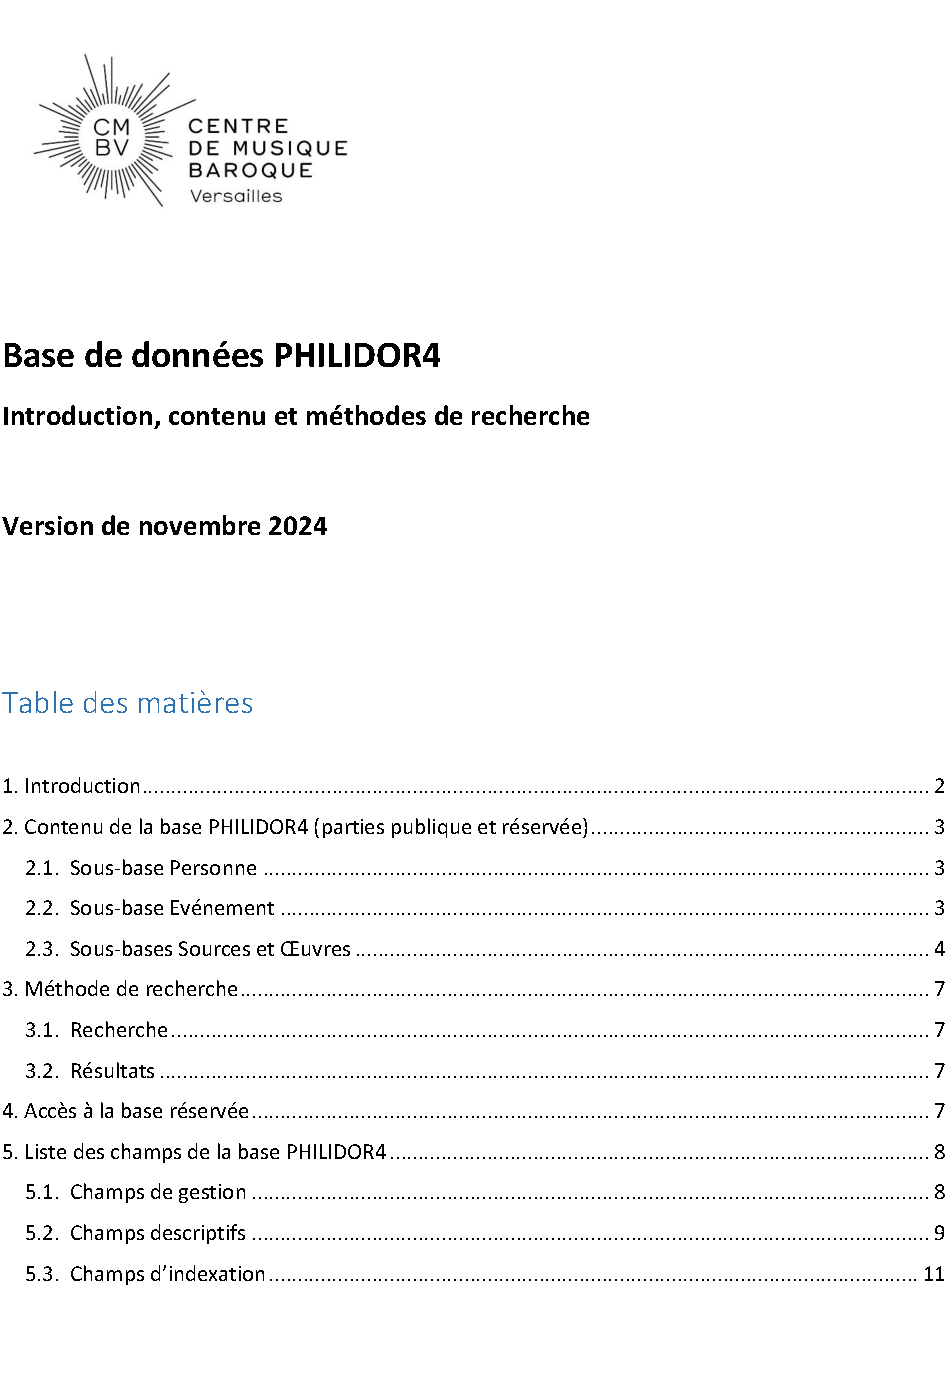
\includegraphics[page=1,width=0.7\textwidth,keepaspectratio]{pdf/PHILIDOR4 - Contenu et recherche cropped.pdf}
\end{center}

% Les pages suivantes, centrées aussi
\foreach \p in {2,...,11}{%
	\clearpage
	\begin{center}
		\includegraphics[page=\p,width=0.7\textwidth,keepaspectratio]{pdf/PHILIDOR4 - Contenu et recherche cropped.pdf}
	\end{center}
}
	
	\newpage{\pagestyle{empty}\cleardoublepage}
	
	%%%%%%%%%%%%%%%%%%
	
	\backmatter % glossaire, index, table des figures, table des matières.. (la bibliographie a déjà été appelée)
	
	%\printindex
	\printglossaries
	\listoftables
	\listoffigures
	\tableofcontents
\end{document}